\chapter{Adding New Methods}

\section{Code Directives}\label{sec:CodeDirectives}\index{directives}\index{code!directives}

\glc\ is designed to be flexible and extensible, allowing you to add new methods and functionality without having to hack the code extensively. To achieve this it makes much use of embedded code directives which, for example, explain to the build system how a particular subroutine or function connects into the \glc\ code. Such code directives are indicated by lines beginning with {\tt !\#}, and take the form of short blocks of XML. For example, a typical code directive might look like:
\begin{verbatim}
 !# <accretionDisksMethod>
 !#  <unitName>Accretion_Disks_Shakura_Sunyaev_Initialize</unitName>
 !# </accretionDisksMethod>
\end{verbatim}
This directive would typically appear just prior to a subroutine which initializes the Shakura-Sunyaev accretion disk module (it could appear anywhere throughout that module, but it makes sense to keep it close to the subroutine that it references). The {\tt accretionDisksMethod} tag explains to the \glc\ build system that this module contains an implementation of black hole accretion disks. The {\tt unitName} tag specifies the name of a program unit which (in this case) should be called to initialize this accretion disk implementation. The build system will then insert appropriate {\tt use} and {\tt call} statements into the \glc\ code such that this routine will be called if and when accretion disks are required by \glc.

\section{Components}\index{components}

This section describes the internal structure of node components, and how a component is implemented.

\subsection{Component Structure}\index{components!structure}

Each node in the merger tree consists of an arbitrary number of ``components''. A component may represent a dark matter halo, a galactic disk or a black hole. A component has the following structure:
\begin{verbatim}
 type component
   double precision, allocatable, dimension(:,:) :: properties
   double precision, allocatable, dimension(:)   :: data
   type(history),    allocatable, dimension(:)   :: histories
   type(component),  pointer                     :: nextComponentOfType
 end type component
\end{verbatim}
The {\tt nextComponentOfType} pointer allows components to be strung together in linked lists, useful if, for example, the component represents a black hole and the node in question contains many black holes. The {\tt properties} array is a list of properties that define the component (e.g. mass, radius etc.) and which will be evolved by \glc's ODE solver. In fact, this array will contain both the values of these properties and their time derivatives as needed by the solver. The {\tt data} array contains any internal data needed for this component. Typically, these are things which do not change with time (or, at least, their change is not described by an ODE). The {\tt histories} array contains a set of time series (which can, in fact, be records of the history of the galaxy, records of future behavior or anything else). These are frequently used for holding, for example, the rate of mass recycling from stellar populations at future times in a component.

\subsection{Implementing a New Component}\index{components!implementing}

Implementing a new component involves writing a module which handles initialization of the component, creation and destruction, specifies how the component should evolve, sets up interaction with other components and handles output of component properties. Frequently, the easiest way to make a new component is to copy a previously existing one and modify it as needed. Details of the various functions that a component module must perform are given below.

\subsubsection{Component Initialization}\index{components!initialization}

When \glc\ starts, it initializes all available components. To be included in this initialization call, a component must include a {\tt treeNodeCreateInitialize} directive. Minimally, the initialization routine must check whether it has been selected by comparing the {\tt comopnentOption} argument to its name and, if so, increment {\tt comopnentTypeCount}. Typically, components will want to keep a record of whether or not they were selected, the value of {\tt componentTypeCount} after incrementing (it is used to index the component later), determine how many properties/data/histories are required, set up pointers for property methods and grab any pipes that it wants to use. An example of an initialization subroutine (taken from the exponential disk component) is given below, with annotations (lines beginning with $\rightarrow$):
\begin{lstlisting}[escapechar=@,breaklines,prebreak=\&,postbreak=\&]
@$\rightarrow$ Give the directive to indicate that we have a component that we want to be initialized.@
  !# <treeNodeCreateInitialize>
@$\rightarrow$ Specify the name of the subroutine to call to initialize the component.@
  !#  <unitName>Tree_Node_Methods_Exponential_Disk_Initialize</unitName>
@$\rightarrow$ Declare that this component implementation is to be selected by the {\tt treeNodeMethodDisk} parameter, and that ``{\tt exponential}'' (i.e. this implementation) should be the default choice.@
  !#  <optionName default="exponential">treeNodeMethodDisk</optionName>
  !# </treeNodeCreateInitialize>
@$\rightarrow$ Subroutine begins: must have two arguments.@
  subroutine Tree_Node_Methods_Exponential_Disk_Initialize(componentOption,componentTypeCount)
    use ISO_Varying_String
    ...
    implicit none
    type(varying_string), intent(in)    :: componentOption
    integer,              intent(inout) :: componentTypeCount
    type(varying_string)                :: message

@$\rightarrow$ First check if the selected implementation (i.e. the value of the {\tt treeNodeMethodDisk} parameter, passed in as {\tt componentOption} matches the name for this component.@
    if (componentOption == 'exponential') then
@$\rightarrow$ It does, record that our method has been selected and proceed to do other initialization.@
       methodSelected=.true.

@$\rightarrow$ Incremant the component count (required) and store this value for later reference.@
       componentTypeCount=componentTypeCount+1
       componentIndex=componentTypeCount

@$\rightarrow$ Display a message saying that we've been selected (not required).@
       message='Exponential disk method selected [component index '
       message=message//componentIndex//']'
       call Galacticus_Display_Message(message,verbosityInfo)

@$\rightarrow$ Figure out how many properties and data we will need. In this case, we need to have enough to hold abundances and stellar luminosities in addition to some basic properties of the disk.@
       abundancesCount=Abundances_Property_Count()
       luminositiesCount=Stellar_Population_Luminosities_Count()
       propertyCount=propertyCountBase+2*abundancesCount+luminositiesCount
       dataCount    =dataCountBase

@$\rightarrow$ Now assign some indices for properties and data, so that we know where to find them in the component.@
       gasAbundancesIndex         =propertyCountBase                          +1
       gasAbundancesIndexEnd      =gasAbundancesIndex       +abundancesCount  -1
       stellarAbundancesIndex     =gasAbundancesIndexEnd                      +1
       stellarAbundancesIndexEnd  =stellarAbundancesIndex   +abundancesCount  -1
       stellarLuminositiesIndex   =stellarAbundancesIndexEnd                  +1
       stellarLuminositiesIndexEnd=stellarLuminositiesIndex +luminositiesCount-1

@$\rightarrow$ Associated procedure pointers for all properties, methods etc. In each case we must assign pointers to get and set values, adjust the rate of change for a property and to compute the rate of change. In some cases, these can be set to null or dummy values. (Not all properties shown beloe for brevity.)@
       Tree_Node_Disk_Radius                                  => Exponential_Disk_Radius
       Tree_Node_Disk_Radius_Set                              => null()
       Tree_Node_Disk_Radius_Rate_Adjust                      => null()
       Tree_Node_Disk_Radius_Rate_Compute                     => Tree_Node_Rate_Rate_Compute_Dummy

       Tree_Node_Disk_Gas_Mass                                => Tree_Node_Disk_Gas_Mass_Exponential
       Tree_Node_Disk_Gas_Mass_Set                            => Tree_Node_Disk_Gas_Mass_Set_Exponential
       Tree_Node_Disk_Gas_Mass_Rate_Adjust                    => Tree_Node_Disk_Gas_Mass_Rate_Adjust_Exponential
       Tree_Node_Disk_Gas_Mass_Rate_Compute                   => Tree_Node_Disk_Gas_Mass_Rate_Compute_Exponential

@$\rightarrow$  Grab pipes from other components. Here we want to grab the cooling pipe from the hot halo. Check it has not already been grabbed.@
       if (.not.associated(Tree_Node_Hot_Halo_Cooling_Mass_To)) then
          Tree_Node_Hot_Halo_Cooling_Mass_To => Tree_Node_Disk_Gas_Mass_Rate_Adjust_Exponential
       else
          call Galacticus_Error_Report('Tree_Node_Methods_Exponential_Disk_Initialize','expected to find unclaimed hot halo cooling pipe')
       end if

@$\rightarrow$ We're done initializing the component.@
    end if
    return
  end subroutine Tree_Node_Methods_Exponential_Disk_Initialize
\end{lstlisting}

\subsubsection{Component Creation and Destruction}\index{components!creation}\index{components!destruction}

When a node is created, it initially contains no components. A component must therefore create itself on the fly as needed. Typically, a component is first created when an attempt is made to set a property value, or to adjust the rate of change of a property value or in response to some event (e.g. a satellite component may be created in response to a node merging with a larger node). Requests for property values frequently \emph{do not} require that the component exist, as a zero value can often be returned instead. In such cases, it is useful to be able to check whether or not a component exists in a given node. This is done using {\tt thisNode\%componentExists(componentIndex)} where {\tt componentIndex} is the index stored during initialization.

Typically, we implement component creation within a function which returns the index of the current component within the {\tt components} array in the node. (This is not the same as {\tt componentIndex} and will vary from node to node depending on the order in which components were created for that node.) An example, taken from the exponential disk component, is given below, with annotations (lines beginning with $\rightarrow$):
\begin{lstlisting}[escapechar=@,breaklines,prebreak=\&,postbreak=\&]
@$\rightarrow$ Define a function that returns the index of the component in {\tt thisNode}.@
  integer function Tree_Node_Exponential_Disk_Index(thisNode)
    implicit none
    type(treeNode), pointer, intent(inout) :: thisNode
    integer                                :: thisIndex
    
@$\rightarrow$ Check if the component already exists\ldots@
    if (.not.thisNode%componentExists(componentIndex)) then
@$\rightarrow$ \ldots it does not, all {\tt createComponent} with the number of data, properties and histories required for this component.@
       call thisNode%createComponent(componentIndex,propertyCount,dataCount,historyCount)
@$\rightarrow$ Get the index within the {\tt components} array at which the component was created.@
       thisIndex=thisNode%componentIndex(componentIndex)
@$\rightarrow$ For this disk method, we call a routine to create the history component which will be used to store stellar properties.@
       call Stellar_Population_Properties_History_Create(thisNode,thisNode%components(thisIndex)%histories(stellarHistoryIndex))
    else
@$\rightarrow$ \ldots it does exist, simply get the index within the {\tt components} array at which the component is stored.@
       thisIndex=thisNode%componentIndex(componentIndex)
    end if
@$\rightarrow$ Return the result.@
    Tree_Node_Exponential_Disk_Index=thisIndex
    return
  end function Tree_Node_Exponential_Disk_Index
\end{lstlisting}
In this way, the rest of the module doesn't have to concern itself with creation---it simply requests the index of the component, knowing that it will be created as needed.

If necessary, a component can be destroyed using:
\begin{lstlisting}[escapechar=@,breaklines,prebreak=\&,postbreak=\&]
       call thisNode%destroyComponent(componentIndex,propertyCount,dataCount,historyCount)
\end{lstlisting}

\subsubsection{Component Methods}\index{components!methods}

Component methods provide a way for other components and functions within \glc\ to access the properties of a component, in a way that is independent of the specific component implementation chosen. To permit this, \glc\ will create a set of pointers which access methods for each property. For example, the exponential disk component has a ``stellar mass'' property. It informs \glc\ about this property using the directive:
\begin{lstlisting}[escapechar=@,breaklines,prebreak=\&,postbreak=\&]
  !# <treeNodeMethodsPointer>
  !#  <methodName>Tree_Node_Disk_Stellar_Mass</methodName>
  !# </treeNodeMethodsPointer>
\end{lstlisting}
This causes \glc\ to define four procedure pointers. The first two (the second two will be discussed below) are get and set methods for the property. The component, if selected, must associate these pointers which actual implementations during initialization. In our example case, this would require:
\begin{lstlisting}[escapechar=@,breaklines,prebreak=\&,postbreak=\&]
  Tree_Node_Disk_Stellar_Mass     => Tree_Node_Disk_Stellar_Mass_Exponential
  Tree_Node_Disk_Stellar_Mass_Set => Tree_Node_Disk_Stellar_Mass_Set_Exponential
\end{lstlisting}
The {\tt Tree\_Node\_Disk\_Stellar\_Mass\_Exponential} function must return the value of the stellar mass property and might look like:
\begin{lstlisting}[escapechar=@,breaklines,prebreak=\&,postbreak=\&]
  double precision function Tree_Node_Disk_Stellar_Mass_Exponential(thisNode)
    implicit none
    type(treeNode), pointer, intent(inout) :: thisNode
    integer                                :: thisIndex

    if (thisNode%componentExists(componentIndex)) then
       thisIndex=Tree_Node_Exponential_Disk_Index(thisNode)
       Tree_Node_Disk_Stellar_Mass_Exponential=thisNode%components(thisIndex)%properties(stellarMassIndex,propertyValue)
    else
       Tree_Node_Disk_Stellar_Mass_Exponential=0.0d0
    end if
    return
  end function Tree_Node_Disk_Stellar_Mass_Exponential
\end{lstlisting}
This function first checks whether or not an exponential disk component exists in this node. If it does, it finds the index of that node and then returns the value of the stellar mass property. If the component does not exist, it returns zero without causing a disk to be created.

The {\tt Tree\_Node\_Disk\_Stellar\_Mass\_Set\_Exponential} subroutine must set the stellar mass to the specified value, and might look like:
\begin{lstlisting}[escapechar=@,breaklines,prebreak=\&,postbreak=\&]
  subroutine Tree_Node_Disk_Stellar_Mass_Set_Exponential(thisNode,mass)
    implicit none
    type(treeNode),   pointer, intent(inout) :: thisNode
    double precision,          intent(in)    :: mass
    integer                                  :: thisIndex

    thisIndex=Tree_Node_Exponential_Disk_Index(thisNode)
    thisNode%components(thisIndex)%properties(stellarMassIndex,propertyValue)=mass
    return
  end subroutine Tree_Node_Disk_Stellar_Mass_Set_Exponential
\end{lstlisting}
Here, we first get the index of our component in the node (which will cause the component to be created if it does not already exist as discussed above) and then set the stellar mass to the input value, {\tt mass}.

Note that both of these procedures can be left {\tt null()}. Any attempt to call them will then cause the code to crash. Alternatively, an unsettable property could simply refuse to honor a request to set its value, either ignoring it, or exiting with an error message.

\subsubsection{Component Evolution}\index{evolution}\index{components!evolution}

All component properties are included in \glc's ODE solver as the node is evolved forward in time. \glc\ will create two pointers that permit the rate of change of a property to be computed and adjusted. These pointers should be associated with actual implementations during component initialization. For example, in the exponential disk component the stellar mass property pointers are set using:
\begin{lstlisting}[escapechar=@,breaklines,prebreak=\&,postbreak=\&]
   Tree_Node_Disk_Stellar_Mass_Rate_Adjust  => Tree_Node_Disk_Stellar_Mass_Rate_Adjust_Exponential
   Tree_Node_Disk_Stellar_Mass_Rate_Compute => Tree_Node_Disk_Stellar_Mass_Rate_Compute_Exponential
\end{lstlisting}

The ``rate adjust'' subroutine should look something like:
\begin{lstlisting}[escapechar=@,breaklines,prebreak=\&,postbreak=\&]
  subroutine Tree_Node_Disk_Stellar_Mass_Rate_Adjust_Exponential(thisNode,interrupt,interruptProcedure,rateAdjustment)
    implicit none
    type(treeNode),   pointer, intent(inout) :: thisNode
    logical,                   intent(inout) :: interrupt
    procedure(),      pointer, intent(inout) :: interruptProcedure
    double precision,          intent(in)    :: rateAdjustment
    integer                                  :: thisIndex
    
    if (.not.thisNode%componentExists(componentIndex)) then
       if (rateAdjustment /= 0.0d0) then
          interrupt=.true.
          interruptProcedure => Exponential_Disk_Create
       end if
       return
    end if
    thisIndex=Tree_Node_Exponential_Disk_Index(thisNode)
    thisNode%components(thisIndex)%properties(stellarMassIndex,propertyDerivative)&
         &=thisNode%components(thisIndex)%properties(stellarMassIndex,propertyDerivative)+rateAdjustment
    return
  end subroutine Tree_Node_Disk_Stellar_Mass_Rate_Adjust_Exponential
\end{lstlisting}
Here, we first check if an exponential disk component exists. If it does not, and the given {\tt rateAdjustment} is non-zero, then we need to create a disk component before we can adjust the rate. Since we are in the process of solving a set of ODEs which do not currently include the disk properties (since no disk exists) we need to interrupt the evolution and create a disk. This is done by setting {\tt interrupt-.true.} and setting {\tt interruptProcedure} to point to a procedure which will create a disk, and then returning. Interrupts will be discussed in more detail below. If the compoent does already exist, we simply find its index in the {\tt components} array and add {\tt rateAdjustment} to the current rate of change for the stellar mass property.

The ``rate compute'' subroutine should simply perform any calculations necessary to determine the rate of change of the property and adjust the rate appropriately\footnote{Actually, a single rate compute subroutine can compute and adjust rates for multiple properties within a component. Often this is convenient as their rates are related. In that case, the rate compute subroutines for those other properties can be left empty, or the relevant pointer let unset (it will be set to point to a dummy rate compute subroutine by default).}. Below is an example of the rate compute subroutine for the stellar mass property of the exponential disk component, with only the basic structure shown:
\begin{lstlisting}[escapechar=@,breaklines,prebreak=\&,postbreak=\&]
  subroutine Tree_Node_Disk_Stellar_Mass_Rate_Compute_Exponential(thisNode,interrupt,interruptProcedureReturn)
    implicit none
    type(treeNode),            pointer, intent(inout)       :: thisNode
    logical,                            intent(inout)       :: interrupt
    procedure(),               pointer, intent(inout)       :: interruptProcedureReturn
 
    if (thisNode%componentExists(componentIndex)) then
      ...
      call Tree_Node_Disk_Stellar_Mass_Rate_Adjust_Exponential(thisNode,interrupt,interruptProcedure,stellarMassRate)
      ...
    end if
    return
  end subroutine Tree_Node_Disk_Stellar_Mass_Rate_Compute_Exponential
\end{lstlisting}
Here, we simply check that the component exists and, if it does, compute the rates of change for one or more properties and then adjust their rates appropriately.

\subsubsection{Component Pipes}\index{pipes}\index{components!pipes}

Pipes can be thought of as interfaces between components that allow information to flow from one to the other. For example, suppose that a component representing the hot halo computes a rate of mass drop out due to cooling. This mass should flow into a galaxy component (typically the disk). To facilitate this, the hot halo component can define a pipe such as:
\begin{verbatim}
  !# <treeNodePipePointer>
  !#  <pipeName>Tree_Node_Hot_Halo_Cooling_To</pipeName>
  !# </treeNodePipePointer>
\end{verbatim}
Here {\tt Tree\_Node\_Hot\_Halo\_Cooling\_To} is a pointer to a {\tt rate-adjust} subroutine. During initialization, some other component can claim this pointer, and make it point to the {\tt rate-adjust} subroutine of one of their properties (e.g. the disk component could point it to the {\tt rate-adjust} subroutine for its gas mass property). Then, the hot halo component, after determining the rate of mass drop out, simply calls {\tt Tree\_Node\_Hot\_Halo\_Cooling\_To} with the appropriate node and rate to cause this mass to flow into the disk. 

This approach means that the hot halo component doesn't need to know in advance where the mass should be directed. This allows for the possibility that a different module is added to handle disks (for example), or that the cooling gas is to be directed to some other component.

Pipes are initialized to point to {\tt null()}. The defining component can choose to leave them this way, in which case it should either check that they have been associated before calling them and, if they haven't, either decide to not care or to exit gracefully with an error. Alternatively, the defining component can, on finding an unassociated pipe, point it to {\tt Tree\_Node\_Rate\_Adjust\_Dummy} which acts as a sink function---any rate adjustment passed into it is simply ignored. This is useful if, for example, we don't care where the mass cooling out of the hot halo goes in some instances.

\subsubsection{Evolution Interrupts}\index{interrupts}\index{evolution!interrupt}

It is often necessary to interrupt the smooth ODE evolution of a node in \glc. This can happen if, for example, a galaxy mergers with another galaxy (in which case the merger must be processed prior to further evolution) or if a component must be created before evolution can continue. The rate adjust and rate compute subroutines allow for interrupts to be flagged via their {\tt interrupt} and {\tt interruptProcedure} arguments. If an interrupt is required then {\tt interrupt} should be set to true, while {\tt interruptProcedure} should be set to point to a procedure which will handle the interrupt. Then, providing no other interrupt occurred earlier, the evolution will be stopped and the interrupt procedure called before evolution is continued.

An interrupt procedure should have the form:
\begin{lstlisting}[escapechar=@,breaklines,prebreak=\&,postbreak=\&]
  subroutine My_Interrupt_Procedure(thisNode)
    implicit none
    type(treeNode), pointer, intent(inout) :: thisNode
  
    ! Do whatever needs to be done to handle the interrupt.

    return
  end subroutine My_Interrupt_Procedure
\end{lstlisting}

\subsubsection{Sterile Methods}

A \emph{sterile} method is one which acts like a regular property but is not part of the {\tt properties()} array. For example, it may return a value from the {\tt data()} array, or some other function. Sterile methods can be created as a regular method, but with the {\tt set} and {\tt rate-adjust} subroutines left pointing to {\tt null()}. The {\tt rate-compute} method should be set to point to {\tt Tree\_Node\_Rate\_Rate\_Compute\_Dummy} which is a dummy {\tt rate-compute} procedure (i.e. it does nothing).

\section{Existing Method Types}

\subsection{Functions}

Functions implement basic calculations (e.g. computing the power spectrum).

\subsubsection{Accretion Disks}\label{sec:AccretionDisks}

Additional methods for accretion disk properties can be added using the {\tt accretionDisksMethod} directive. The directive should contain a single argument, giving the name of a subroutine to be called to initialize the method. For example, the {\tt Shakura-Sunyae} method is described by a directive:
\begin{verbatim}
 !# <accretionDisksMethod>
 !#  <unitName>Accretion_Disks_Shakura_Sunyaev_Initialize</unitName>
 !# </accretionDisksMethod>
\end{verbatim}
Here, {\tt Accretion\_Disks\_Shakura\_Sunyaev\_Initialize} is the name of a subroutine which will be called to initialize the method. The initialization subroutine must have the following form:
\begin{verbatim}
  subroutine Method_Initialize(accretionDisksMethod,Accretion_Disk_Radiative_Efficiency_Get,Black_Hole_Spin_Up_Rate_Get,Accretion_Disk_Jet_Power_Get)
    implicit none
    type(varying_string),          intent(in)    :: accretionDisksMethod
    procedure(),          pointer, intent(inout) :: Accretion_Disk_Radiative_Efficiency_Get,Black_Hole_Spin_Up_Rate_Get,Accretion_Disk_Jet_Power_Get
    
    if (accretionDisksMethod == 'myMethod') then
       Accretion_Disk_Radiative_Efficiency_Get => My_Accretion_Disk_Radiative_Efficiency_Get
       Black_Hole_Spin_Up_Rate_Get             => My_Black_Hole_Spin_Up_Rate_Get
       Accretion_Disk_Jet_Power_Get            => My_Accretion_Disk_Jet_Power_Get
    end if
    return
  end subroutine Method_Initialize
\end{verbatim}
where {\tt myMethod} is the name of this method as will be specified by the {\tt accretionDisksMethod} input parameter. The procedure pointers {\tt Accretion\_Disk\_Radiative\_Efficiency\_Get}, {\tt Black\_Hole\_Spin\_Up\_Rate\_Get} and {\tt Accretion\_Disk\_Jet\_Power\_Get} must be set to point to functions which return the radiative efficiency, black hole spin up rate and jet power for the accretion disk respectively as described below. The initialization subroutine should perform any other tasks required to initialize the module (such as reading parameters etc.).

The radiative efficiency function must have the form:
\begin{verbatim}
 double precision function My_Accretion_Disk_Radiative_Efficiency_Get(thisNode,massAccretionRate)
    implicit none
    type(treeNode),   intent(inout), pointer :: thisNode
    double precision, intent(in)             :: massAccretionRate
    .
    .
    .
    return
 end function My_Accretion_Disk_Radiative_Efficiency_Get
\end{verbatim}
The function must return the radiative efficiency for the accretion disk in {\tt thisNode}. The black hole spin function must have the form:
\begin{verbatim}
 double precision function My_Black_Hole_Spin_Up_Rate_Get(thisNode,massAccretionRate)
    implicit none
    type(treeNode),   intent(inout), pointer :: thisNode
    double precision, intent(in)             :: massAccretionRate
    .
    .
    .
    return
 end function My_Black_Hole_Spin_Up_Rate_Get
\end{verbatim}
The function must return the spin-up rate for the black hole in {\tt thisNode} given the {\tt massAccretionRate}. The jet power function must have the form:
\begin{verbatim}
 double precision function My_Accretion_Disk_Jet_Power_Get(thisNode,massAccretionRate)
    implicit none
    type(treeNode),   intent(inout), pointer :: thisNode
    double precision, intent(in)             :: massAccretionRate
    .
    .
    .
    return
 end function My_Accretion_Disk_Jet_Power_Get
\end{verbatim}
The function must return (in units of $M_\odot$ (km/s)$^2$ Gyr$^{-1}$) the jet power for the black hole/accretion disk system in {\tt thisNode} given the {\tt massAccretionRate}.

Currently defined accretion disk methods are:
\begin{description}
 \item [{\tt Shakura-Sunyaev}] Computes the properties of a thin, radiatively efficiency accretion disk.
 \item [{\tt ADAF}] Computes the properties of an ADAF using the model of \cite{benson_maximum_2009}.
 \item [{\tt switched}] Select either {\tt Shakura-Sunyaev} or {\tt ADAF} accretion disks based on the accretion rate:
 \begin{eqnarray}
  \dot{m}_{\rm minimum} < \dot{M}_{\bullet, 0}/\dot{M}_{\rm Eddington} < \dot{m}_{\rm maximum} &\rightarrow& \hbox{ Shakura-Sunyaev} \nonumber \\
  \hbox{otherwise } &\rightarrow& \hbox{ ADAG},
 \end{eqnarray}
 where $\dot{m}_{\rm minimum}$={\tt accretionRateThinDiskMinimum} and $\dot{m}_{\rm maximum}$={\tt accretionRateThinDiskMaximum} are input parameters.
\end{description}

\subsubsection{Accretion Onto Halos}

Additional methods for accretion of baryons onto halos can be added using the {\tt accretionHalosMethod} directive. The directive should contain a single argument, giving the name of a subroutine to be called to initialize the method. For example, the {\tt simple} method is described by a directive:
\begin{verbatim}
 !# <accretionHalosMethod>
 !#  <unitName>Accretion_Halos_Simple_Initialize</unitName>
 !# </accretionHalosMethod>
\end{verbatim}
Here, {\tt Accretion\_Halos\_Simple\_Initialize} is the name of a subroutine which will be called to initialize the method. The initialization subroutine must have the following form:
\begin{verbatim}
  subroutine Method_Initialize(accretionHalosMethod,Halo_Baryonic_Accretion_Rate_Get,Halo_Baryonic_Accreted_Mass_Get,Halo_Baryonic_Failed_Accretion_Rate_Get,Halo_Baryonic_Failed_Accreted_Mass_Get)
    implicit none
    type(varying_string),          intent(in)    :: accretionHalosMethod
    procedure(),          pointer, intent(inout) :: Halo_Baryonic_Accretion_Rate_Get,Halo_Baryonic_Accreted_Mass_Get,Halo_Baryonic_Failed_Accretion_Rate_Get,Halo_Baryonic_Failed_Accreted_Mass_Get
    
    if (accretionHalosMethod == 'myMethod') then
       Halo_Baryonic_Accretion_Rate_Get        => My_Accretion_Rate_Simple_Get
       Halo_Baryonic_Accreted_Mass_Get         => My_Accreted_Mass_Simple_Get
       Halo_Baryonic_Failed_Accretion_Rate_Get => My_Failed_Accretion_Rate_Simple_Get
       Halo_Baryonic_Failed_Accreted_Mass_Get  => My_Failed_Accreted_Mass_Simple_Get
    end if
    return
  end subroutine Method_Initialize
\end{verbatim}
where {\tt myMethod} is the name of this method as will be specified by the {\tt accretionHalosMethod} input parameter. The procedure pointers {\tt Halo\_Baryonic\_Accretion\_Rate\_Get}, {\tt Halo\_Baryonic\_Accreted\_Mass\_Get}, {\tt Halo\_Baryonic\_Failed\_Accretion\_Rate\_Get} and {\tt Halo\_Baryonic\_Failed\_Accreted\_Mass\_Get} must be set to point to functions which return accretion rate, total accreted mass (assuming no progenitors), failed accretion rate and total failed accreted mass (assuming no progenitors) respectively as described below. The initialization subroutine should perform any other tasks required to initialize the module (such as reading parameters etc.).

The functions must have the form:
\begin{verbatim}
 double precision function My_Accretion_Get(thisNode)
    implicit none
    type(treeNode),   intent(inout), pointer :: thisNode
    .
    .
    .
    return
 end function My_Accretion_Get
\end{verbatim}
In the case of the accretion rate functions, the function must return the accretion rate of baryons from the \IGM\ onto {\tt thisNode} in $M_\odot$ Gyr$^{-1}$. For total accreted mass functions, the total mass of baryons (in $M_\odot$) accreted onto {\tt thisNode} should be returned under the assumption that {\tt thisNode} formed instataneously with no progenitors. The ``failed'' accretion refers to mass which would have been accreted onto the halo if it simply traced the growth of overall mass. That is:
\begin{equation}
 \dot{M}_{\rm failed} = {\Omega_{\rm b} \over \Omega_0} \dot{M} - \dot{M}_{\rm accreted},
\end{equation}
where $\dot{M}$ is the growth rate of total halo mass and $\dot{M}_{\rm accreted}$ is the accretion rate of baryons onto the halo. If desired, this failed mass can be transferred back into the accreted component once the halo is deemed able to accrete, by simply adjusting the accretion rates returned appropriately.

Currently defined accretion disk methods are:
\begin{description}
 \item [{\tt simple}] Assumes that halos accrete all available baryons if they have virial velocities above {\tt reionizationSuppressionVelocity} or exist prior to redshift {\tt reionizationSuppressionRedshift}. This is a simple model of the effects of reionization on gas accretion. In halos which cannot accrete, accretion is placed into the failed mode. In halos which can accrete, any gas in the failed reservoir is returned to the accreted channel on a timescale of $\dot{M}/M$.
\end{description}

\subsubsection{Black Hole Binary Mergers}\label{sec:BlackHoleBinaryMergers}

Additional methods for black hole binary merger calculations can be added using the {\tt blackHoleBinaryMergersMethod} directive. The directive should contain a single argument, giving the name of a subroutine to be called to initialize the method. For example, the {\tt Rezzolla2008} method is described by a directive:
\begin{verbatim}
 !# <blackHoleBinaryMergersMethod>
 !#  <unitName>Black_Hole_Binary_Merger_Initialize</unitName>
 !# </blackHoleBinaryMergersMethod>
\end{verbatim}
Here, {\tt Black\_Hole\_Binary\_Merger\_Initialize} is the name of a subroutine which will be called to initialize the method. The initialization subroutine must have the following form:
\begin{verbatim}
  subroutine Method_Initialize(blackHoleBinaryMergersMethod,Black_Hole_Binary_Merger_Do)
    implicit none
    type(varying_string),          intent(in)    :: blackHoleBinaryMergersMethod
    procedure(),          pointer, intent(inout) :: Black_Hole_Binary_Merger_Do
    
    if (blackHoleBinaryMergersMethod == 'myMethod') Black_Hole_Binary_Merger_Do => My_Method_Do_Procedure
    return
  end subroutine Method_Initialize
\end{verbatim}
where {\tt myMethod} is the name of this method as will be specified by the {\tt blackHoleBinaryMergersMethod} input parameter. The procedure pointer {\tt Black\_Hole\_Binary\_Merger\_Do} must be set to point to a function which returns the properties (mass and spin) of the merged black hole as described below. The initialization subroutine should perform any other tasks required to initialize the module (such as reading parameters etc.).

The cooling radius function must have the form:
\begin{verbatim}
 subroutine My_Method_Do_Procedure(blackHoleMassA,blackHoleMassB,blackHoleSpinA,blackHoleSpinB,blackHoleMassFinal,blackHoleSpinFinal)
    implicit none
    double precision, intent(in)  :: blackHoleMassA,blackHoleMassB,blackHoleSpinA,blackHoleSpinB
    double precision, intent(out) :: blackHoleMassFinal,blackHoleSpinFinal
    .
    .
    .
    return
 end subroutine My_Method_Do_Procedure
\end{verbatim}
The function must return the mass and spin (in {\tt blackHoleMassFinal} and {\tt blackHoleSpinFinal} respectively) of the black hole resulting from the merger of black holes with masses {\tt blackHoleMassA} and {\tt blackHoleMassB} and spins {\tt blackHoleSpinA} and {\tt blackHoleSpinB}. The subroutine should make no assumptions about the mass ordering of the input black holes (i.e. A could be more massive than B or vice versa).

Currently defined black hole binary merger methods are:
\begin{description}
 \item [{\tt Rezzolla2008}] Computes the properties of the merged black hole using the approximations of \cite{rezzolla_final_2008}.
\end{description}

\subsubsection{Cooling Rate}

Additional methods for the cooling rate from the hot halo can be added using the {\tt coolingRateMethod} directive. The directive should contain a single argument, giving the name of a subroutine to be called to initialize the method. For example, the {\tt White + Frenk} method is described by a directive:
\begin{verbatim}
 !# <coolingRateMethod>
 !#  <unitName>Cooling_Rate_White_Frenk_Initialize</unitName>
 !# </coolingRateMethod>
\end{verbatim}
Here, {\tt Cooling\_Rate\_White\_Frenk\_Initialize} is the name of a subroutine which will be called to initialize the method. The initialization subroutine must have the following form:
\begin{verbatim}
  subroutine Method_Initialize(coolingRateMethod,Cooling_Rate_Get)
    implicit none
    type(varying_string),          intent(in)    :: coolingRateMethod
    procedure(),          pointer, intent(inout) :: Cooling_Rate_Get
    
    if (coolingRateMethod == 'myMethod') Cooling_Rate_Get => My_Method_Get
    return
  end subroutine Method_Initialize
\end{verbatim}
where {\tt myMethod} is the name of this method as will be specified by the {\tt coolingRateMethod} input parameter. The procedure pointer {\tt Cooling\_Rate\_Get} must be set to point to a function which returns the cooling rate from the hot halo. The initialization subroutine should perform any other tasks required to initialize the module (such as reading parameters etc.).

The cooling rate function must have the form:
\begin{verbatim}
 double precision function Cooling_Rate_Get(thisNode)
    implicit none
    type(treeNode),   intent(inout), pointer :: thisNode
    .
    .
    .
    return
 end function Cooling_Rate_Get
\end{verbatim}
The function must return the rate of mass drop-out from the hot halo (in units of $M_\odot$/Gyr) for {\tt thisNode}. 

Currently defined cooling rate methods are:
\begin{description}
 \item [\hyperlink{cooling.cooling_rate.White-Frenk.F90:cooling_rates_white_frenk:cooling_rate_white_frenk}{{\tt White + Frenk}}] Implements something similar to that proposed by \cite{white_galaxy_1991}. Namely, the cooling rate is set equal to
 \begin{equation}
  \dot{M}_{\rm cool} = 4 \pi \rho(r_{\rm cool}) r_{\rm cool}^2 \dot{r}_{\rm cool}
 \end{equation}
 if the cooling radius is within the virial radius and
 \begin{equation}
  \dot{M}_{\rm cool} = {M_{\rm hot} \over \tau_{\rm dynamical,halo}}
 \end{equation}
 otherwise.
\end{description}

\subsubsection{Cooling Function}\label{sec:CoolingFunctionMethods}

Additional methods for cooling functions can be added using the {\tt coolingFunctionMethods}, {\tt coolingFunctionCompute}, {\tt coolingFunctionDensitySlopeCompute} and {\tt coolingFunctionTemperatureSlopeCompute} directives. Each directive should contain a single argument, giving the name of a subroutine to be called to either initialize the method or compute the relevant quantity. For example, the {\tt atomic CIE Cloudy} method is initialized by a directive:
\begin{verbatim}
  !# <coolingFunctionMethods>
  !#  <unitName>Cooling_Function_Atomic_CIE_Cloudy_Initialize</unitName>
  !# </coolingFunctionMethods>
\end{verbatim}
Here, {\tt Cooling\_Function\_Atomic\_CIE\_Cloudy\_Initialize} is the name of a subroutine which will be called to initialize the method. The initialization subroutine must have the following form:
\begin{verbatim}
  subroutine Method_Initialize(coolingFunctionMethods)
    implicit none
    type(varying_string), intent(in) :: coolingFunctionMethods(:)
    
    if (any(coolingFunctionMethods == 'myMethod')) then
       .
       .
       .
    end if
    return
  end subroutine Method_Initialize
\end{verbatim}
where {\tt myMethod} is the name of this method as will be specified by the {\tt coolingFunctionMethods} input parameter. The initialization routine should record that whether this cooling function was selected, and perform any other initialization necessary.

The other directives should specify subroutines with the following template:
\begin{verbatim}
  subroutine Cooling_Function_PropertyCompute(coolingFunctionProperty,temperature,numberDensityHydrogen,abundances&
       &,radiation)
    implicit none
    double precision,          intent(in)  :: temperature,numberDensityHydrogen
    type(abundancesStructure), intent(in)  :: abundances
    type(radiationStructure),  intent(in)  :: radiation
    double precision,          intent(out) :: coolingFunctionProperty
    .
    .
    .
    return
  end subroutine Cooling_Function_PropertyCompute
\end{verbatim}
and each should return the relevant quantity in {\tt coolingFunctionProperty}. The {\tt coolingFunctionCompute} subroutine should return the cooling function, the {\tt coolingFunctionDensitySlopeCompute} subroutine should return the partial derivative with respect to hydrogen density and the {\tt coolingFunctionTemperatureSlopeCompute} subroutine should return the partial derivative with respect to temperature.

Currently defined cooling function methods are:
\begin{description}
 \item [\hyperlink{cooling.cooling_function.CIE_file.F90:cooling_functions_cie_file:cooling_function_cie_file}{{\tt CIE\_from\_file}}] Reads a tabulated CIE cooling function from a file and interpolates in the table to give a result. The XML file containing the table should have the following form:
 \begin{verbatim}
  <coolingFunctions>
  <coolingFunction>
    <temperature>
      <datum>10000.0</datum>
      <datum>15000.0</datum>
      .
      .
      .
    </temperature>
    <coolingRate>
      <datum>1.0e-23</datum>
      <datum>1.7e-23</datum>
      .
      .
      .
    </coolingRate>
    <metallicity>-4.0</metallicity>
  </coolingFunction>
  <coolingFunction>
  .
  .
  .
  </coolingFunction>
  <description>Some description of what this cooling function is.</description>
  <extrapolation>
    <metallicity>
      <limit>low</limit>
      <method>power law</method>
    </metallicity>
    <metallicity>
      <limit>high</limit>
      <method>power law</method>
    </metallicity>
    <temperature>
      <limit>low</limit>
      <method>power law</method>
    </temperature>
    <temperature>
      <limit>high</limit>
      <method>power law</method>
    </temperature>
  </extrapolation>
 </coolingFunctions>
 \end{verbatim}
 Each {\tt coolingFunction} element should contain two lists (inside {\tt temperature} and {\tt coolingRate} tags) of {\tt datum} elements which specify temperature (in Kelvin) and cooling function (in ergs cm$^3$ s$^{-1}$ computed for a hydrogen density of 1 cm$^{-3}$) respectively, and a {\tt metallicity} element which gives the logarithmic metallcity relative to Solar (a value of -999 or less is taken to imply zero metallicity). Any number of {\tt coolingFunction} elements may appear, but they must be in order of increasing metallicity and must all contain the same set of temperatures. The {\tt extrapolation} element defines how the table is to be extrapolated in the {\tt low} and {\tt high} limits of {\tt temperature} and {\tt metallicity}. The {\tt method} elements can take the following values:
 \begin{description}
  \item[{\tt zero}] The cooling function is set to zero beyond the relevant limit.
  \item[{\tt fixed}] The cooling function is held fixed at the value at the relevant limit.
  \item[{\tt power law}] The cooling function is extrapolated assuming a power-law dependence beyond the relevant limit. This option is only allowed if the cooling function is everywhere positive.
 \end{description}
 If the cooling function is everywhere positive the interpolation will be done in the logarithmic of temperature, metallicity\footnote{The exception is if the first cooling function is tabulated for zero metallicity. In that case, a linear interpolation in metallicity is always used between zero and the first non-zero tabulated metallicity.} and cooling function. Otherwise, interpolation is linear in these quantities. The cooling function is scaled assuming a quadratic dependence on hydrogen density.
 \item [{\tt atomic\_CIE\_Cloudy}] Uses the {\sc Cloudy} software to compute a cooling function for atomic gas in collisional ionization equilibrium. {\sc Cloudy} will be downloaded, compiled and run automatically if necessary\footnote{{\sc Cloudy} is used to generate a file which contains a tabulation of the cooling function suitable for reading by the {\tt CIE from file} method. Generation of the tabulation typically takes several hours, but only needs to be done once as the stored table is simply read back in on later runs.}. Figure~\ref{fig:atomicCIECloudyCoolingFunction} shows the cooling function from this method.
 \item [{\tt CMB\_Compton}] Computes the cooling function due to Compton scattering off of \CMB\ photons.
\end{description}

\begin{figure}
 \begin{center}
 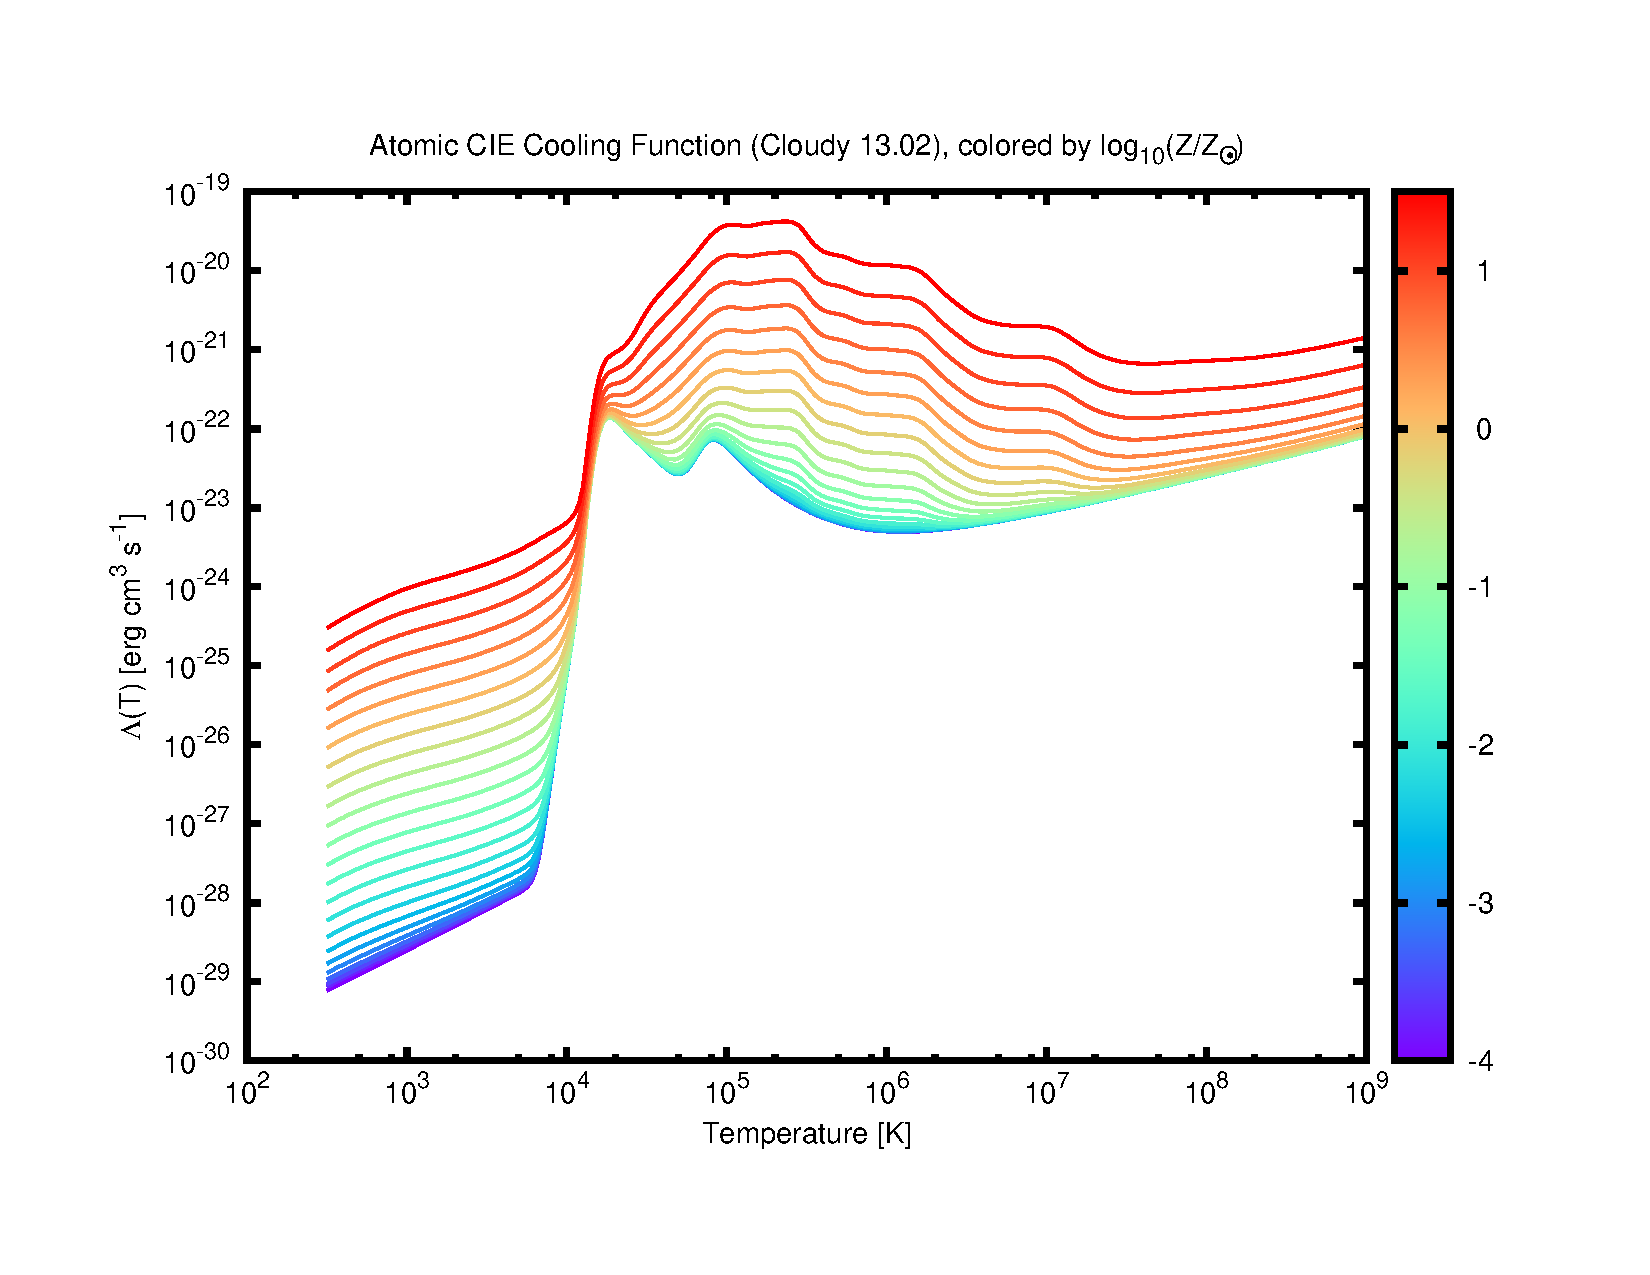
\includegraphics[width=160mm]{../plots/cooling_function_Atomic_CIE_Cloudy.pdf}
 \end{center}
 \caption{Cooling function for atomic gas in collisional ionization equilibrium computed using Cloudy 08.00.}
 \label{fig:atomicCIECloudyCoolingFunction}
\end{figure}

\subsubsection{Cooling Radius}

Additional methods for cooling radius calculations can be added using the {\tt coolingRadiusMethod} directive. The directive should contain a single argument, giving the name of a subroutine to be called to initialize the method. For example, the {\tt simple} method is described by a directive:
\begin{verbatim}
 !# <coolingRadiusMethod>
 !#  <unitName>Cooling_Radius_Simple_Initialize</unitName>
 !# </coolingRadiusMethod>
\end{verbatim}
Here, {\tt Cooling\_Radius\_Simple\_Initialize} is the name of a subroutine which will be called to initialize the method. The initialization subroutine must have the following form:
\begin{verbatim}
  subroutine Method_Initialize(coolingRadiusMethod,Cooling_Radius_Get,Cooling_Radius_Growth_Rate_Get)
    implicit none
    type(varying_string),          intent(in)    :: coolingRadiusMethod
    procedure(),          pointer, intent(inout) :: Cooling_Radius_Get,Cooling_Radius_Growth_Rate_Get
    
    if (coolingRadiusMethod == 'myMethod') then
       Cooling_Radius_Get => My_Method_Get_Procedure
       Cooling_Radius_Growth_Rate_Get => My_Method_Growth_Rate_Get_Procedure
    end if
    return
  end subroutine Method_Initialize
\end{verbatim}
where {\tt myMethod} is the name of this method as will be specified by the {\tt coolingRadiusMethod} input parameter. The procedure pointer {\tt Cooling\_Radius\_Get} must be set to point to a function which returns the cooling function as described below while {\tt Cooling\_Radius\_Growth\_Rate\_Get} should be set to point to a function which returns the rate at which the cooling radius is growing. The initialization subroutine should perform any other tasks required to initialize the module (such as reading parameters etc.).

The cooling radius function must have the form:
\begin{verbatim}
 double precision function Cooling_Radius_Get(thisNode)
    implicit none
    type(treeNode), intent(inout), pointer :: thisNode
    .
    .
    .
    return
 end function Cooling_Radius_Get
\end{verbatim}
The function must return the cooling radius (in units of Mpc) for {\tt thisNode}. The cooling radius growth rate function should have the same template but return the rate at which the cooling radius grows in units of Mpc/Gyr.

Currently defined cooling radius methods are:
\begin{description}
 \item [\hyperlink{cooling.cooling_radius.simple.F90:cooling_radii_simple:cooling_radius_simple}{{\tt simple}}] Computes the cooling radius by seeking the radius at which the time available for cooling equals the cooling time. The growth rate is determined consistently based on the slope of the density profile, the density dependence of the cooling function and the rate at which the time available for cooling is increasing. This method assumes that the cooling time is a monotonic function of radius.
\end{description}

\subsubsection{Cooling Rate}

Additional methods for the cooling rate from the hot halo can be added using the {\tt coolingRateMethod} directive. The directive should contain a single argument, giving the name of a subroutine to be called to initialize the method. For example, the {\tt White + Frenk} method is described by a directive:
\begin{verbatim}
 !# <coolingRateMethod>
 !#  <unitName>Cooling_Rate_White_Frenk_Initialize</unitName>
 !# </coolingRateMethod>
\end{verbatim}
Here, {\tt Cooling\_Rate\_White\_Frenk\_Initialize} is the name of a subroutine which will be called to initialize the method. The initialization subroutine must have the following form:
\begin{verbatim}
  subroutine Method_Initialize(coolingRateMethod,Cooling_Rate_Get)
    implicit none
    type(varying_string),          intent(in)    :: coolingRateMethod
    procedure(),          pointer, intent(inout) :: Cooling_Rate_Get
    
    if (coolingRateMethod == 'myMethod') Cooling_Rate_Get => My_Method_Get
    return
  end subroutine Method_Initialize
\end{verbatim}
where {\tt myMethod} is the name of this method as will be specified by the {\tt coolingRateMethod} input parameter. The procedure pointer {\tt Cooling\_Rate\_Get} must be set to point to a function which returns the cooling rate from the hot halo. The initialization subroutine should perform any other tasks required to initialize the module (such as reading parameters etc.).

The cooling rate function must have the form:
\begin{verbatim}
 double precision function Cooling_Rate_Get(thisNode)
    implicit none
    type(treeNode),   intent(inout), pointer :: thisNode
    .
    .
    .
    return
 end function Cooling_Rate_Get
\end{verbatim}
The function must return the rate of mass drop-out from the hot halo (in units of $M_\odot$/Gyr) for {\tt thisNode}. 

Currently defined cooling rate methods are:
\begin{description}
 \item [\hyperlink{cooling.cooling_rate.White-Frenk.F90:cooling_rates_white_frenk:cooling_rate_white_frenk}{{\tt White + Frenk}}] Implements something similar to that proposed by \cite{white_galaxy_1991}. Namely, the cooling rate is set equal to
 \begin{equation}
  \dot{M}_{\rm cool} = 4 \pi \rho(r_{\rm cool}) r_{\rm cool}^2 \dot{r}_{\rm cool}
 \end{equation}
 if the cooling radius is within the virial radius and
 \begin{equation}
  \dot{M}_{\rm cool} = {M_{\rm hot} \over \tau_{\rm dynamical,halo}}
 \end{equation}
 otherwise.
\end{description}

\subsubsection{Cooling Time}

Additional methods for cooling time calculations can be added using the {\tt coolingTimeMethod} directive. The directive should contain a single argument, giving the name of a subroutine to be called to initialize the method. For example, the {\tt simple} method is described by a directive:
\begin{verbatim}
 !# <coolingTimeMethod>
 !#  <unitName>Cooling_Time_Simple_Initialize</unitName>
 !# </coolingTimeMethod>
\end{verbatim}
Here, {\tt Cooling\_Time\_Simple\_Initialize} is the name of a subroutine which will be called to initialize the method. The initialization subroutine must have the following form:
\begin{verbatim}
  subroutine Method_Initialize(coolingTimeMethod,Cooling_Time_Get,Cooling_Time_Density_Log_Slope_Get,Cooling_Time_Temperature_Log_Slope_Get)
    implicit none
    type(varying_string),          intent(in)    :: coolingTimeMethod
    procedure(),          pointer, intent(inout) :: Cooling_Time_Get,Cooling_Time_Density_Log_Slope_Get,Cooling_Time_Temperature_Log_Slope_Get
    
    if (coolingTimeMethod == 'myMethod') then
       Cooling_Time_Get => My_Method_Get_Procedure
       Cooling_Time_Density_Log_Slope_Get => My_Method_Density_Log_Slope_Procedure
       Cooling_Time_Temperature_Log_Slope_Get => My_Method_Temperature_Log_Slope_Procedure
    end if
    return
  end subroutine Method_Initialize
\end{verbatim}
where {\tt myMethod} is the name of this method as will be specified by the {\tt coolingTimeMethod} input parameter. The procedure pointer {\tt Cooling\_Time\_Get} must be set to point to a function which returns the cooling function as described below while the other two pointers should point to functions which return the appropriate logarithmic slope. The initialization subroutine should perform any other tasks required to initialize the module (such as reading parameters etc.).

The cooling radius function must have the form:
\begin{verbatim}
 double precision function Cooling_Time_Get(temperature,density,abundances,radiation)
    implicit none
    double precision,          intent(in) :: temperature,density
    type(abundancesStructure), intent(in) :: abundances
    type(radiationStructure),  intent(in) :: radiation
    .
    .
    .
    return
 end function Cooling_Time_Get
\end{verbatim}
The function must return the cooling time (in units of Gyr) for at the specified {\tt temperature}, {\tt density} and for composition and radiation field as specified by the {\tt abundances} and {\tt radiation} structures. The logarithmic slope functions should have the same template, but return the logarithmic slope of the cooling time with respect to the appropriate variable instead.

Currently defined cooling time methods are:
\begin{description}
 \item [\hyperlink{cooling.cooling_time.simple.F90:cooling_times_simple:cooling_time_simple}{{\tt simple}}] Compute the cooling time as the ratio of the gas thermal energy density to the volume rate of radiative energy loss. The gas is assumed to have an effective number of degrees of freedom specified by the {\tt coolingTimeSimpleDegreesOfFreedom} parameter.
\end{description}

\subsubsection{Cosmology}\label{sec:CosmologyMethods}

Additional methods for cosmology can be added using the {\tt cosmologyMethod} directive. The directive should contain a single argument, giving the name of a subroutine to be called to initialize the method. For example, the {\tt matter + lambda} method is described by a directive:
\begin{verbatim}
  !# <cosmologyMethod>
  !#  <unitName>Cosmology_Functions_Matter_Lambda_Initialize</unitName>
  !# </cosmologyMethod>
\end{verbatim}
Here, {\tt Cosmology\_Functions\_Matter\_Lambda\_Initialize} is the name of a subroutine which will be called to initialize the method. The initialization subroutine must have the following form:
\begin{verbatim}
  subroutine Method_Initialize(cosmologyMethod,Expansion_Factor_Is_Valid_Get,Cosmic_Time_Is_Valid_Get &
       &,Cosmology_Age_Get,Expansion_Factor_Get,Hubble_Parameter_Get,Early_Time_Density_Scaling_Get  & 
       &,Omega_Matter_Get,Omega_Dark_Energy_Get,Expansion_Rate_Get,Epoch_of_Matter_Dark_Energy_Equality_Get &
       &,Epoch_of_Matter_Domination_Get,Epoch_of_Matter_Curvature_Equality_Get,CMB_Temperature_Get)
    implicit none
    type(varying_string),          intent(in)    :: cosmologyMethod
    procedure(),          pointer, intent(inout) :: Expansion_Factor_Is_Valid_Get,Cosmic_Time_Is_Valid_Get &
       &,Cosmology_Age_Get,Expansion_Factor_Get,Hubble_Parameter_Get,Early_Time_Density_Scaling_Get  & 
       &,Omega_Matter_Get,Omega_Dark_Energy_Get,Expansion_Rate_Get,Epoch_of_Matter_Dark_Energy_Equality_Get &
       &,Epoch_of_Matter_Domination_Get,Epoch_of_Matter_Curvature_Equality_Get,CMB_Temperature_Get
    
    if (cosmologyMethod == 'myMethod') then
       Procedure_Pointer_Get => My_Procedure
       .
       .
       .
    end if
    return
  end subroutine Method_Initialize
\end{verbatim}
where {\tt myMethod} is the name of this method as will be specified by the {\tt cosmologyMethod} input parameter. Numerous procedure pointers are passed in and should be set to point to functions/subroutines that perform cosmological calcalculations as described below. The initialization subroutine should perform any other tasks required to initialize the module (such as reading parameters etc.).

Below are a list of procedure templates for the various procedures required by the cosmology method. After each template a description of what the procedure must do is given.

\begin{verbatim}
   logical function My_Expansion_Factor_Is_Valid(aExpansion)
     implicit none
     double precision, intent(in) :: aExpansion
     .
     .
     .
     return
   end function My_Expansion_Factor_Is_Valid
\end{verbatim}
Should return true if the input expansion factor is valid (e.g. greater than zero and less the the maximum expansion factor for a collapsing universe).

\begin{verbatim}
   logical function My_Cosmic_Time_Is_Valid(time)
     implicit none
     double precision, intent(in) :: time
     .
     .
     .
     return
   end function My_Cosmic_Time_Is_Valid
\end{verbatim}
Should return true if the input cosmic time is valid (e.g. greater than zero and less than the time at the Big Crunch in collapsing universes).

\begin{verbatim}
   double precision function My_Cosmology_Age(aExpansion,collapsingPhase)
     implicit none
     double precision, intent(in)           :: aExpansion
     logical,          intent(in), optional :: collapsingPhase
     .
     .
     .
     return
   end function My_Cosmology_Age
\end{verbatim}
Should return the age (in Gyr) of the universe at a given expansion factor. The {\tt collapsingPhase} argument optionally specififies whether the age during the expanding or collapsing phase is required---if absent then the expanding phase should be assumed.

\begin{verbatim}
   double precision function My_Expansion_Factor(tCosmological)
     implicit none
     double precision, intent(in) :: tCosmological
     .
     .
     .
     return
   end function My_Expansion_Factor
\end{verbatim}
Should return the expansion factor of the universe at the input cosmological time (given in Gyr).

\begin{verbatim}
   double precision function My_Expansion_Rate(aExpansion)
     implicit none
     double precision, intent(in) :: aExpansion
     .
     .
     .
     return
   end function My_Expansion_Rate
\end{verbatim}
Should return the expansion rate, $\dot{a}/a$ (in Gyr$^{-1}$), at the given expansion factor.

\begin{verbatim}
   double precision function My_Hubble_Parameter(tCosmological,aExpansion,collapsingPhase)
     implicit none
     double precision, intent(in), optional :: tCosmological,aExpansion
     logical,          intent(in), optional :: collapsingPhase
     .
     .
     .
     return
   end function My_Hubble_Parameter
\end{verbatim}
Should return the Hubble parameter (in km/s/Mpc) at the given cosmic epoch. The cosmic epoch can be specified as a time since the Big Bang, or an expansion factor (in the expanding phase unless the collapsing phase is specifically requested). Specifying a time and an expansion factor is invalid input, and the routine should abort in such cases.

\begin{verbatim}
   subroutine My_Early_Time_Density_Scaling(dominateFactor,densityPower,aDominant,Omega_Dominant)
     implicit none
     double precision, intent(in)            :: dominateFactor
     double precision, intent(out)           :: densityPower,aDominant
     double precision, intent(out), optional :: Omega_Dominant
     .
     .
     .
     return
   end subroutine My_Early_Time_Density_Scaling
\end{verbatim}
Should compute the epoch, {\tt aDominant}, before which the universe is dominated by a single component (e.g. in a matter and cosmological constant only universe, the epoch before which matter always dominated). The epoch should be such that the component in question dominates over others in density by a factor of {\tt dominateFactor}. The exponent in the density-expansion factor relation for this relation should be returned in {\tt densityPower}. If present, {\tt Omega\_Dominant} should be set to the density of the dominant component (in units of the critical density) at the present day.

\begin{verbatim}
   double precision function My_Epoch_of_Matter_Domination(dominateFactor)
     implicit none
     double precision, intent(in) :: dominateFactor
      .
     .
     .
    return
   end function My_Epoch_of_Matter_Domination
\end{verbatim}
Should return the epoch at which matte dominates the energy density of the universe by the specified factor.

\begin{verbatim}
   double precision function My_Omega_Matter(tCosmological,aExpansion,collapsingPhase)
     implicit none
     double precision, intent(in), optional :: tCosmological,aExpansion
     logical,          intent(in), optional :: collapsingPhase
     .
     .
     .
     return
   end function My_Omega_Matter
\end{verbatim}
Should return $\Omega_{\rm M}$ at the given cosmic epoch. The cosmic epoch can be specified as a time since the Big Bang, or an expansion factor (in the expanding phase unless the collapsing phase is specifically requested). Specifying a time and an expansion factor is invalid input, and the routine should abort in such cases.

\begin{verbatim}
   double precision function My_Omega_Dark_Energy(tCosmological,aExpansion,collapsingPhase)
     implicit none
     double precision, intent(in), optional :: tCosmological,aExpansion
     logical,          intent(in), optional :: collapsingPhase
     .
     .
     .
     return
   end function My_Omega_Dark_Energy
\end{verbatim}
Should return $\Omega_\Lambda$ at the given cosmic epoch. The cosmic epoch can be specified as a time since the Big Bang, or an expansion factor (in the expanding phase unless the collapsing phase is specifically requested). Specifying a time and an expansion factor is invalid input, and the routine should abort in such cases.

\begin{verbatim}
   double precision function My_Epoch_of_Matter_Dark_Energy_Equality(requestType)
     implicit none
     integer, intent(in) :: requestType
     .
     .
     .
     return
   end function My_Epoch_of_Matter_Dark_Energy_Equality
\end{verbatim}
Should return the cosmic epoch at which matter and dark energy have equal energy densities. If {\tt requestType} is {\tt requestTypeTime} (specified in the {\tt Cosmology\_Functions\_Parameters} module) then cosmic time (in Gyr) should be returned, while if it is {\tt requestTypeExpansionFactor} then expansion factor should be returned instead.

\begin{verbatim}
   double precision function My_Epoch_of_Matter_Curvature_Equality(requestType)
     implicit none
     integer, intent(in) :: requestType
     .
     .
     .
     return
   end function My_Epoch_of_Matter_Curvature_Equality
\end{verbatim}
Should return the cosmic epoch at which matter and curvature have equal energy densities. If {\tt requestType} is {\tt requestTypeTime} (specified in the {\tt Cosmology\_Functions\_Parameters} module) then cosmic time (in Gyr) should be returned, while if it is {\tt requestTypeExpansionFactor} then expansion factor should be returned instead.

\begin{verbatim}
   double precision function My_CMB_Temperature(tCosmological,aExpansion,collapsingPhase)
     implicit none
     double precision, intent(in), optional :: tCosmological,aExpansion
     logical,          intent(in), optional :: collapsingPhase
     .
     .
     .
     return
   end function My_CMB_Temperature
\end{verbatim}
Should return the \CMB\ temperature (in K) at the given cosmic epoch. The cosmic epoch can be specified as a time since the Big Bang, or an expansion factor (in the expanding phase unless the collapsing phase is specifically requested). Specifying a time and an expansion factor is invalid input, and the routine should abort in such cases.

Currently defined cosmology methods are:
\begin{description}
 \item [{\tt matter + lambda}] Cosmological relations are computed assuming a universe that contains only matter and a cosmological constant.
\end{description}

\subsubsection{Critical Overdensity for Halo Collapse}

Additional methods for the critical linear theory overdensity for halo collapse can be added using the {\tt criticalOverdensityMethod} directive. The directive should contain a single argument, giving the name of a subroutine to be called to initialize the method. For example, the {\tt spherical top hat} method is described by a directive:
\begin{verbatim}
  !# <criticalOverdensityMethod>
  !#  <unitName>Spherical_Collape_Delta_Critical_Initialize</unitName>
  !# </criticalOverdensityMethod>
\end{verbatim}
Here, {\tt Spherical\_Collape\_Delta\_Critical\_Initialize} is the name of a subroutine which will be called to initialize the method. The initialization subroutine must have the following form:
\begin{verbatim}
  subroutine Method_Initialize(criticalOverdensityMethod,Critical_Overdensity_Tabulate)
    implicit none
    type(varying_string),          intent(in)    :: criticalOverdensityMethod
    procedure(),          pointer, intent(inout) :: Critical_Overdensity_Tabulate
    
    if (criticalOverdensityMethod.eq.'myMethod') then
       Critical_Overdensity_Tabulate => My_Do_Tabulate
       .
       .
       .
    end if
    return
  end subroutine Method_Initialize
\end{verbatim}
where {\tt myMethod} is the name of this method as will be specified by the {\tt criticalOverdensityMethod} input parameter. The procedure pointer {\tt Critical\_Overdensity\_Tabulate} must be set to point to a subroutine which tabulates the critical overdensity as described below. The initialization subroutine should perform any other tasks required to initialize the module (such as reading parameters etc.).

The tabulation subroutine must have the form:
\begin{verbatim}
   subroutine Critical_Overdensity_Tabulate(time,deltaCritNumberPoints,deltaCritTime,deltaCritDeltaCrit)
    implicit none
    double precision, intent(in)                               :: time
    integer,          intent(out)                              :: deltaCritNumberPoints
    double precision, intent(inout), allocatable, dimension(:) :: deltaCritTime,deltaCritDeltaVirial
    .
    .
    .
    return
   end subroutine Critical_Overdensity_Tabulate
\end{verbatim}
The subroutine must tabulate the critical overdensity in array {\tt deltaCritDeltaVirial()} as a function of wavenumber {\tt deltaCritTime()} (these arrays must be allocated to the correct size, and may be prevously allocated, therefore requiring a deallocation). The number of tabulated points should be returned in {\tt deltaCritNumberPoints}. The subroutine should ensure that the currently requested {\tt time} is within the range of the tabulated function (preferably with some buffer).

Currently defined critical overdensity methods are:
\begin{description}
 \item [{\tt spherical top hat}] The critical overdensity is computed for a Universe containing collisionless matter and a cosmological constant following the spherical top hat collapse model (see, for example, \citealt{percival_cosmological_2005}).
\end{description}

\subsubsection{Dark Matter Density Profile}

Additional methods for the dark matter density profile can be added using the {\tt darkMatterProfileMethod} directive. The directive should contain a single argument, giving the name of a subroutine to be called to initialize the method. For example, the {\tt NFW} method is described by a directive:
\begin{verbatim}
 !# <darkMatterProfileMethod>
 !#  <unitName>Dark_Matter_Profile_NFW_Initialize</unitName>
 !# </darkMatterProfileMethod>
\end{verbatim}
Here, {\tt Dark\_Matter\_Profile\_NFW\_Initialize} is the name of a subroutine which will be called to initialize the method. The initialization subroutine must have the following form:
\begin{verbatim}
  subroutine Method_Initialize(darkMatterProfileMethod,Dark_Matter_Profile_Energy_Get&
       & ,Dark_Matter_Profile_Energy_Growth_Rate_Get,Dark_Matter_Profile_Rotation_Normalization_Get &
       & ,Dark_Matter_Profile_Radius_from_Specific_Angular_Momentum_Get,Dark_Matter_Profile_Circular_Velocity_Get&
       & ,Dark_Matter_Profile_Potential_Get,Dark_Matter_Profile_Enclosed_Mass_Get,Dark_Matter_Profile_kSpace_Get)
    implicit none
    type(varying_string),          intent(in)    :: darkMatterProfileMethod
    procedure(),          pointer, intent(inout) :: Dark_Matter_Profile_Energy_Get,Dark_Matter_Profile_Energy_Growth_Rate_Get&
         &,Dark_Matter_Profile_Rotation_Normalization_Get,Dark_Matter_Profile_Radius_from_Specific_Angular_Momentum_Get&
         &,Dark_Matter_Profile_Circular_Velocity_Get,Dark_Matter_Profile_Potential_Get,Dark_Matter_Profile_Enclosed_Mass_Get&
         &,Dark_Matter_Profile_kSpace_Get
    
    if (darkMatterProfileMethod == 'myMethod') then
       Dark_Matter_Profile_Energy_Get                                => My_Dark_Matter_Profile_Energy
       Dark_Matter_Profile_Energy_Growth_Rate_Get                    => My_Dark_Matter_Profile_Energy_Growth_Rate
       Dark_Matter_Profile_Rotation_Normalization_Get                => My_Dark_Matter_Profile_Rotation_Normalization
       Dark_Matter_Profile_Radius_from_Specific_Angular_Momentum_Get => My_Radius_from_Specific_Angular_Momentum
       Dark_Matter_Profile_Circular_Velocity_Get                     => My_Dark_Matter_Profile_Circular_Velocity
       Dark_Matter_Profile_Potential_Get                             => My_Dark_Matter_Profile_Potential
       Dark_Matter_Profile_Enclosed_Mass_Get                         => My_Dark_Matter_Profile_Enclosed_Mass
       Dark_Matter_Profile_kSpace_Get                                => My_Dark_Matter_Profile_kSpace
       .
       .
       .
    end if
    return
  end subroutine Method_Initialize
\end{verbatim}
where {\tt myMethod} is the name of this method as will be specified by the {\tt darkMatterProfileMethod} input parameter. The procedure pointers must be set to point to functions which return properties of the dark matter density profile as described below. The initialization subroutine should perform any other tasks required to initialize the module (such as reading parameters etc.).

The enclosed mass, potential and circular velocity functions must have the form:
\begin{verbatim}
  double precision function My_Dark_Matter_Profile_Property(thisNode,radius)
    implicit none
    type(treeNode),   intent(inout), pointer :: thisNode
    double precision, intent(in)             :: radius
    .
    .
    .
    return
  end function My_Dark_Matter_Profile_Property
\end{verbatim}
These functions should compute and return the enclosed dark matter mass (in units of $M_\odot$), gravitational potential (in units of (km/s)$^2$) and circular velocity (in units of km/s) due to dark matter at the given {\tt radius} (in units of Mpc) for {\tt thisNode} respectively.

The energy, energy growth rate and rotation velocity normalization functions must have the form:
\begin{verbatim}
  double precision function My_Dark_Matter_Profile_Property(thisNode)
    implicit none
    type(treeNode),   intent(inout), pointer :: thisNode
    .
    .
    .
    return
  end function My_Dark_Matter_Profile_Property
\end{verbatim}
The energy functions should compute and return the energy (potential plus kinetic; in units of $M_\odot$ (km/s)$^2$) of the dark matter halo out to the virial radius of {\tt thisNode} and the rate of change of that energy (in units of $M_\odot$ (km/s)$^2$ Gyr$^{-1}$) respectively. The rotation normalization function should compute and return the normalization between rotation speed and mean specific angular momentum (in units of Mpc$^{-1}$) of {\tt thisNode} assuming that the dark matter halo rotates at the same velocity at all radii.

Finally, the radius from specific angular momentum functin must have the form:
\begin{verbatim}
  double precision function My_Dark_Matter_Profile_Radius_From_Specific_Angular_Momentum(thisNode,specificAngularMomentum)
    implicit none
    type(treeNode),   intent(inout), pointer :: thisNode
    double precision, intent(in)             :: specificAngularMomentum
    .
    .
    .
    return
  end function My_Dark_Matter_Profile_Radius_From_Specific_Angular_Momentum
\end{verbatim}
This function should compute and return the radius (in units of Mpc) in {\tt thisNode} at which a circular orbit would have the given {\tt specificAngularMomentum} (in units of km/s Mpc).

The ``kSpace'' function must have the form:
\begin{verbatim}
  double precision function My_Dark_Matter_Profile_kSpace(thisNode,wavenumber)
    implicit none
    type(treeNode),   intent(inout), pointer :: thisNode
    double precision, intent(in)             :: wavenumber
    .
    .
    .
    return
  end function My_Dark_Matter_Profile_kSpace
\end{verbatim}
This function should compute and return the Fourier transform of the dark matter halo density profile (normalized to unity at small wavenumber---as defined in \citealt{cooray_halo_2002}) for {\tt thisNode} at the given {\tt wavenumber} (specified in Mpc$^{-1}$).

Currently defined dark matter density profile methods are:
\begin{description}
 \item [{\tt Isothermal}] The density profile is a singular isothermal sphere;
 \item [{\tt NFW}] The density profile proposed by \cite{navarro_universal_1997}.
\end{description}

\subsubsection{Dark Matter Density Profile Concentration}

Additional methods for the dark matter density profile concentration can be added using the {\tt darkMatterConcentrationMethod} directive. The directive should contain a single argument, giving the name of a subroutine to be called to initialize the method. For example, the {\tt Gao2008} method is described by a directive:
\begin{verbatim}
 !# <darkMatterConcentrationMethod>
 !#  <unitName>Dark_Matter_Concentrations_Gao20008_Initialize</unitName>
 !# </darkMatterConcentrationMethod>
\end{verbatim}
Here, {\tt Dark\_Matter\_Concentrations\_Gao20008\_Initialize} is the name of a subroutine which will be called to initialize the method. The initialization subroutine must have the following form:
\begin{verbatim}
  subroutine Method_Initialize(darkMatterConcentrationMethod,Dark_Matter_Profile_Concentration_Get)
    implicit none
    type(varying_string),          intent(in)    :: darkMatterConcentrationMethod
    procedure(),          pointer, intent(inout) :: Dark_Matter_Profile_Concentration_Get
    
    if (darkMatterConcentrationMethod == 'myMethod') then
       Dark_Matter_Profile_Concentration_Get => My_Concentration_Get
       .
       .
       .
    end if
    return
  end subroutine Method_Initialize
\end{verbatim}
where {\tt myMethod} is the name of this method as will be specified by the {\tt darkMatterConcentrationMethod} input parameter. The procedure pointer {\tt Dark\_Matter\_Profile\_Concentration\_Get} must be set to point to a function which returns the concentration of a node. The initialization subroutine should perform any other tasks required to initialize the module (such as reading parameters etc.).

The concentration function must have the form:
\begin{verbatim}
  double precision function My_Dark_Matter_Profile_Concentration(thisNode)
    implicit none
    type(treeNode), intent(inout), pointer :: thisNode
    .
    .
    .
    return
  end function My_Dark_Matter_Profile_Concentration
\end{verbatim}
The function should compute and return the concentration for {\tt thisNode}.

Currently defined darl matter profile concentration methods are:
\begin{description}
 \item [{\tt Gao2008}] The concentration is computed using a fitting function from \cite{gao_redshift_2008}.
\end{description}

\subsubsection{Dark Matter Halo Spin Distribution}\label{sec:HaloSpinDistribution}\index{dark matter halo!spin!distribution}\index{spin!dark matter halo}

Additional methods for the dark matter density profile concentration can be added using the {\tt haloSpinDistributionMethod} directive. The directive should contain a single argument, giving the name of a subroutine to be called to initialize the method. For example, the {\tt Gao2008} method is described by a directive:
\begin{verbatim}
 !# <haloSpinDistributionMethod>
 !#  <unitName>Halo_Spin_Distribution_Bett2007_Initialize</unitName>
 !# </haloSpinDistributionMethod>
\end{verbatim}
Here, {\tt Halo\_Spin\_Distribution\_Bett2007\_Initialize} is the name of a subroutine which will be called to initialize the method. The initialization subroutine must have the following form:
\begin{verbatim}
  subroutine Method_Initialize(haloSpinDistributionMethod,Halo_Spin_Sample_Get)
    implicit none
    type(varying_string),          intent(in)    :: haloSpinDistributionMethod
    procedure(),          pointer, intent(inout) :: Halo_Spin_Sample_Get
    
    if (haloSpinDistributionMethod == 'myMethod') then
       Halo_Spin_Sample_Get => My_Spin_Sample_Get
       .
       .
       .
    end if
    return
  end subroutine Method_Initialize
\end{verbatim}
where {\tt myMethod} is the name of this method as will be specified by the {\tt haloSpinDistributionMethod} input parameter. The procedure pointer {\tt Halo\_Spin\_Sample\_Get} must be set to point to a function which returns a spin parameter drawn at random from a distribution. The initialization subroutine should perform any other tasks required to initialize the module (such as reading parameters etc.).

The spin parameter function must have the form:
\begin{verbatim}
  double precision function My_Spin_Distribution_Sample(thisNode)
    implicit none
    type(treeNode), intent(inout), pointer :: thisNode
    .
    .
    .
    return
  end function My_Spin_Distribution_Sample
\end{verbatim}
The function should compute and return a spin parameter for {\tt thisNode} drawn at random from a distribution.

Currently defined spin distribution methods are:
\begin{description}
 \item [{\tt lognormal}] The spin is drawn from a lognormal distribution with median {\tt [lognormalSpinDistributionMedian]} and width {\tt [lognormalSpinDistributionSigma]}.
 \item [{\tt Bett2007}] The spin is drawn from the distribution found by \cite{bett_spin_2007}. The $\lambda_0$ and $\alpha$ parameter of Bett et al.'s distribution are set by the {\tt [spinDistributionBett2007Lambda0]} and {\tt [spinDistributionBett2007Alpha]} input parameters.
\end{description}

\subsubsection{Bar Instabilities}

Additional methods for bar instabilities in disks can be added using the {\tt barInstabilityMethod} directive. The directive should contain a single argument, giving the name of a subroutine to be called to initialize the method. For example, the {\tt ELN} method is described by a directive:
\begin{verbatim}
 !# <barInstabilityMethod>
 !#  <unitName>Galactic_Dynamics_Bar_Instabilities_ELN_Initialize</unitName>
 !# </barInstabilityMethod>
\end{verbatim}
Here, {\tt Galactic\_Dynamics\_Bar\_Instabilities\_ELN\_Initialize} is the name of a subroutine which will be called to initialize the method. The initialization subroutine must have the following form:
\begin{verbatim}
  subroutine Method_Initialize(barInstabilityMethod,Bar_Instability_Timescale_Get)
    implicit none
    type(varying_string),          intent(in)    :: barInstabilityMethod
    procedure(),          pointer, intent(inout) :: Bar_Instability_Timescale_Get
    
    if (barInstabilityMethod == 'myMethod') then
       Bar_Instability_Timescale_Get => My_Bar_Instability_Timescale_Get
       .
       .
       .
    end if
    return
  end subroutine Method_Initialize
\end{verbatim}
where {\tt myMethod} is the name of this method as will be specified by the {\tt barInstabilityMethod} input parameter. The procedure pointer {\tt Bar\_Instability\_Timescale\_Get} must be set to point to a function which returns the timescale on which the bar instability depletes material from the disk to the pseudo-bulge. The initialization subroutine should perform any other tasks required to initialize the module (such as reading parameters etc.).

The bar instability timesacale function must have the form:
\begin{verbatim}
  double precision function My_Bar_Instability_Timescale(thisNode)
    implicit none
    type(treeNode), intent(inout), pointer :: thisNode
    .
    .
    .
    return
  end function My_Bar_Instability_Timescale
\end{verbatim}
The function should compute and return the timescale (in Gyr) for the bar instability in the disk in {\tt thisNode} to transfer material from the disk to the pseudo-bulge. If no instability is present, a negative timescale should be returned.

Currently defined bar instability methods are:
\begin{description}
 \item [{\tt null}] A null method in which disks are never bar unstable;
 \item [{\tt ELN}] The bar instability is determined using the algorithm of \cite{efstathiou_stability_1982}.
\end{description}

\subsubsection{Galactic Component Radii Solver}\label{sec:galactic_radii_solvers}

Additional methods for solving for radii of galactic components can be added using the {\tt galacticStructureRadiusSolverMethod} directive. The directive should contain a single argument, giving the name of a subroutine to be called to initialize the method. For example, the {\tt simple} method is described by a directive:
\begin{verbatim}
 !# <galacticStructureRadiusSolverMethod>
 !#  <unitName>Galactic_Structure_Radii_Simple_Initialize</unitName>
 !# </galacticStructureRadiusSolverMethod>
\end{verbatim}
Here, {\tt Galactic\_Structure\_Radii\_Simple\_Initialize} is the name of a subroutine which will be called to initialize the method. The initialization subroutine must have the following form:
\begin{verbatim}
  subroutine Method_Initialize(galacticStructureRadiusSolverMethod,Galactic_Structure_Radii_Solve_Do)
    implicit none
    type(varying_string),          intent(in)    :: galacticStructureRadiusSolverMethod
    procedure(),          pointer, intent(inout) :: Galactic_Structure_Radii_Solve_Do
    
    if (galacticStructureRadiusSolverMethod == 'myMethod') Galactic_Structure_Radii_Solve_Do => My_Method_Do_Procedure
    return
  end subroutine Method_Initialize
\end{verbatim}
where {\tt myMethod} is the name of this method as will be specified by the {\tt galacticStructureRadiusSolverMethod} input parameter. The procedure pointer {\tt Galactic\_Structure\_Radii\_Solve\_Do} must be set to point to a subroutine which solves for the radii of components in a node as described below. The initialization subroutine should perform any other tasks required to initialize the module (such as reading parameters etc.).

The radii solving subroutine must have the form:
\begin{verbatim}
 subroutine Radii_Solver_Do(thisNode)
    implicit none
    type(treeNode), intent(in), pointer :: thisNode
    .
    .
    .
    return
 end subroutine Radii_Solver_Do
\end{verbatim}
The function must set the radii (and corresponding circular velocities) of all components that have a radius property in {\tt thisNode}.

Currently defined radius solver methods are:
\begin{description}
 \item [\hyperlink{galactic_structure.radius_solver.simple.F90:galactic_structure_radii_simple:galactic_structure_radii_solve_simple}{{\tt simple}}] This solver computes radii assuming that the gravitational potential is dominated by dark matter (i.e. no baryonic self-gravity is included) and that dark matter does not respond to the presence of baryons (i.e. no adiabatic contraction). It uses the ``radius solver'' (see \S\ref{sec:radius_solver}) task to interact with the node.
 \item [\hyperlink{galactic_structure.radius_solver.adiabatic.F90:galactic_structure_radii_adiabatic:galactic_structure_radii_solve_adiabatic}{{\tt adiabatic}}] This solver computes radii including the effects of self-gravity of the baryonic component and adiabatic contraction of the dark matter halo using the method of \cite{gnedin_response_2004}. It uses the ``radius solver'' (see \S\ref{sec:radius_solver}) task to interact with the node.
\end{description}

\subsubsection{Hot Halo Density Profile}

Additional methods for the hot halo density profile can be added using the {\tt hotHaloDensityMethod} directive. The directive should contain a single argument, giving the name of a subroutine to be called to initialize the method. For example, the {\tt cored isothermal} method is described by a directive:
\begin{verbatim}
 !# <hotHaloDensityMethod>
 !#  <unitName>Hot_Halo_Density_Cored_Isothermal</unitName>
 !# </hotHaloDensityMethod>
\end{verbatim}
Here, {\tt Hot\_Halo\_Density\_Cored\_Isothermal} is the name of a subroutine which will be called to initialize the method. The initialization subroutine must have the following form:
\begin{verbatim}
  subroutine Method_Initialize(hotHaloDensityMethod,Hot_Halo_Density_Get,Hot_Halo_Density_Log_Slope_Get)
    implicit none
    type(varying_string),          intent(in)    :: hotHaloDensityMethod
    procedure(),          pointer, intent(inout) :: Hot_Halo_Density_Get,Hot_Halo_Density_Log_Slope_Get
    
    if (hotHaloDensityMethod == 'myMethod') then
       Hot_Halo_Density_Get => My_Method_Get
       Hot_Halo_Density_Log_Slope_Get => My_Method_Log_Slope_Get
    end if
    return
  end subroutine Method_Initialize
\end{verbatim}
where {\tt myMethod} is the name of this method as will be specified by the {\tt hotHaloDensityMethod} input parameter. The procedure pointer {\tt Hot\_Halo\_Density\_Get} must be set to point to a function which returns the hot halo density as described below while {\tt Hot\_Halo\_Density\_Log\_Slope\_Get} should be set to point to a function which returns the logarithmic slope of that profile. The initialization subroutine should perform any other tasks required to initialize the module (such as reading parameters etc.).

The density function must have the form:
\begin{verbatim}
 double precision function Hot_Halo_Density_Get(thisNode,radius)
    implicit none
    type(treeNode),   intent(inout), pointer :: thisNode
    double precision, intent(in)             :: radius
    .
    .
    .
    return
 end function Hot_Halo_Density_Get
\end{verbatim}
The function must return the density (in units of $M_\odot$Mpc$^{-3}$) of the hot halo at the specified radius (given in Mpc) for {\tt thisNode}. The logarithmic slope function should have the same template but return the logarithmic slope of the density profile at the specified radius.

Currently defined hot halo density profile methods are:
\begin{description}
 \item [\hyperlink{hot_halo.density_profile.cored_isothermal.F90:hot_halo_density_profile_cored_isothermal:hot_halo_density_cored_isothermal_get}{{\tt cored isothermal}}] Implements a cored isothermal profile for the hot halo. The density is given by
 \begin{equation}
  \rho(r) = {\rho_0 \over 1 + (r/r_{\rm core})^2}
 \end{equation}
 where the normalization is chosen to ensure the correct hot halo mass within the virial radius, and $r_{\rm core}=${\tt isothermalCoreRadiusOverVirialRadius}$r_{\rm virial}$ where {\tt isothermalCoreRadiusOverVirialRadius} is an input parameter.
\end{description}

\subsubsection{Hot Halo Temperature Profile}

Additional methods for the hot halo temperature profile can be added using the {\tt hotHaloTemperatureMethod} directive. The directive should contain a single argument, giving the name of a subroutine to be called to initialize the method. For example, the {\tt virial} method is described by a directive:
\begin{verbatim}
 !# <hotHaloTemperatureMethod>
 !#  <unitName>Hot_Halo_Temperature_Virial</unitName>
 !# </hotHaloTemperatureMethod>
\end{verbatim}
Here, {\tt Hot\_Halo\_Temperature\_Virial} is the name of a subroutine which will be called to initialize the method. The initialization subroutine must have the following form:
\begin{verbatim}
  subroutine Method_Initialize(hotHaloTemperatureMethod,Hot_Halo_Temperature_Get,Hot_Halo_Temperature_Logarithmic_Slope_Get)
    implicit none
    type(varying_string),          intent(in)    :: hotHaloTemperatureMethod
    procedure(),          pointer, intent(inout) :: Hot_Halo_Temperature_Get,Hot_Halo_Temperature_Logarithmic_Slope_Get
    
    if (hotHaloTemperatureMethod == 'myMethod') then
       Hot_Halo_Temperature_Get => My_Method_Get
       Hot_Halo_Temperature_Logarithmic_Slope_Get => My_Method_Logarithmic_Slope_Get
    end if
    return
  end subroutine Method_Initialize
\end{verbatim}
where {\tt myMethod} is the name of this method as will be specified by the {\tt hotHaloTemperatureMethod} input parameter. The procedure pointer {\tt Hot\_Halo\_Temperature\_Get} must be set to point to a function which returns the hot halo density as described below while {\tt Hot\_Halo\_Temperature\_Logarithmic\_Slope\_Get} must point to a function which returns the logarithmic slope of the temperature profile. The initialization subroutine should perform any other tasks required to initialize the module (such as reading parameters etc.).

The temperature function must have the form:
\begin{verbatim}
 double precision function Hot_Halo_Temperature_Get(thisNode,radius)
    implicit none
    type(treeNode),   intent(inout), pointer :: thisNode
    double precision, intent(in)             :: radius
    .
    .
    .
    return
 end function Hot_Halo_Temperature_Get
\end{verbatim}
The function must return the temperature (in Kelvin) of the hot halo at the specified radius (given in Mpc) for {\tt thisNode}. The logarithmic slope function should have the same template, but return $\d\ln T / \d \ln r$.

Currently defined hot halo density profile methods are:
\begin{description}
 \item [\hyperlink{hot_halo.temperature_profile.virial.F90:hot_halo_temperature_profile_virial:hot_halo_temperature_virial_get}{{\tt virial}}] Implements an isothermal profile with temperature equal to the virial temperature.
\end{description}

\subsubsection{Halo Bias}

Additional methods for the halo bias (i.e. the linear theory bias) can be added using the {\tt darkMatterHaloBiasMethod} directive. The directive should contain a single argument, giving the name of a subroutine to be called to initialize the method. For example, the {\tt Press-Schechter} method is described by a directive:
\begin{verbatim}
 !# <darkMatterHaloBiasMethod>
 !#  <unitName>Dark_Matter_Halo_Bias_Press_Schechter_Initialize</unitName>
 !# </darkMatterHaloBiasMethod>
\end{verbatim}
Here, {\tt Dark\_Matter\_Halo\_Bias\_Press\_Schechter\_Initialize} is the name of a subroutine which will be called to initialize the method. The initialization subroutine must have the following form:
\begin{verbatim}
  subroutine Method_Initialize(darkMatterHaloBiasMethod,Dark_Matter_Halo_Bias_Get)
    implicit none
    type(varying_string),          intent(in)    :: darkMatterHaloBiasMethod
    procedure(),          pointer, intent(inout) :: Dark_Matter_Halo_Bias_Get
    
    if (darkMatterHaloBiasMethod == 'myMethod') Dark_Matter_Halo_Bias_Get => My_Method_Tabulate
    return
  end subroutine Method_Initialize
\end{verbatim}
where {\tt myMethod} is the name of this method as will be specified by the {\tt darkMatterHaloBiasMethod} input parameter. The procedure pointer {\tt Dark\_Matter\_Halo\_Bias\_Get} must be set to point to a subrouine which returns a tabulation of the halo mass function. The initialization subroutine should perform any other tasks required to initialize the module (such as reading parameters etc.).

The halo bias function must have the form:
\begin{verbatim}
 double precision function Dark_Matter_Halo_Bias(thisNode)
    implicit none
    type(treeNode), intent(inout), pointer :: thisNode
    .
    .
    .
    return
 end function Dark_Matter_Halo_Bias
\end{verbatim}
The function should return the linear theory bias for {\tt thisNode}

Currently defined halo bias methods are:
\begin{description}
 \item [\hyperlink{structure_formation.CDM.halo_bias.Press-Schechter.F90:dark_matter_halo_biases_press_schechter:dark_matter_halo_bias_press_schechter}{{\tt Press-Schechter}}] Implements the bias resulting from the Press-Schechter \citep{press_formation_1974} mass function \citep{mo_analytic_1996}.
 \item [\hyperlink{structure_formation.CDM.halo_bias.SMT.F90:dark_matter_halo_biases_smt:dark_matter_halo_bias_smt}{{\tt SMT}}] Implements the Sheth-Tormen \citep{sheth_ellipsoidal_2001} bias.
 \item [\hyperlink{structure_formation.CDM.halo_bias.Tinker2010.F90:dark_matter_halo_biases_tinker2010:dark_matter_halo_bias_tinker2010}{{\tt Tinker2010}}] Implements the bias described by \cite{tinker_large_2010}.
\end{description}

\subsubsection{Halo Mass Functions}

Additional methods for the halo mass function can be added using the {\tt haloMassFunctionMethod} directive. The directive should contain a single argument, giving the name of a subroutine to be called to initialize the method. For example, the {\tt Press-Schechter} method is described by a directive:
\begin{verbatim}
 !# <haloMassFunctionMethod>
 !#  <unitName>Halo_Mass_Function_Press_Schechter_Initialize</unitName>
 !# </haloMassFunctionMethod>
\end{verbatim}
Here, {\tt Halo\_Mass\_Function\_Press\_Schechter\_Initialize} is the name of a subroutine which will be called to initialize the method. The initialization subroutine must have the following form:
\begin{verbatim}
  subroutine Method_Initialize(haloMassFunctionMethod,Halo_Mass_Function_Tabulate)
    implicit none
    type(varying_string),          intent(in)    :: haloMassFunctionMethod
    procedure(),          pointer, intent(inout) :: Halo_Mass_Function_Tabulate
    
    if (haloMassFunctionMethod == 'myMethod') Halo_Mass_Function_Tabulate => My_Method_Tabulate
    return
  end subroutine Method_Initialize
\end{verbatim}
where {\tt myMethod} is the name of this method as will be specified by the {\tt haloMassFunctionMethod} input parameter. The procedure pointer {\tt Halo\_Mass\_Function\_Tabulate} must be set to point to a subrouine which returns a tabulation of the halo mass function. The initialization subroutine should perform any other tasks required to initialize the module (such as reading parameters etc.).

The halo mass function tabulating subroutine must have the form:
\begin{verbatim}
 double precision function Halo_Mass_Function_Tabulate(time,logMass,haloMassFunctionNumberPoints,haloMassFunctionLog
Mass,haloMassFunctionLogAbundance)
    implicit none
    double precision,                            intent(in)    :: time,logMass
    double precision, allocatable, dimension(:), intent(inout) :: haloMassFunctionLogMass,haloMassFunctionLogAbundance
    integer,                                     intent(out)   :: haloMassFunctionNumberPoints
    .
    .
    .
    return
 end function Halo_Spin_Sample_Get
\end{verbatim}
The subroutine should create a tabulation of the halo mass function for time {\tt time}, $\d n/\d M$ (in units of Mpc$^{-3} M_\odot^-1$) in the arrays {\tt haloMassFunctionLogMass} and {\tt haloMassFunctionLogAbundance}. These should be allocated to whatever size the method deems appropriate (they may need to be deallocated first) and the number of tabulated points returned in {\tt haloMassFunctionNumberPoints}. The subroutine should ensure that {\tt logMass} is included in the range of the tabulation.

Currently defined halo mass function methods are:
\begin{description}
 \item [\hyperlink{structure_formation.CDM.halo_mass_function.Press-Schechter.F90:halo_mass_function_press_schechter:halo_mass_function_press_schechter_tabulate}{{\tt Press-Schechter}}] Implements the Press-Schechter \citep{press_formation_1974} mass function.
 \item [\hyperlink{structure_formation.CDM.halo_mass_function.Sheth-Tormen.F90:halo_mass_function_sheth_tormen:halo_mass_function_sheth_tormen_tabulate}{{\tt Sheth-Tormen}}] Implements the Sheth-Tormen \citep{sheth_ellipsoidal_2001} mass function.
 \item [\hyperlink{structure_formation.CDM.halo_mass_function.Tinker2008.F90:halo_mass_function_tinker2008:halo_mass_function_tinker2008_tabulate}{{\tt Tinker2008}}] Implements the mass function described by \cite{tinker_towardhalo_2008}.
\end{description}

\subsubsection{Halo Spin Distribution}

Additional methods for the halo spin distribution can be added using the {\tt haloSpinDistributionMethod} directive. The directive should contain a single argument, giving the name of a subroutine to be called to initialize the method. For example, the {\tt lognormal} method is described by a directive:
\begin{verbatim}
 !# <haloSpinDistributionMethod>
 !#  <unitName>Halo_Spin_Distribution_Lognormal_Initialize</unitName>
 !# </haloSpinDistributionMethod>
\end{verbatim}
Here, {\tt Halo\_Spin\_Distribution\_Lognormal\_Initialize} is the name of a subroutine which will be called to initialize the method. The initialization subroutine must have the following form:
\begin{verbatim}
  subroutine Method_Initialize(haloSpinDistributionMethod,Halo_Spin_Sample_Get)
    implicit none
    type(varying_string),          intent(in)    :: haloSpinDistributionMethod
    procedure(),          pointer, intent(inout) :: Halo_Spin_Sample_Get
    
    if (haloSpinDistributionMethod == 'myMethod') Halo_Spin_Sample_Get => My_Method_Get
    return
  end subroutine Method_Initialize
\end{verbatim}
where {\tt myMethod} is the name of this method as will be specified by the {\tt haloSpinDistributionMethod} input parameter. The procedure pointer {\tt Halo\_Spin\_Sample\_Get} must be set to point to a function which returns a halo spin drawn at random from the distribution. The initialization subroutine should perform any other tasks required to initialize the module (such as reading parameters etc.).

The halo spin sampling function must have the form:
\begin{verbatim}
 double precision function Halo_Spin_Sample_Get(thisNode)
    implicit none
    type(treeNode),   intent(inout), pointer :: thisNode
    .
    .
    .
    return
 end function Halo_Spin_Sample_Get
\end{verbatim}
The function must return a halo spin drawn at random for the distribution appropriate to {\tt thisNode}. 

Currently defined halo spin distribution methods are:
\begin{description}
 \item [\hyperlink{dark_matter_halos.spins.distributions.lognormal.F90:halo_spin_distributions_lognormal:halo_spin_distribution_lognormal}{{\tt lognormal}}] Implements a lognormal distribution with median {\tt lognormalSpinDistributionMedian} and dispersion in $\ln\lambda$ of {\tt lognormalSpinDistributionSigma}, both of which are input parameters to \glc.
 \item [\hyperlink{dark_matter_halos.spins.distributions.Bett2007.F90:halo_spin_distributions_bett2007}{{\tt Bett2007}}] Implements distribution from \cite{bett_spin_2007} with parameter $\lambda_0=${\tt [spinDistributionBett2007Lambda0]} and $\alpha=${\tt [spinDistributionBett2007Alpha]}, both of which are input parameters to \glc.
\end{description}

\subsubsection{Halo Profiles}

Additional methods for the halo profile can be added using the {\tt haloProfileMethod} directive. The directive should contain a single argument, giving the name of a subroutine to be called to initialize the method. For example, the {\tt isothermal} method is described by a directive:
\begin{verbatim}
 !# <haloProfileMethod>
 !#  <unitName>Dark_Matter_Profile_Isothermal_Initialize</unitName>
 !# </haloProfileMethod>
\end{verbatim}
Here, {\tt Dark\_Matter\_Profile\_Isothermal\_Initialize} is the name of a subroutine which will be called to initialize the method. The initialization subroutine must have the following form:
\begin{verbatim}
  subroutine Method_Initialize(darkMatterProfileMethod,Dark_Matter_Profile_Energy_Get,Dark_Matter_Profile_Energy_Growth_Rate_Get,Dark_Matter_Profile_Rotation_Normalization_Get,Dark_Matter_Profile_Radius_from_Specific_Angular_Momentum_Get,Dark_Matter_Profile_Circular_Velocity_Get,Dark_Matter_Profile_Potential_Get,Dark_Matter_Profile_Enclosed_Mass_Get)
    implicit none
    type(varying_string),          intent(in)    :: darkMatterProfileMethod
    procedure(),          pointer, intent(inout) :: Dark_Matter_Profile_Energy_Get,Dark_Matter_Profile_Energy_Growth_Rate_Get,Dark_Matter_Profile_Rotation_Normalization_Get,Dark_Matter_Profile_Radius_from_Specific_Angular_Momentum_Get,Dark_Matter_Profile_Circular_Velocity_Get,Dark_Matter_Profile_Potential_Get,Dark_Matter_Profile_Enclosed_Mass_Get
    
    if (darkMatterProfileMethod == 'myMethod') then
       Dark_Matter_Profile_Energy_Get                                => My_Energy_Procedure
       Dark_Matter_Profile_Energy_Growth_Rate_Get                    => My_Energy_Growth_Rate_Procedure
       Dark_Matter_Profile_Rotation_Normalization_Get                => My_Rotation_Normalization_Procedure
       Dark_Matter_Profile_Radius_from_Specific_Angular_Momentum_Get => My_Radius_from_Specific_Angular_Momentum_Procedure
       Dark_Matter_Profile_Circular_Velocity_Get                     => My_Circular_Velocity_Procedure
       Dark_Matter_Profile_Potential_Get                             => My_Potential_Procedure
       Dark_Matter_Profile_Enclosed_Mass_Get                         => My_Enclosed_Mass_Procedure
    end if
    return
  end subroutine Method_Initialize
\end{verbatim}
where {\tt myMethod} is the name of this method as will be specified by the {\tt haloProfileMethod} input parameter. The procedure pointer {\tt Dark\_Matter\_Profile\_Energy\_Get} must be set to point to a function which returns the energy of the halo in units of $M_\odot$ km$^2$ s$^{-1}$ while {\tt Dark\_Matter\_Profile\_Energy\_Growth\_Rate\_Get} must point to a function which returns the rate of change of that energy. The {\tt Dark\_Matter\_Profile\_Rotation\_Normalization\_Get} should point to a function which provides the normalization of the rotation velocity vs. specific angular momentum relation for the halo such that, when multiplied by $4 \pi r^2 \d r \rho(r) V_{\rm rot}$ it gives the angular momentum of material between $r$ and $r+\d r$, i.e. it should return $A$ such that:
\begin{equation}
 J = A \langle j \rangle \int_0^{r_{\rm vir}} 4 \pi r^2 \d r \rho(r) r,
\end{equation}
where we ignore any variation of angular momentum within angle in each spherical shell of matter (since it will cancel out in later calculations anyway). {\tt Dark\_Matter\_Profile\_Radius\_from\_Specific\_Angular\_Momentum\_Get} must be set to point to a procedure which returns the radius in the halo at which circular orbits have the specified specific angular momentum. {\tt Dark\_Matter\_Profile\_Circular\_Velocity\_Get} must be set to point to a procedure which returns the circular velocity in the halo at a given radius.  {\tt Dark\_Matter\_Profile\_Potential\_Get} must be set to point to a procedure which returns the gravitational potential in the halo at a given radius.  {\tt Dark\_Matter\_Profile\_Enclosed\_Mass\_Get} must be set to point to a procedure which returns the mass enclosed in the halo at a given radius. The initialization subroutine should perform any other tasks required to initialize the module (such as reading parameters etc.).

The halo energy function must have the form:
\begin{verbatim}
 double precision function Dark_Matter_Profile_Energy_Get(thisNode)
    implicit none
    type(treeNode),   intent(inout), pointer :: thisNode
    .
    .
    .
    return
 end function Dark_Matter_Profile_Energy_Get
\end{verbatim}
The function must return the energy of {\tt thisNode} in units of $M_\odot$ km$^2$ s$^{-1}$. The energy growth rate function should have the same template but return the rate of change of the energy in units of $M_\odot$ km$^2$ s$^{-1}$ Gyr$^{-1}$. The rotation normalization function has the same template but should return the normalization, $A$, in the relation $V_{\rm rot} = A j$ where $j$ is the mean specific angular momentum of the halo. $A$ should have units of Mpc$^{-1}$.

The halo circular velocity function must have the form:
\begin{verbatim}
 double precision function Dark_Matter_Profile_Circular_Velocity_Get(thisNode,radius)
    implicit none
    type(treeNode),   intent(inout), pointer :: thisNode
    double precision, intent(in)             :: radius
    .
    .
    .
    return
 end function Dark_Matter_Profile_Circular_Velocity_Get
\end{verbatim}
and should return the circular velocity (in km/s) at the specified {\tt radius} (in Mpc) in {\tt thisNode}. 
The halo enclosed mass function must have the form:
\begin{verbatim}
 double precision function Dark_Matter_Profile_Enclosed_Mass_Get(thisNode,radius)
    implicit none
    type(treeNode),   intent(inout), pointer :: thisNode
    double precision, intent(in)             :: radius
    .
    .
    .
    return
 end function Dark_Matter_Profile_Enclosed_Mass_Get
\end{verbatim}
and should return the enclosed mass (in $M_\odot$) at the specified {\tt radius} (in Mpc) in {\tt thisNode}. The halo potential function must have the form:
\begin{verbatim}
 double precision function Dark_Matter_Profile_Potential_Get(thisNode,radius)
    implicit none
    type(treeNode),   intent(inout), pointer :: thisNode
    double precision, intent(in)             :: radius
    .
    .
    .
    return
 end function Dark_Matter_Profile_Potential_Get
\end{verbatim}
and should return the gravitational potential (in km$^2$/s$^2$) at the specified {\tt radius} (in Mpc) in {\tt thisNode}. The potential is conventionally chosen such that $\Phi(r_{\rm virial}=-V_{\rm virial}^2$ so that the potential at infinity is zero if the halo profile is truncated at the virial radius. The ``radius from specific angular momentum'' function should have the form:
\begin{verbatim}
 double precision function Dark_Matter_Profile_Radius_from_Specific_Angular_Momentum_Get(thisNode,specificAngularMomentum)
    implicit none
    type(treeNode),   intent(inout), pointer :: thisNode
    double precision, intent(in)             :: specificAngularMomentum
    .
    .
    .
    return
 end function Dark_Matter_Profile_Radius_from_Specific_Angular_Momentum_Get
\end{verbatim}
and should return the radius (in Mpc) at which a circular orbit in the halo has the specified {\tt specificAngularMomentum} (in units of km s$^{-1}$ Mpc).

Currently defined halo profile methods are:
\begin{description}
 \item [\hyperlink{dark_matter_profiles.isothermal.F90:dark_matter_profiles_isothermal:dark_matter_profile_isothermal_initialize}{{\tt isothermal}}] Implements an isothermal ($\rho \propto r^{-2}$) halo density profile.
\end{description}

\subsubsection{Halo Virial Density Contrast}

Additional methods for the halo virial density contrast can be added using the {\tt virialDensityContrastMethod} directive. The directive should contain a single argument, giving the name of a subroutine to be called to initialize the method. For example, the {\tt spherical top hat} method is described by a directive:
\begin{verbatim}
  !# <virialDensityContrastMethod>
  !#  <unitName>Spherical_Collape_Delta_Virial_Initialize</unitName>
  !# </virialDensityContrastMethod>
\end{verbatim}
Here, {\tt Spherical\_Collape\_Delta\_Virial\_Initialize} is the name of a subroutine which will be called to initialize the method. The initialization subroutine must have the following form:
\begin{verbatim}
  subroutine Method_Initialize(virialDensityContrastMethod,Virial_Density_Contrast_Tabulate)
    implicit none
    type(varying_string),          intent(in)    :: virialDensityContrastMethod
    procedure(),          pointer, intent(inout) :: Virial_Density_Contrast_Tabulate

    if (virialDensityContrastMethod.eq.'myMethod') then
       Virial_Density_Contrast_Tabulate => My_Do_Tabulate
       .
       .
       .
    end if
    return
  end subroutine Method_Initialize
\end{verbatim}
where {\tt myMethod} is the name of this method as will be specified by the {\tt virialDensityContrastMethod} input parameter. The procedure pointer {\tt Virial\_Density\_Contrast\_Tabulate} must be set to point to a subroutine which tabulates the critical overdensity as described below. The initialization subroutine should perform any other tasks required to initialize the module (such as reading parameters etc.).

The tabulation subroutine must have the form:
\begin{verbatim}
   subroutine Virial_Density_Contrast_Tabulate(time,deltaVirialTableNumberPoints,deltaVirialTime,deltaVirialDeltaVirial)
    implicit none
    double precision, intent(in)                               :: time
    double precision, allocatable, dimension(:), intent(inout) :: deltaVirialTime,deltaVirialDeltaVirial
    integer,                                     intent(out)   :: deltaVirialTableNumberPoints
    .
    .
    return
   end subroutine Virial_Density_Contrast_Tabulate
\end{verbatim}
The subroutine must tabulate the virial overdensity in array {\tt deltaVirialDeltaVirial()} as a function of wavenumber {\tt deltaVirialTime()} (these arrays must be allocated to the correct size, and may be prevously allocated, therefore requiring a deallocation). The number of tabulated points should be returned in {\tt deltaVirialNumberPoints}. The subroutine should ensure that the currently requested {\tt time} is within the range of the tabulated function (preferably with some buffer).

Currently defined virial density contrast methods are:
\begin{description}
 \item [{\tt spherical top hat}] The virial density contrast is computed for a Universe containing collisionless matter and a cosmological constant following the spherical top hat collapse model (see, for example, \citealt{percival_cosmological_2005}).
 \item [{\tt Bryan + Norman}] The virial density contrast is computed using the fitting functions of \cite{bryan_statistical_1998}. As such, it is valid only for $\Omega_\Lambda=0$ or $\Omega_M+\Omega_\Lambda=1$ cosmologies and will abort on other cosmologies.
\end{description}

\subsubsection{Initial Mass Function Functions}\label{sec:IMF_functions}

Each registered \IMF\ must provide multiple functions, specified by the following directives:
\begin{verbatim}
 !# <imfRecycledInstantaneous>
 !#  <unitName>Star_Formation_IMF_Recycled_Instantaneous_My_IMF</unitName>
 !# </imfRecycledInstantaneous>

 !# <imfYieldInstantaneous>
 !#  <unitName>Star_Formation_IMF_Yield_Instantaneous_My_IMF</unitName>
 !# </imfYieldInstantaneous>

 !# <imfTabulate>
 !#  <unitName>Star_Formation_IMF_Tabulate_My_IMF</unitName>
 !# </imfTabulate>
\end{verbatim}

These functions/subroutines should have the following forms:
\begin{verbatim}
  subroutine Star_Formation_IMF_Recycled_Instantaneous_My_IMF(imfSelected,imfMatched,recycledFraction)
    integer,          intent(in)    :: imfSelected
    logical,          intent(inout) :: imfMatched
    double precision, intent(out)   :: recycledFraction

    if (imfSelected == imfIndex) then
       .
       .
       .
       imfMatched=.true.
    end if
    return
  end subroutine Star_Formation_IMF_Recycled_Instantaneous_My_IMF

  subroutine Star_Formation_IMF_Yield_Instantaneous_My_IMF(imfSelected,imfMatched,yield)
    integer,          intent(in)    :: imfSelected
    logical,          intent(inout) :: imfMatched
    double precision, intent(out)   :: yield

    if (imfSelected == imfIndex) then
       .
       .
       .
       imfMatched=.true.
    end if
    return
  end subroutine Star_Formation_IMF_Yield_Instantaneous_My_IMF

  subroutine Star_Formation_IMF_Tabulate_My_IMF(imfSelected,imfMatched,imfMass,imfPhi)
    integer,          intent(in)                               :: imfSelected
    logical,          intent(inout)                            :: imfMatched
    double precision, intent(inout), allocatable, dimension(:) :: imfMass,imfPhi

    if (imfSelected == imfIndex) then
       .
       .
       .
       imfMatched=.true.
    end if
    return
  end subroutine Star_Formation_IMF_Tabulate_My_IMF
\end{verbatim}
In each case the procedure should check if the supplied {\tt imfSelected} index matches the index which this \IMF\ was given when it was registered. If it is, then {\tt imfMatched} should be set to true. The procedures should then perform as follows:
\begin{description}
 \item [{\tt Star\_Formation\_IMF\_Yield\_Instantaneous\_My\_IMF}] Return a suitable metal yield in {\tt yield} for this \IMF\ in the instantaneous recyclying approximation.
 \item [{\tt Star\_Formation\_IMF\_Recycled\_Instantaneous\_My\_IMF}] Return a suitable recycled fraction in {\tt recycledFraction} for this \IMF\ in the instantaneous recyclying approximation.
 \item [{\tt Star\_Formation\_IMF\_Tabulate\_My\_IMF}] Allocate the {\tt imfMass()} and {\tt imfPhi()} arrays and fill them with a tabulation of the \IMF. The routine can choose the size of the tabulation and should ensure that it is suffient to resolve any features in the \IMF.
\end{description}
Currently defined IMFs are described in \S\ref{sec:physicsIMF}.

\subsubsection{Initial Mass Function Selection}

Additional methods for selection of initial mass functions can be added using the {\tt imfSelectionMethod} directive. The directive should contain a single argument, giving the name of a subroutine to be called to initialize the method. For example, the {\tt fixed} method is described by a directive:
\begin{verbatim}
 !# <imfSelectionMethod>
 !#  <unitName>IMF_Select_Fixed_Initialize</unitName>
 !# </imfSelectionMethod>
\end{verbatim}
Here, {\tt IMF\_Select\_Fixed\_Initialize} is the name of a subroutine which will be called to initialize the method. The initialization subroutine must have the following form:
\begin{verbatim}
  subroutine Method_Initialize(imfSelectionMethod,IMF_Select,imfNames)
    implicit none
    type(varying_string),          intent(in)    :: imfSelectionMethod,imfNames(:)
    procedure(),          pointer, intent(inout) :: IMF_Select

    if (imfSelectionMethod == 'myMethod') then
       IMF_Select_Fixed => My_Selection_Procedure
       .
       .
       .
    end if
    return
  end subroutine Method_Initialize
\end{verbatim}
where {\tt myMethod} is the name of this method as will be specified by the {\tt imfSelectionMethod} input parameter. The procedure pointer {\tt IMF\_Select} must be set to point to a function which returns the index of the selected \IMF\ as described below. The initialization subroutine should perform any other tasks required to initialize the module (such as reading parameters etc.). The input array {\tt imfNames()} contains a list of all available \IMF\ names and can be used for \hyperlink{star_formation.IMF.utilities.F90:star_formation_imf_utilities:imf_index_lookup}{index determination}.

The selection function must have the form:
\begin{verbatim}
 integer function IMF_Select(starFormationRate,fuelAbundances)
    double precision,          intent(in) :: starFormationRate
    type(abundancesStructure), intent(in) :: fuelAbundances
    .
    .
    .
    return
 end function IMF_Select
\end{verbatim}
The function must return the index of the \IMF\ appropriate for the given {\tt starFormationRate} (in $M_\odot$ Gyr$^{-1}$) and {\tt fuelAbundances}.

Currently defined \IMF\ selection methods are:
\begin{description}
 \item [{\tt fixed}] A fixed \IMF\ is used irrespective of physical conditions. The \IMF\ is specified by the input parameter {\tt imfSelectionFixed}.
\end{description}

\subsubsection{Ionization State}\label{sec:IonizationStateMethods}

Additional methods for ionization states can be added using the {\tt ionizationStateMethod} directive. The directive should contain a single argument, giving the name of a subroutine to be called to initialize the method. For example, the {\tt atomic\_CIE\_Cloudy} method is described by a directive:
\begin{verbatim}
  !# <ionizationStateMethod>
  !#  <unitName>Ionization_State_Atomic_CIE_Cloudy_Initialize</unitName>
  !# </ionizationStateMethod>
\end{verbatim}
Here, {\tt Ionization\_State\_Atomic\_CIE\_Cloudy\_Initialize} is the name of a subroutine which will be called to initialize the method. The initialization subroutine must have the following form:
\begin{verbatim}
  subroutine Method_Initialize(ionizationStateMethod,Electron_Density_Get,Electron_Density_Temperature_Log_Slope_Get,Electron_Density_Density_Log_Slope_Get)
    implicit none
    type(varying_string),          intent(in)    :: ionizationStateMethod
    procedure(),          pointer, intent(inout) :: Electron_Density_Get,Electron_Density_Temperature_Log_Slope_Get,Electron_Density_Density_Log_Slope_Get
    
    if (ionizationStateMethod == 'myMethod') then
      Electron_Density_Get                       => My_Method_Procedure
      Electron_Density_Temperature_Log_Slope_Get => My_Method_Temperature_Log_Slope_Procedure
      Electron_Density_Density_Log_Slope_Get     => My_Method_Density_Log_Slope_Procedure
    end if
    return
  end subroutine Method_Initialize
\end{verbatim}
where {\tt myMethod} is the name of this method as will be specified by the {\tt ionizationStateMethod} input parameter. The procedure pointer {\tt Electron\_Density\_Get} must be set to point to a function which returns the electron density as described below. The other two procedure points should point to functions which return the logarithmic gradients of the electron density with respect to temperature and density respectively. The initialization subroutine should perform any other tasks required to initialize the module (such as reading parameters etc.).

The electron density function must have the form:
\begin{verbatim}
 double precision function Electron_Density_Get(temperature,numberDensityHydrogen,abundances,radiation)
    implicit none
    double precision,          intent(in) :: temperature,numberDensityHydrogen
    type(abundancesStructure), intent(in) :: abundances
    type(radiationStructure),  intent(in) :: radiation
    .
    .
    .
    return
 end function Electron_Density_Get
\end{verbatim}
The function must return the electron density (in units of cm$^{-3}$) for gas at the given {\tt temperature} (in Kelvin), with hydrogen number density {\tt numberDensityHydrogen} (in cm$^{-3}$), composition as described by the {\tt abundances} structure and in the presence of a radiation field described by the {\tt radiation} structure. The logarithmic slope functions should have the same template, but return the appropriate logarithmic slope instead.

Currently defined ionization state methods are:
\begin{description}
 \item [\hyperlink{atomic.ionization_state.CIE_file.F90:ionization_states_cie_file:electron_density_cie_file}{{\tt CIE\_from\_file}}] Reads a tabulated CIE ionization state from a file and interpolates in the table to give a result. The XML file containing the table should have the following form:
 \begin{verbatim}
  <ionizationStates>
  <ionizationState>
    <temperature>
      <datum>10000.0</datum>
      <datum>15000.0</datum>
      .
      .
      .
    </temperature>
    <electronDensity>
      <datum>1.0e-23</datum>
      <datum>1.7e-23</datum>
      .
      .
      .
    </electronDensity>
    <metallicity>-4.0</metallicity>
  </ionizationState>
  <ionizationState>
  .
  .
  .
  </ionizatonState>
  <description>Some description of what this ionization state is.</description>
  <extrapolation>
    <metallicity>
      <limit>low</limit>
      <method>fixed</method>
    </metallicity>
    <metallicity>
      <limit>high</limit>
      <method>fixed</method>
    </metallicity>
    <temperature>
      <limit>low</limit>
      <method>fixed</method>
    </temperature>
    <temperature>
      <limit>high</limit>
      <method>fixed</method>
    </temperature>
  </extrapolation>
 </ionizationStates>
 \end{verbatim}
 Each {\tt ionizationState} element should contain two lists (inside {\tt temperature} and {\tt electronDensity} tags) of {\tt datum} elements which specify temperature (in Kelvin) and electron density (by number, relative to hydrogen) respectively, and a {\tt metallicity} element which gives the logarithmic metallcity relative to Solar (a value of -999 or less is taken to imply zero metallicity). Any number of {\tt coolingFunction} elements may appear, but they must be in order of increasing metallicity and must all contain the same set of temperatures. The {\tt extrapolation} element defines how the table is to be extrapolated in the {\tt low} and {\tt high} limits of {\tt temperature} and {\tt metallicity}. The {\tt method} elements can take the following values:
 \begin{description}
  \item[{\tt zero}] The electron density is set to zero beyond the relevant limit.
  \item[{\tt fixed}] The electron density is held fixed at the value at the relevant limit.
  \item[{\tt power law}] The electron density is extrapolated assuming a power-law dependence beyond the relevant limit. This option is only allowed if the electron density is everywhere positive.
 \end{description}
 If the electron density is everywhere positive the interpolation will be done in the logarithmic of temperature, metallicity\footnote{The exception is if the first electron density is tabulated for zero metallicity. In that case, a linear interpolation in metallicity is always used between zero and the first non-zero tabulated metallicity.} and electron density. Otherwise, interpolation is linear in these quantities. The electron density is scaled assuming a linear dependence on hydrogen density.
 \item [{\tt atomic CIE Cloudy}] Uses the {\sc Cloudy} software to compute the ionization state for atomic gas in collisional ionization equilibrium. {\sc Cloudy} will be downloaded, compiled and run automatically if necessary\footnote{{\sc Cloudy} is used to generate a file which contains a tabulation of the ionization state suitable for reading by the {\tt CIE from file} method. Generation of the tabulation typically takes several hours, but only needs to be done once as the stored table is simply read back in on later runs.}.
\end{description}

\subsubsection{Linear Growth Function}

Additional methods for the linear growth factor can be added using the {\tt linearGrowthMethod} directive. The directive should contain a single argument, giving the name of a subroutine to be called to initialize the method. For example, the {\tt simple} method is described by a directive:
\begin{verbatim}
  !# <linearGrowthMethod>
  !#  <unitName>Growth_Factor_Simple_Initialize</unitName>
  !# </linearGrowthMethod>
\end{verbatim}
Here, {\tt Growth\_Factor\_Simple\_Initialize} is the name of a subroutine which will be called to initialize the method. The initialization subroutine must have the following form:
\begin{verbatim}
  subroutine Method_Initialize(linearGrowthMethod,Linear_Growth_Tabulate)
    implicit none
    type(varying_string),          intent(in)    :: linearGrowthMethod
    procedure(),          pointer, intent(inout) :: Linear_Growth_Tabulate
    
    if (linearGrowthMethod.eq.'myMethod') then
       Linear_Growth_Tabulate => My_Do_Tabulate
       .
       .
       .
    end if
    return
  end subroutine Method_Initialize
\end{verbatim}
where {\tt myMethod} is the name of this method as will be specified by the {\tt linearGrowthMethod} input parameter. The procedure pointer {\tt Linear\_Growth\_Tabulate} must be set to point to a subroutine which tabulates the linear growth factor as described below. The initialization subroutine should perform any other tasks required to initialize the module (such as reading parameters etc.).

The tabulation subroutine must have the form:
\begin{verbatim}
   subroutine Linear_Growth_Tabulate(time,growthTableNumberPoints,growthTableTime,growthTableGrowthFactor,normalizationMatterDominated)
    implicit none
    double precision, intent(in)                               :: time
    integer,          intent(out)                              :: growthTableNumberPoints
    double precision, intent(inout), allocatable, dimension(:) :: growthTableTime ,growthTableGrowthFactor
    double precision, intent(out)                              :: normalizationMatterDominated     .
    .
    .
    return
   end subroutine Linear_Growth_Tabulate
\end{verbatim}
The subroutine must tabulate the linear growth factor in array {\tt growthTableGrowthFactor()} as a function of wavenumber {\tt growthTableTime()} (these arrays must be allocated to the correct size, and may be prevously allocated, therefore requiring a deallocation). The number of tabulated points should be returned in {\tt growthTableNumberPoints}. The subroutine should ensure that the currently requested {\tt time} is within the range of the tabulated function (preferably with some buffer). The linear growth factor must be normalized to unity at $a=1$. Additionally, {\tt normalizationMatterDominated} should be set to the factor by which the tabulated growth factor must be multiplied such that it scales as $(9 \Omega_0 / 4.0d0)^{1/3} (H_0 t)^{2/3}$ during the matter dominated regime.

Currently defined linear growth factor methods are:
\begin{description}
 \item [{\tt simple}] The linear growth factor is computed for a Universe containing collisionless matter and a cosmological constant.
\end{description}

\subsubsection{Merger Tree Branching}

Additional methods for merger tree branching can be added using the {\tt treeBranchingMethod} directive. The directive should contain a single argument, giving the name of a subroutine to be called to initialize the method. For example, the {\tt modified Press-Schechter} method is described by a directive:
\begin{verbatim}
 !# <treeBranchingMethod>
 !#  <unitName>Modified_Press_Schechter_Branching_Initialize</unitName>
 !# </treeBranchingMethod>
\end{verbatim}
Here, {\tt Modified\_Press\_Schechter\_Branching\_Initialize} is the name of a subroutine which will be called to initialize the method. The initialization subroutine must have the following form:
\begin{verbatim}
 subroutine Method_Initialize(treeBranchingMethod,Tree_Branching_Probability,Tree_Subresolution_Fraction,Tree_Branch_Mass,Tree_Maximum_Step)
    type(varying_string),          intent(in)    :: treeBranchingMethod
    procedure(),          pointer, intent(inout) :: Tree_Branching_Probability,Tree_Subresolution_Fraction,Tree_Branch_Mass,Tree_Maximum_Step
    
    if (treeBranchingMethod == 'myMethod') then
       Tree_Branching_Probability  => My_Branching_Probability
       Tree_Subresolution_Fraction => My_Subresolution_Fraction
       Tree_Maximum_Step           => My_Maximum_Step
       Tree_Branch_Mass            => My_Branch_Mass
       .
       .
       .
    end if
    return
  end subroutine Method_Initialize
\end{verbatim}
where {\tt myMethod} is the name of this method as will be specified by the {\tt treeBranchingMethod} input parameter. The procedure pointers must be set to point to routines which perform various functions as described below. The initialization subroutine should perform any other tasks required to initialize the module (such as reading parameters etc.).

The procedure pointers must point to functions with the following templates:
\begin{verbatim}
  double precision function My_Branch_Mass(haloMass,deltaCritical,massResolution,probability)
    double precision, intent(in) :: haloMass,deltaCritical,massResolution,probability
    .
    .
    .
    return
 end function My_Branch_Mass

 double precision function My_Branching_Maximum_Step(haloMass,deltaCritical,massResolution)
    double precision, intent(in) :: haloMass,deltaCritical,massResolution
    .
    .
    .
    return
 end function My_Branching_Maximum_Step

  double precision function My_Branching_Probability(haloMass,deltaCritical,massResolution)
    double precision, intent(in) :: haloMass,deltaCritical,massResolution
    .
    .
    .
    return
 end function My_Branching_Probability

  double precision function My_Subresolution_Fraction(haloMass,deltaCritical,massResolution)
    double precision, intent(in) :: haloMass,deltaCritical,massResolution
    .
    .
    .
    return
 end function My_Subresolution_Fraction
\end{verbatim}
{\tt Tree\_Branching\_Probability} must point to a function which returns the probability per unit change in $\delta_{\rm crit}$ that a halo of mass {\tt haloMass} at time {\tt deltaCritical} will undergo a branching to progenitors with mass greater than {\tt massResolution}. {\tt Tree\_Subresolution\_Fraction} must point to a function which returns the fraction of mass accreted in subresolution halos, i.e. those below {\tt massResolution}, per unit change in $\delta_{\rm crit}$ for a halo of mass {\tt haloMass} at time {\tt deltaCritical}. {\tt Tree\_Maximum\_Step} must point to a function which returns the maximum allowed step in $\delta_{\rm crit}$ that a halo of mass {\tt haloMass} at time {\tt deltaCritical} should be allowed to take. {\tt Tree\_Branch\_Mass} must point to a function which returns the mass of one of the halos to which the given halo branches, given the branching probability, {\tt probability}.

Currently defined merger tree branching methods are:
\begin{description}
 \item [{\tt modified Press-Schechter}] Branching probabilities are computed using the method of \cite{parkinson_generating_2008}. Progenitor mass functions generated using \glc's implementation of this algorithm (and the \cite{cole_hierarchical_2000} merger tree building algorithm) are shown in Fig.~\ref{fig:PCH_Progenitor_MFs}.
\end{description}

\begin{figure}
 \begin{center}
 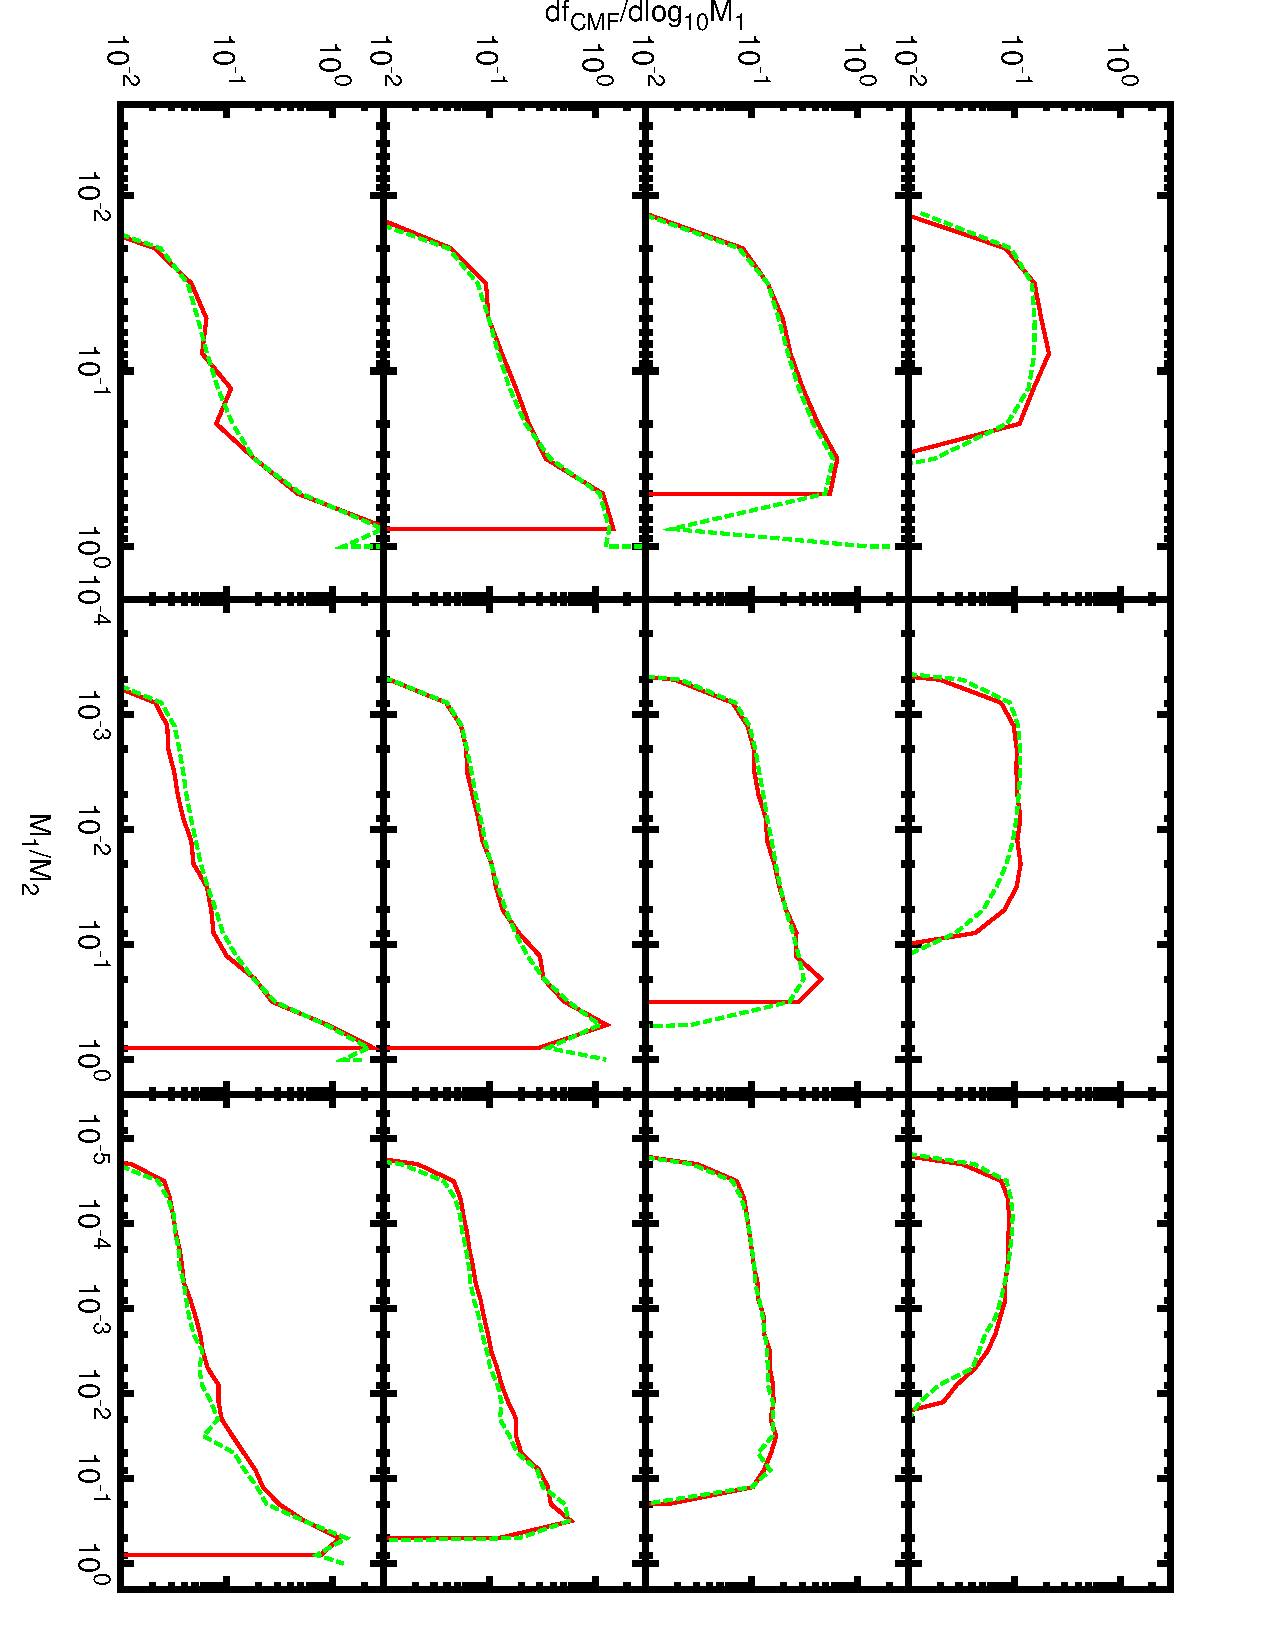
\includegraphics[height=160mm,angle=90]{../plots/progenitorMassFunction.pdf}
 \end{center}
 \caption{Progenitor mass functions at redshifts $z=0.5$, 1, 2 and 4 (bottom to top) for halos of mass $10^{12\pm0.151}$, $10^{13.5\pm0.151}$ and $10^{15\pm0.151}h^{-1}M_\odot$ (left to right) are shown. Green lines are measured from the Millennium Simulation, while red lines are computed using \glc's merger tree building routines (with the \cite{parkinson_generating_2008} branching algorithm and the \cite{cole_hierarchical_2000} tree building algorithm).}
 \label{fig:PCH_Progenitor_MFs}
\end{figure}

\subsubsection{Merger Tree Building}\label{sec:MergerTreeBuildMethod}

Additional methods for merger tree building can be added using the {\tt mergerTreeBuildMethod} directive. The directive should contain a single argument, giving the name of a subroutine to be called to initialize the method. For example, the {\tt Cole2000} method is described by a directive:
\begin{verbatim}
 !# <mergerTreeBuildMethod>
 !#  <unitName>Merger_Tree_Build_Cole2000_Initialize</unitName>
 !# </mergerTreeBuildMethod>
\end{verbatim}
Here, {\tt Merger\_Tree\_Build\_Cole2000\_Initialize} is the name of a subroutine which will be called to initialize the method. The initialization subroutine must have the following form:
\begin{verbatim}
 subroutine Method_Initialize(mergerTreeBuildMethod,Merger_Tree_Build)
    type(varying_string),          intent(in)    :: mergerTreeBuildMethod
    procedure(),          pointer, intent(inout) :: Merger_Tree_Build
    
    if (mergerTreeBuildMethod == 'myMethod') then
       Merger_Tree_Build => My_Do_Tabulate
       .
       .
       .
    end if
    return
  end subroutine Method_Initialize
\end{verbatim}
where {\tt myMethod} is the name of this method as will be specified by the {\tt mergerTreeBuildMethod} input parameter. The procedure pointer {\tt Merger\_Tree\_Build} must build and return a merger tree given the a base node as described below. The initialization subroutine should perform any other tasks required to initialize the module (such as reading parameters etc.).

\begin{verbatim}
  subroutine Merger_Tree_Build_Do(thisTree)
    type(mergerTree), intent(inout) :: thisTree
    .
    .
    .
    return
  end subroutine Merger_Tree_Build_Do
\end{verbatim}
and should return a full merger tree in {\tt thisTree} built from the base node which will already be set in {\tt thisTree}. The tree must have at least masses, times and parent/child/sibling links created. Other properties (e.g. spins) can be optionally included also.

Currently defined merger tree building methods are:
\begin{description}
 \item [{\tt Cole2000}] Uses the \cite{cole_hierarchical_2000} merger tree building algorithm.
\end{description}

\subsubsection{Merger Tree Construction}\label{sec:MergerTreeConstruction}

Additional methods for merger tree construction can be added using the {\tt mergerTreeConstructMethod} directive. The directive should contain a single argument, giving the name of a subroutine to be called to initialize the method. For example, the {\tt build} method is described by a directive:
\begin{verbatim}
 !# <mergerTreeConstructMethod>
 !#  <unitName>Merger_Tree_Build_Initialize</unitName>
 !# </mergerTreeConstructMethod>
\end{verbatim}
Here, {\tt Merger\_Tree\_Build\_Initialize} is the name of a subroutine which will be called to initialize the method. The initialization subroutine must have the following form:
\begin{verbatim}
   subroutine Method_Initialize(mergerTreeConstructMethod,Merger_Tree_Construct)
    type(varying_string),          intent(in)    :: mergerTreeConstructMethod
    procedure(),          pointer, intent(inout) :: Merger_Tree_Construct
    
    if (mergerTreeConstructMethod.eq.'myMethod') then
       Merger_Tree_Construct => My_Do_Tabulate
       .
       .
       .
    end if
    return
  end subroutine Method_Initialize
\end{verbatim}
where {\tt myMethod} is the name of this method as will be specified by the {\tt mergerTreeConstructMethod} input parameter. The procedure pointer {\tt Merger\_Tree\_Construct} must be set to point to a function which returns a fully constructed merger tree as described below. The initialization subroutine should perform any other tasks required to initialize the module (such as reading parameters etc.).

The construction subroutine should have the following form:
\begin{verbatim}
  subroutine Merger_Tree_Construct_Do(thisTree,skipTree)
    type(mergerTree), intent(inout) :: thisTree
    logical,          intent(in)    :: skipTree
    .
    .
    .
    return
  end subroutine Merger_Tree_Construct_Do
\end{verbatim}
and should return a full merger tree in {\tt thisTree}, unless {\tt skipTree} is true, in which case this tree will be skipped (i.e. not evolved or output) and so it suffices to merely allocate the base node---there is no need to create the entire tree (although it is permissible to do so)---and update any internal data (e.g. a count of trees constructed) as required. The tree must have at least masses, times and parent/child/sibling links created. Other properties (e.g. spins) can be optionally included also.

Currently defined merger tree building methods are:
\begin{description}
 \item [{\tt build}] Generates a set of halo masses distributed between {\tt mergerTreeBuildHaloMassMinimum} and {\tt mergerTreeBuildHaloMassMaximum} (with {\tt mergerTreeBuildTreesPerDecade} halos per decade of mass) at redshift {\tt mergerTreeBuildTreesBaseRedshift} and then uses the selected merger tree build method (see \S\ref{sec:MergerTreeBuildMethod}) to build trees from these base nodes;
 \item [{\tt read}] Reads merger tree data from an HDF5 file (see \S\ref{sec:MergerTreeFiles}). The file to read is specified by the {\tt [mergerTreeReadFileName]} parameter.
 \item [{\tt smoothAccretion}] Constructs a branchless merger tree with a smooth accretion history based on the fitting formula of \cite{wechsler_concentrations_2002}. See \S\ref{sec:SmoothAccretion} for details.
\end{description}

\subsubsection{Population III Supernovae}

Additional methods for Population III supernovae can be added using the {\tt supernovaePopIIIMethod} directive. The directive should contain a single argument, giving the name of a subroutine to be called to initialize the method. For example, the {\tt Heger + Woosley} method is described by a directive:
\begin{verbatim}
  !# <supernovaePopIIIMethod>
  !#  <unitName>Supernovae_Population_III_HegerWoosley_Initialize</unitName>
  !# </supernovaePopIIIMethod>
\end{verbatim}
Here, {\tt Supernovae\_Population\_III\_HegerWoosley\_Initialize} is the name of a subroutine which will be called to initialize the method. The initialization subroutine must have the following form:
\begin{verbatim}
  subroutine Method_Initialize(supernovaePopIIIMethod,SNePopIII_Cumulative_Energy_Get)
    implicit none
    type(varying_string),          intent(in)    :: supernovaePopIIIMethod
    procedure(),          pointer, intent(inout) :: SNePopIII_Cumulative_Energy_Get
    
    if (supernovaePopIIIMethod == 'myMethod') then
       SNePopIII_Cumulative_Energy_Get => My_SNePopIII_Cumulative_Energy_Get
       .
       .
       .
    end if
    return
  end subroutine Method_Initialize
\end{verbatim}
where {\tt myMethod} is the name of this method as will be specified by the {\tt supernovaePopIIIMethod} input parameter. The procedure pointer {\tt SNePopIII\_Cumulative\_Energy\_Get} must be set to point to a function which returns the cumulative energy input from Population III supernovae as described below. The initialization subroutine should perform any other tasks required to initialize the module (such as reading parameters etc.).

The functions must have the form:
\begin{verbatim}
   double precision function PopIII_Cumulative_Energy(initialMass,age,metallicity)
    implicit none
    double precision, intent(in) :: initialMass,age,metallicity
    .
    .
    .
    return
   end function PopIII_Cumulative_Energy 
\end{verbatim}
This function must return the cumulative energy (in $M_\odot$ (km/s)$^2$) from Population III supernovae resulting from a star with given {\tt initialMass} and {\tt metallicity} after a time {\tt age}.

Currently defined population III supernovae methods are:
\begin{description}
 \item [{\tt Heger + Woosley}] Computes the energy input from the pair-instability results of \cite{heger_nucleosynthetic_2002}.
\end{description}

\subsubsection{Primordial Power Spectrum}

Additional methods for the primordial power spectrum can be added using the {\tt powerSpectrumMethod} directive. The directive should contain a single argument, giving the name of a subroutine to be called to initialize the method. For example, the {\tt power law} method is described by a directive:
\begin{verbatim}
  !# <powerSpectrumMethod>
  !#  <unitName>CDM_Primordial_Power_Spectrum_Power_Law_Initialize</unitName>
  !# </powerSpectrumMethod>
\end{verbatim}
Here, {\tt CDM\_Primordial\_Power\_Spectrum\_Power\_Law\_Initialize} is the name of a subroutine which will be called to initialize the method. The initialization subroutine must have the following form:
\begin{verbatim}
  subroutine Method_Initialize(powerSpectrumMethod,Power_Spectrum_Tabulate)
    implicit none
    type(varying_string),          intent(in)    :: powerSpectrumMethod
    procedure(),          pointer, intent(inout) :: Power_Spectrum_Tabulate
    
    if (powerSpectrumMethod.eq.'myMethod') then
       Power_Spectrum_Tabulate => My_Do_Tabulate
       .
       .
       .
    end if
    return
  end subroutine Method_Initialize
\end{verbatim}
where {\tt myMethod} is the name of this method as will be specified by the {\tt powerSpectrumMethod} input parameter. The procedure pointer {\tt Power\_Spectrum\_Tabulate} must be set to point to a subroutine which tabulates the power spectrum as described below. The initialization subroutine should perform any other tasks required to initialize the module (such as reading parameters etc.).

The tabulation subroutine must have the form:
\begin{verbatim}
   subroutine Power_Spectrum_Tabulate(wavenumber,powerSpectrumNumberPoints,powerSpectrumLogWavenumber,powerSpectrumLogP)
    implicit none
    double precision,                            intent(in)    :: wavenumber
    double precision, allocatable, dimension(:), intent(inout) :: powerSpectrumLogWavenumber,powerSpectrumLogP
    integer,                                     intent(out)   :: powerSpectrumNumberPoints
    .
    .
    .
    return
   end subroutine Power_Spectrum_Tabulate
\end{verbatim}
The subroutine must tabulate the natural log of the power spectrum in array {\tt powerSpectrumLogP()} as a function of the natural log of wavenumber {\tt powerSpectrumLogWavenumber()} (these arrays must be allocated to the correct size, and may be prevously allocated, therefore requiring a deallocation). The number of tabulated points should be returned in {\tt powerSpectrumNumberPoints}. The subroutine should ensure that the currently requested {\tt wavenumber} is within the range of the tabulated function (preferably with some buffer).

Currently defined power spectrum methods are:
\begin{description}
 \item [{\tt power law}] The power spectrum is assumed to be a power law, possibly with a running index. It is defined by
\begin{equation}
 P(k)\propto k^{n_{\rm s} + \ln(k/k_{\rm ref}) [\d n /\d\ln k]},
\end{equation}
where the parameters are specified by input parameters $n_{\rm s}\equiv${\tt powerSpectrumIndex}, $k_{\rm ref}\equiv${\tt powerSpectrumReferenceWavenumber} and $\d n / \d \ln k \equiv${\tt powerSpectrumRunning}.
\end{description}

\subsubsection{Satellite Merging Mass Movements}

Additional methods for the satellite merging mass movements can be added using the {\tt satelliteMergingMassMovementsMethod} directive. The directive should contain a single argument, giving the name of a subroutine to be called to initialize the method. For example, the {\tt simple} method is described by a directive:
\begin{verbatim}
 !# <satelliteMergingMassMovementsMethod>
 !#  <unitName>Satellite_Merging_Mass_Movements_Simple_Initialize</unitName>
 !# </satelliteMergingMassMovementsMethod>
\end{verbatim}
Here, {\tt Satellite\_Merging\_Mass\_Movements\_Simple\_Initialize} is the name of a subroutine which will be called to initialize the method. The initialization subroutine must have the following form:
\begin{verbatim}
  subroutine Method_Initialize(satelliteMergingMassMovementsMethod,Satellite_Merging_Mass_Movement_Get)
    implicit none
    type(varying_string),          intent(in)    :: satelliteMergingMassMovementsMethod
    procedure(),          pointer, intent(inout) :: Satellite_Merging_Mass_Movement_Get
    
    if (satelliteMergingMassMovementsMethod == 'simple') Satellite_Merging_Mass_Movement_Get => My_Method_Get
    return
  end subroutine Method_Initialize
\end{verbatim}
where {\tt myMethod} is the name of this method as will be specified by the {\tt satelliteMergingMassMovementsMethod} input parameter. The procedure pointer {\tt Satellite\_Merging\_Mass\_Movement\_Get} must be set to point to a function which sets the mass movement descriptors as described below. The initialization subroutine should perform any other tasks required to initialize the module (such as reading parameters etc.).

The mass movement subroutine must have the form:
\begin{verbatim}
  subroutine My_Method_Get(thisNode,gasMovesTo,starsMoveTo,hostGasMovesTo,hostStarsMoveTo)
    implicit none
    type(treeNode), intent(inout), pointer  :: thisNode
    integer,        intent(out)             :: gasMovesTo,starsMoveTo,hostGasMovesTo,hostStarsMoveTo
    .
    .
    .
    return
  end subroutine My_Method_Get
\end{verbatim}
The subroutine must return values for each of the ``{\tt MoveTo}'' descriptors to specify where stars and gas from {\tt thisNode} and {\tt thisNode}'s host node should move to in the host. Allowed values are:
\begin{description}
 \item [{\tt movesToDisk}] The material in question moves to the disk of the host node;
 \item [{\tt movesToSpheroid}] The material in question moves to the spheroid of the host node;
 \item [{\tt doesNotMove}] The material in question does not move (allowed only for host node descriptors).
\end{description}

Currently defined satellite merger mass movement methods are:
\begin{description}
 \item [{\tt simple}] If the baryonic mass of the satellite exceeds a fraction {\tt majorMergerMassRatio} of the baryonic mass of the host then all material is moved to the spheroid of the host. Otherwise, satellite gas moves to the host disk, satellite stars move to the host spheroid and host material does not move.
\end{description}

\subsubsection{Satellite Merging Remnant Sizes}\label{sec:satelliteMergerMassMovementMethod}

Additional methods for the satellite merging remnant sizes can be added using the {\tt satelliteMergingRemnantSizeMethod} directive. The directive should contain a single argument, giving the name of a subroutine to be called to initialize the method. For example, the {\tt Cole2000} method is described by a directive:
\begin{verbatim}
 !# <satelliteMergingRemnantSizeMethod>
 !#  <unitName>Satellite_Merging_Remnant_Sizes_Cole2000_Initialize</unitName>
 !# </satelliteMergingRemnantSizeMethod>
\end{verbatim}
Here, {\tt Satellite\_Merging\_Remnant\_Sizes\_Cole2000\_Initialize} is the name of a subroutine which will be called to initialize the method. The initialization subroutine must have the following form:
\begin{verbatim}
  subroutine Method_Initialize(satelliteMergingRemnantSizeMethod,Satellite_Merging_Remnant_Size_Do)
    implicit none
    type(varying_string),          intent(in)    :: satelliteMergingRemnantSizeMethod
    procedure(),          pointer, intent(inout) :: Satellite_Merging_Remnant_Size_Do
    
    if (satelliteMergingRemnantSizeMethod == 'myMethod') Satellite_Merging_Remnant_Size_Do => My_Method_Do
    return
  end subroutine Method_Initialize
\end{verbatim}
where {\tt myMethod} is the name of this method as will be specified by the {\tt satelliteMergingRemnantSizeMethod} input parameter. The procedure pointer {\tt Satellite\_Merging\_Remnant\_Size\_Do} must be set to point to a function which computes the size of the merger remnant and stores the properties (e.g. radius, circular velocity and specific angular momentum at the half-mass radius) of the \emph{host} node. The initialization subroutine should perform any other tasks required to initialize the module (such as reading parameters etc.).

The remnant size subroutine must have the form:
\begin{verbatim}
  subroutine My_Method_Do(thisNode)
    implicit none
    type(treeNode), intent(inout), pointer  :: thisNode
    .
    .
    .
    return
  end subroutine My_Method_Do
\end{verbatim}
The subroutine must compute the properties of the merger remnant. Typically these are stored in the {\tt Satellite\_Merging\_Remnant\_Sizes\_Properties} module for later retrieval by the appropriate component.

Currently defined satellite merger remnant size methods are:
\begin{description}
 \item [{\tt null}] This is a null method which does nothing. It is useful for runs where no baryonic components are included (e.g. for studying dark matter only).
 \item [{\tt Cole2000}] Implements the algorithm of \cite{cole_hierarchical_2000} to compute the remnant size. The orbital energy assumed can be adjusted using the {\tt mergerRemnantSizeOrbitalEnergy} parameter, which is equivalent to the $f_{\rm orbit}$ parameter of \cite{cole_hierarchical_2000}.
\end{description}

\subsubsection{Satellite Merging Timescales}

Additional methods for the satellite merging timescales can be added using the {\tt satelliteMergingMethod} directive. The directive should contain a single argument, giving the name of a subroutine to be called to initialize the method. For example, the {\tt Lacey-Cole} method is described by a directive:
\begin{verbatim}
  !# <satelliteMergingMethod>
  !#  <unitName>Satellite_Time_Until_Merging_Lacey_Cole_Initialize</unitName>
  !# </satelliteMergingMethod>
\end{verbatim}
Here, {\tt Satellite\_Time\_Until\_Merging\_Lacey\_Cole\_Initialize} is the name of a subroutine which will be called to initialize the method. The initialization subroutine must have the following form:
\begin{verbatim}
  subroutine Method_Initialize(satelliteMergingMethod,Satellite_Time_Until_Merging)
    implicit none
    type(varying_string),          intent(in)    :: satelliteMergingMethod
    procedure(),          pointer, intent(inout) :: Satellite_Time_Until_Merging
    
    if (satelliteMergingMethod == 'myMethod') Satellite_Time_Until_Merging => My_Method_Procedure
    return
  end subroutine Method_Initialize
\end{verbatim}
where {\tt myMethod} is the name of this method as will be specified by the {\tt satelliteMergingMethod} input parameter. The procedure pointer {\tt Satellite\_Time\_Until\_Merging} must be set to point to a function which returns the time until merging as described below. The initialization subroutine should perform any other tasks required to initialize the module (such as reading parameters etc.).

The merging timescale function must have the form:
\begin{verbatim}
 double precision function Satellite_Time_Until_Merging(thisNode)
    implicit none
    type(treeNode),   pointer, intent(inout) :: thisNode
    .
    .
    .
    return
 end function Satellite_Time_Until_Merging
\end{verbatim}
The function must return the merging timescale for {\tt thisNode} orbitting in {\tt thisNode\%parentNode} in units of Gyr.

Currently defined satellite virial orbit methods are:
\begin{description}
 \item [\hyperlink{satellites.merging.dynamical_friction.timescale.Lacey-Cole.F90:dynamical_friction_lacey_cole:satellite_time_until_merging_lacey_cole}{{\tt Lacey-Cole}}] Computes the merging timescale using the method of \cite{lacey_merger_1993}.
 \item [\hyperlink{satellites.merging.dynamical_friction.timescale.Jiang2008.F90:dynamical_friction_jiang2008:satellite_time_until_merging_jiang2008}{{\tt Jiang2008}}] Computes the merging timescale using the method of \cite{jiang_fitting_2008}.
 \item [\hyperlink{satellites.merging.dynamical_friction.timescale.Boylan-Kolchin2008.F90:dynamical_friction_boylankolchin2008:satellite_time_until_merging_boylankolchin2008}{{\tt BoylanKolchin2008}}] Computes the merging timescale using the method of \cite{boylan-kolchin_dynamical_2008}.
\end{description}

\subsubsection{Satellite Virial Orbits}

Additional methods for the satellite virial orbits (i.e. orbital parameters at virial radius crossing) can be added using the {\tt virialOrbitsMethod} directive. The directive should contain a single argument, giving the name of a subroutine to be called to initialize the method. For example, the {\tt Benson2005} method is described by a directive:
\begin{verbatim}
  !# <virialOrbitsMethod>
  !#  <unitName>Virial_Orbital_Parameters_Benson2005_Initialize</unitName>
  !# </virialOrbitsMethod>
\end{verbatim}
Here, {\tt Virial\_Orbital\_Parameters\_Benson2005\_Initialize} is the name of a subroutine which will be called to initialize the method. The initialization subroutine must have the following form:
\begin{verbatim}
  subroutine Method_Initialize(virialOrbitsMethod,Virial_Orbital_Parameters_Get)
    implicit none
    type(varying_string),          intent(in)    :: virialOrbitsMethod
    procedure(),          pointer, intent(inout) :: Virial_Orbital_Parameters_Get
    
    if (virialOrbitsMethod.eq.'myMethod') Virial_Orbital_Parameters_Get => My_Method_Procedure
    return
  end subroutine Method_Initialize
\end{verbatim}
where {\tt myMethod} is the name of this method as will be specified by the {\tt virialOrbitsMethod} input parameter. The procedure pointer {\tt Virial\_Orbital\_Parameters\_Get} must be set to point to a subroutine which returns orbital parameters as described below. The initialization subroutine should perform any other tasks required to initialize the module (such as reading parameters etc.).

The orbital parameter subroutine must have the form:
\begin{verbatim}
  subroutine Virial_Orbital_Parameters(thisNode,acceptUnboundOrbits,velocityRadial,velocityTangential,angularMomentum&
       &,orbitalEnergy,eccentricity,semimajorAxis)
    implicit none
    type(treeNode),   intent(inout), pointer  :: thisNode
    logical,          intent(in)              :: acceptUnboundOrbits
    double precision, intent(out),   optional :: velocityRadial,velocityTangential,angularMomentum,orbitalEnergy,eccentricity&
         &,semimajorAxis

    return
  end subroutine Virial_Orbital_Parameters
\end{verbatim}
The subroutine must return orbital parameters for {\tt thisNode} orbitting in {\tt thisNode\%parentNode}, for whichever of the arguments are present in the subroutine call. If {\tt acceptUnboundOrbits} is true, then unbound orbits may be returned, otherwise, the routine must ensure that the returned orbit is bound. Velocities should be return in units of km/s, lengthscales in units of Mpc.

Currently defined satellite virial orbit methods are:
\begin{description}
 \item [\hyperlink{satellites.merging.virial_orbits.Benson2005.F90:virial_orbits_benson2005:virial_orbital_parameters_benson2005}{{\tt Benson2005}}] The orbital parameters are select from the distribution found by \cite{benson_orbital_2005}.
 \item [\hyperlink{satellites.merging.virial_orbits.Wetzel2010.F90:virial_orbits_wetzel2010:virial_orbital_parameters_wetzel2010}{{\tt Wetzel2010}}] The orbital parameters are select from the distribution found by \cite{wetzel_orbits_2010}.
\end{description}

\subsubsection{Star Formation Feedback in Disks/Spheroids}

Additional methods for computing feedback from star formation in disks/spheroids can be added using the {\tt starFormationFeedback[Disks|Spheroids]Method} directive. The directive should contain a single argument, giving the name of a subroutine to be called to initialize the method. For example, the {\tt power law} method is described by a directive:
\begin{verbatim}
 !# <starFormationFeedbackSpheroidsMethod>
 !#  <unitName>Star_Formation_Feedback_Spheroids_Power_Law_Initialize</unitName>
 !# </starFormationFeedbackSpheroidsMethod>
\end{verbatim}
Here, {\tt Star\_Formation\_Feedback\_Spheroids\_Power\_Law\_Initialize} is the name of a subroutine which will be called to initialize the method. The initialization subroutine must have the following form:
\begin{verbatim}
  subroutine Method_Initialize(starFormationFeedbackDisksMethod,Star_Formation_Feedback_Disk_Outflow_Rate_Get)
    implicit none
    type(varying_string),          intent(in)    :: starFormationFeedbackDisksMethod
    procedure(),          pointer, intent(inout) :: Star_Formation_Feedback_Disk_Outflow_Rate_Get
    
    if (starFormationFeedbackDisksMethod == 'myMethod') Star_Formation_Feedback_Disk_Outflow_Rate_Get => My_Star_Formation_Feedback_Disk_Outflow_Rate_Get
    return
  end subroutine Method_Initialize
\end{verbatim}
where {\tt myMethod} is the name of this method as will be specified by the {\tt starFormationFeedback[Disks|Spheroids]Method} input parameter. The procedure pointer {\tt Star\_Formation\_Feedback\_Disk\_Outflow\_Rate\_Get} (or {\tt Star\_Formation\_Feedback\_Spheroid\_Outflow\_Rate\_Get} for the spheroid case) must be set to point to a function which returns the mass outflow rate due to star formation as described below. The initialization subroutine should perform any other tasks required to initialize the module (such as reading parameters etc.).

The outflow rate function must have the form:
\begin{verbatim}
 double precision function Star_Formation_Feedback_Outflow_Rate_Get(thisNode,starFormationRate,energyInputRate)
    implicit none
    type(treeNode),   intent(inout), pointer :: thisNode
    double precision, intent(in)             :: starFormationRate,energyInputRate
    .
    .
    .
    return
 end function Star_Formation_Feedback_Outflow_Rate_Get
\end{verbatim}
The function must return the mass outflow rate (in $M_\odot$ Gyr$^{-1}$) for {\tt thisNode}.

Currently defined star formation feedback methods are:
\begin{description}
 \item [\hyperlink{star_formation.feedback.spheroids.power_law.F90:star_formation_feedback_spheroids_power_law:star_formation_feedback_spheroid_outflow_rate_power_law}{{\tt power law}}] The outflow rate is given by
\begin{equation}
 \dot{M}_{\rm outflow} = \left({V_{\rm outflow} \over V}\right)^{\alpha_{\rm outflow}} {\dot{E} \over E_{\rm canonical}},
\end{equation}
where $V_{\rm outflow}=${\tt [disk|spheroid]OutflowVelocity} (in km/s) and $\alpha_{\rm outflow}=${\tt [disk|spheroid]OutflowVelocity} are input parameters, $V$ is the characteristic velocity of the component, $\dot{E}$ is the rate of energy input from stellar populations and $E_{\rm canonical}$ is the total energy input by a canonical stellar population normalized to $1 M_\odot$ after infinite time.
\end{description}

\subsubsection{Star Formation Timescale in Disks/Spheroids}

Additional methods for computing star formation timescales in disks/spheroids can be added using the {\tt starFormationTimescale[Disks|Spheroids]Method} directive. The directive should contain a single argument, giving the name of a subroutine to be called to initialize the method. For example, the {\tt dynamical time} method is described by a directive:
\begin{verbatim}
 !# <starFormationTimescaleDisksMethod>
 !#  <unitName>Star_Formation_Timescale_Disks_Dynamical_Time_Initialize</unitName>
 !# </starFormationTimescaleDisksMethod>
\end{verbatim}
Here, {\tt Star\_Formation\_Timescale\_Disks\_Dynamical\_Time\_Initialize} is the name of a subroutine which will be called to initialize the method. The initialization subroutine must have the following form:
\begin{verbatim}
  subroutine Method_Initialize(starFormationTimescaleDisksMethod,Star_Formation_Timescale_Disk_Get)
    implicit none
    type(varying_string),          intent(in)    :: starFormationTimescaleDisksMethod
    procedure(),          pointer, intent(inout) :: Star_Formation_Timescale_Disk_Get
    
    if (starFormationTimescaleDisksMethod == 'myMethod') Star_Formation_Timescale_Disk_Get => My_Method_Get_Procedure
    return
  end subroutine Method_Initialize
\end{verbatim}
where {\tt myMethod} is the name of this method as will be specified by the {\tt starFormationTimescale[Disks|Spheroids]Method} input parameter. The procedure pointer {\tt Star\_Formation\_Timescale\_Disk\_Get} (or {\tt Star\_Formation\_Timescale\_Spheroid\_Get} for the spheroid case) must be set to point to a function which returns the timescale for star formation as described below. The initialization subroutine should perform any other tasks required to initialize the module (such as reading parameters etc.).

The star formation timescale function must have the form:
\begin{verbatim}
 double precision function Star_Formation_Timescale_Get(thisNode)
    implicit none
    type(treeNode), intent(in) :: thisNode
    .
    .
    .
    return
 end function Star_Formation_Timescale_Get
\end{verbatim}
The function must return the star formation timescale (in units of Gyr) for {\tt thisNode}.

Currently defined star formation timescale methods are:
\begin{description}
 \item [\hyperlink{star_formation.timescales.disks.dynamical_time.F90:star_formation_timescale_disks_dynamical_time:star_formation_timescale_disk_dynamical_time}{{\tt dynamical time}}]  The timescale is given by
\begin{equation}
 \tau_\star = \epsilon_\star^{-1} \tau_{\rm dynamical, [disk|spheroid]} \left( {V_{\rm [disk|spheroid]} \over 200\hbox{km/s}} \right)^{\alpha_\star},
\end{equation}
where $\epsilon_\star$(={\tt starFormation[Disk|Spheroid]Efficiency}) is a star formation efficiency and $\alpha_\star$(={\tt starFormation[Disk|Spheroid]VelocityExponent}) controls the scaling with velocity. Note that $\tau_{\rm dynamical,[disk|spheroid]}=R_{\rm [disk|spheroid]}/V_{\rm [disk|spheroid]}$ where the radius and velocity are whatever characteristic values returned by the disk/spheroid method. This scaling is functionally similar to that adopted by \cite{cole_hierarchical_2000}, but that they specifically used the half-mass radius and circular velocity at that radius.
\end{description}

\subsubsection{Stellar Astrophysics}

Additional methods for stellar astrophysical properties can be added using the {\tt stellarAstrophysicsMethod} directive. The directive should contain a single argument, giving the name of a subroutine to be called to initialize the method. For example, the {\tt file} method is described by a directive:
\begin{verbatim}
  !# <stellarAstrophysicsMethod>
  !#  <unitName>Stellar_Astrophysics_File_Initialize</unitName>
  !# </stellarAstrophysicsMethod>
\end{verbatim}
Here, {\tt Stellar\_Astrophysics\_File\_Initialize} is the name of a subroutine which will be called to initialize the method. The initialization subroutine must have the following form:
\begin{verbatim}
  subroutine Method_Initialize(stellarAstrophysicsMethod,Star_Ejected_Mass_Get,Star_Initial_Mass_Get,Star_Metal_Yield_Mass_Get,Star_Lifetime_Get)
    implicit none
    type(varying_string),          intent(in)    :: stellarAstrophysicsMethod
    procedure(),          pointer, intent(inout) :: Star_Ejected_Mass_Get,Star_Initial_Mass_Get,Star_Metal_Yield_Mass_Get,Star_Lifetime_Get
    
    if (stellarAstrophysicsMethod == 'myMethod') then
      Star_Ejected_Mass_Get     => My_Star_Ejected_Mass
      Star_Initial_Mass_Get     => My_Star_Initial_Mass
      Star_Metal_Yield_Mass_Get => My_Star_Metal_Yield_Mass
      Star_Lifetime_Get         => My_Star_Lifetime
    end if
    return
  end subroutine Method_Initialize
\end{verbatim}
where {\tt myMethod} is the name of this method as will be specified by the {\tt stellarAstrophysicsMethod} input parameter. The procedure pointers must be set to point to functions which return stellar properties as described below. The initialization subroutine should perform any other tasks required to initialize the module (such as reading parameters etc.).

The ejected mass and lifetime functions must have the form:
\begin{verbatim}
 double precision function Star_Property(initialMass,metallicity)
    implicit none
    double precision, intent(in) :: initialMass,metallicity
    .
    .
    .
    return
 end function Star_Property
\end{verbatim}
These functions must return the total ejected mass (in $M_\odot$), total metal yield (in $M_\odot$) and lifetime (in Gyr) for a star of the specified {\tt initialMass} and {\tt metallicity}.

The metal yield function must have the form:
\begin{verbatim}
 double precision function Star_Metal_Yield(initialMass,metallicity,atomIndex)
    implicit none
    double precision, intent(in)           :: initialMass,metallicity
    integer,          intent(in), optional :: atomIndex
    .
    .
    .
    return
 end function Star_Property
\end{verbatim}
This function must return the yield (in $M_\odot$) of the element identified by {\tt atomIndex} (as returned by the \hyperlink{atomic.data.F90:atomic_data:atom_lookup}{{\tt Atom\_Lookup()}} function from the \hyperlink{atomic.data.F90:atomic_data}{{\tt Atomic\_Data}} module) if present, or total metal yield otherwise for a star of the specified {\tt initialMass} and {\tt metallicity}.

The initial mass function must have the form:
\begin{verbatim}
 double precision function Star_Initial_Mass(lifetime,metallicity)
    implicit none
    double precision, intent(in) :: lifetime,metallicity
    .
    .
    .
    return
 end function Star_Initial_Mass
\end{verbatim}
and should return the initial mass (in $M_\odot$) of a star of given {\tt lifetime} (specified in Gyr) and {\tt metallicity}.

Currently defined stellar astrophysics methods are:
\begin{description}
 \item [{\tt file}] Stellar properties are read from an XML file and interpolated. The structure of the XML file is described in \S\ref{sec:StellarAstrophysicsFile}.
\end{description}

\subsubsection{Stellar Population Properties}

Additional methods for computing properties of stellar populations can be added using the {\tt stellarPopulationPropertiesMethod} directive. The directive should contain a single argument, giving the name of a subroutine to be called to initialize the method. For example, the {\tt instantaneous} method is described by a directive:
\begin{verbatim}
 !# <stellarPopulationPropertiesMethod>
 !#  <unitName>Stellar_Population_Properties_Instantaneous_Initialize</unitName>
 !# </stellarPopulationPropertiesMethod>
\end{verbatim}
Here, {\tt Stellar\_Population\_Properties\_Instantaneous\_Initialize} is the name of a subroutine which will be called to initialize the method. The initialization subroutine must have the following form:
\begin{verbatim}
  subroutine Method_Initialize(stellarPopulationPropertiesMethod,Stellar_Population_Properties_Rates_Get,Stellar_Population_Properties_History_Count_Get)
    implicit none
    type(varying_string),          intent(in)    :: stellarPopulationPropertiesMethod
    procedure(),          pointer, intent(inout) :: Stellar_Population_Properties_Rates_Get,Stellar_Population_Properties_History_Count_Get
    
    if (stellarPopulationPropertiesMethod == 'myMethod') then
       Stellar_Population_Properties_Rates_Get         => My_Method_Rates_Get_Procedure
       Stellar_Population_Properties_History_Count_Get => My_Method_History_Count_Get_Procedure
    end if
    return
  end subroutine Method_Initialize
\end{verbatim}
where {\tt myMethod} is the name of this method as will be specified by the {\tt stellarPopulationPropertiesMethod} input parameter. The procedure pointer {\tt Stellar\_Population\_Properties\_Rates\_Get} must be set to point to a subroutine which returns properties of a stellar population as described below, while the {\tt My\_Method\_History\_Count\_Get\_Procedure} procedure pointer must be set to point to a function which returns the number of histories that will be required by this method. The initialization subroutine should perform any other tasks required to initialize the module (such as reading parameters etc.).

The stellar populations properties subroutine must have the form:
\begin{verbatim}
 subroutine Stellar_Population_Properties_Rates(starFormationRate,fuelAbundances,thisNode,thisHistory,stellarMassRate&
       &,stellarAbundancesRates,stellarLuminositiesRates,fuelMassRate,fuelAbundancesRates,energyInputRate)
    implicit none
    implicit none
    double precision,          intent(out)                 :: stellarMassRate,fuelMassRate,energyInputRate
    type(abundancesStructure), intent(out)                 :: stellarAbundancesRates,fuelAbundancesRates
    double precision,          intent(out),   dimension(:) :: stellarLuminositiesRates
    double precision,          intent(in)                  :: starFormationRate
    type(abundancesStructure), intent(in)                  :: fuelAbundances
    type(treeNode),            intent(inout), pointer      :: thisNode
    type(history),             intent(inout)               :: thisHistory
    .
    .
    .
    return
 end subroutine Stellar_Population_Properties_Rates
\end{verbatim}
The subroutine is given the {\tt starFormationRate} (in $M_\odot$ Gyr$^{-1}$) in {\tt thisNode}. Any history information required by this method must be passed in via the {\tt history} argument. Stars are forming from fuel material with composition specified by {\tt fuelAbundances}. The subroutine must return the rates of change of stellar and fuel mass (in $M_\odot$ Gyr$^{-1}$) in {\tt stellarMassRate} and {\tt fuelMassRate} respectively, and the corresponding rates (also in $M_\odot$ Gyr$^{-1}$) of abundance change in {\tt stellarAbundancesRates} and {\tt fuelAbundancesRates} respectively. Finally, it should return rates of change (in $L_{\rm AB}$ Gyr$^{-1}$) of stellar luminosities for all requested output bands in {\tt stellarLuminositiesRates}. Additionally, the rate of energy input from stellar populations must be returned in {\tt energyInputRate}.

The history function function must have the form
\begin{verbatim}
 integer function Stellar_Population_Properties_History_Count()
    implicit none
    .
    .
    return
 end function Stellar_Population_Properties_History_Count
\end{verbatim}
and should return the number of histories that will be required by this method.

Currently defined stellar population properties methods are:
\begin{description}
 \item [\hyperlink{stellar_populations.properties.instantaneous.F90:stellar_population_properties_instantaneous:stellar_population_properties_rates_instantaneous}{{\tt instantaneous}}] Computes stellar population properties using an instantaneous recyclying approximation.
\end{description}

\subsubsection{Stellar Population Spectra}\label{sec:StellarPopulationSpectra}

Additional methods for computing specta of stellar populations can be added using the {\tt stellarPopulationSpectraMethod} directive. The directive should contain a single argument, giving the name of a subroutine to be called to initialize the method. For example, the {\tt Conroy, White \& Gunn} method is described by a directive:
\begin{verbatim}
 !# <stellarPopulationSpectraMethod>
 !#  <unitName>Stellar_Population_Spectra_Conroy_Initialize</unitName>
 !# </stellarPopulationSpectraMethod>
\end{verbatim}
Here, {\tt Stellar\_Population\_Spectra\_Conroy\_Initialize} is the name of a subroutine which will be called to initialize the method. The initialization subroutine must have the following form:
\begin{verbatim}
  subroutine Method_Initialize(stellarPopulationSpectraMethod,Stellar_Population_Spectra_Get,Stellar_Population_Spectrum_Tabulation_Get)
    implicit none
    type(varying_string),          intent(in)    :: stellarPopulationSpectraMethod
    procedure(),          pointer, intent(inout) :: Stellar_Population_Spectra_Get,Stellar_Population_Spectrum_Tabulation_Get
    
    if (stellarPopulationSpectraMethod == 'myMethod') then
        Stellar_Population_Spectra_Get             => My_Method_Spectra_Get
        Stellar_Population_Spectrum_Tabulation_Get => My_Method_Spectrum_Tabulation_Get
    end if
    return
  end subroutine Method_Initialize
\end{verbatim}
where {\tt myMethod} is the name of this method as will be specified by the {\tt stellarPopulationSpectraMethod} input parameter. The procedure pointer {\tt Stellar\_Population\_Spectra\_Get} must be set to point to a function which returns the spectrum of a stellar population as described below while the {\tt Stellar\_Population\_Spectrum\_Tabulation\_Get} pointer must be set to point to a subroutine which returns a tabulation of ages and metallicities on which stellar spectra should be tabulated. The initialization subroutine should perform any other tasks required to initialize the module (such as reading parameters etc.).

The stellar spectra function must have the form:
\begin{verbatim}
  double precision function Stellar_Population_Spectra_Get(abundances,age,wavelength,imfIndex)
    implicit none
    type(abundancesStructure), intent(in) :: abundances
    double precision,          intent(in) :: age,wavelength
    integer,                   intent(in) :: imfIndex
    .
    .
    .
    return
  end function Stellar_Population_Spectra_Get
\end{verbatim}
The function is given the {\tt abundances}, {\tt age} (in Gyr), and {\tt imfIndex} of the stellar population and the {\tt wavelength} (in \AA) at which the spectrum should be computed. The spectrum should be returned in units of $L_\odot$ Hz$^{-1}$.

The tabulation subroutine must have the form:
\begin{verbatim}
  subroutine Stellar_Population_Spectrum_Tabulation(imfIndex,agesCount,metallicitiesCount,age,metallicity)
    implicit none
    integer,          intent(in)                             :: imfIndex
    integer,          intent(out)                            :: agesCount,metallicitiesCount
    double precision, intent(out), allocatable, dimension(:) :: age,metallicity
    .
    .
    .
    return
  end subroutine Stellar_Population_Spectrum_Tabulation
\end{verbatim}
and should return the number of ages and metallicities at which stellar population spectra should be tabualted for the specified \IMF, and should allocate the {\tt age} and {\tt metallicity} arrays appropriately and should fill them with the ages and metallicities at which to tabulate.

Currently defined stellar population properties methods are:
\begin{description}
 \item [\hyperlink{stellar_populations.spectra.Conroy_et_al.F90:stellar_population_spectra_conroy}{{\tt Conroy, White \& Gunn}}] Uses the {\tt FSPS} code of \cite{conroy_propagation_2009} to compute stellar spectra. If necessary, the {\tt FSPS} code will be downloaded, patched and compiled and run to generate spectra. These tabulations are then stored to file for later retrieval.
 \item [\hyperlink{stellar_populations.spectra.file.F90:stellar_population_spectra_file}{{\tt file}}] Stellar spectra for a given \IMF\ are read from the file specified by the {\tt stellarPopulationSpectraForXXXXIMF} where {\tt XXXX} is the name of the \IMF. This should specify an HDF5 file with the following structure:
\begin{verbatim}
 ages                     Dataset {ageCount}
 metallicities            Dataset {metallicityCount}
 spectra                  Dataset {wavelengthCount, ageCount, metallicityCount}
 wavelengths              Dataset {wavelengthCount}
\end{verbatim}
where the datasets contain the tabulated ages (in Gyr), metallicities (logarithmic, relative to Solar), wavelengths (in \AA) and spectra (in $L_\odot$ Hz$^{-1}$).
\end{description}

\subsubsection{Stellar Population Spectra Postprocessing}

Additional methods for postprocessing specta of stellar populations can be added using the {\tt stellarPopulationSpectraPostprocessMethod} directive. The directive should contain a single argument, giving the name of a subroutine to be called to initialize the method. For example, the {\tt Meiksin2006} method is described by a directive:
\begin{verbatim}
 !# <stellarPopulationSpectraPostprocessMethod>
 !#  <unitName>Stellar_Population_Spectra_Postprocess_Meiksin2006_Initialize</unitName>
 !# </stellarPopulationSpectraPostprocessMethod>
\end{verbatim}
Here, {\tt Stellar\_Population\_Spectra\_Postprocess\_Meiksin2006\_Initialize} is the name of a subroutine which will be called to initialize the method. The initialization subroutine must have the following form:
\begin{verbatim}
  subroutine Method_Initialize(stellarPopulationSpectraPostprocessMethod,Stellar_Population_Spectra_Postprocess_Get)
    implicit none
    type(varying_string),          intent(in)    :: stellarPopulationSpectraPostprocessMethod
    procedure(),          pointer, intent(inout) :: Stellar_Population_Spectra_Postprocess_Get
    
    if (stellarPopulationSpectraPostprocessMethod == 'myMethod') then
        Stellar_Population_Spectra_Postprocess_Get => My_Method_Postprocess_Get
    end if
    return
  end subroutine Method_Initialize
\end{verbatim}
where {\tt myMethod} is the name of this method as will be specified by the {\tt stellarPopulationSpectraPostprocessMethod} input parameter. The procedure pointer {\tt Stellar\_Population\_Spectra\_Postprocess\_Get} must be set to point to a function which returns a multiplicative factor by which stellar spectra will be scaled. The initialization subroutine should perform any other tasks required to initialize the module (such as reading parameters etc.).

The stellar spectra postprocessing function must have the form:
\begin{verbatim}
  double precision function Stellar_Population_Spectra_Postprocess_Get(wavelength,redshift)
    implicit none
    double precision, intent(in) :: wavelength,redshift
    .
    .
    .
    return
  end function Stellar_Population_Spectra_Postprocess_Get
\end{verbatim}
The function is given the rest-frame {\tt wavelength} (in \AA) and the {\tt redshift} of the radiation and should return a multiplicative factor by which the spectrum will be scaled.

Currently defined stellar population postprocessing methods are:
\begin{description}
\item [\hyperlink{stellar_populations.spectra.postprocess.Meiksin2006.F90:stellar_population_spectra_postprocess_meiksin2006}{{\tt Meiksin2006}}] Postprocesses spectra through absorption by the \IGM\ using the results of \cite{meiksin_colour_2006}.
\item [\hyperlink{stellar_populations.spectra.postprocess.Madau1995.F90:stellar_population_spectra_postprocess_madau1995}{{\tt Madau1995}}] Postprocesses spectra through absorption by the \IGM\ using the results of \cite{madau_radiative_1995}.
\item [\hyperlink{stellar_populations.spectra.postprocess.null.F90:stellar_population_spectra_postprocess_null}{{\tt null}}] Performs no postprocessing.
\end{description}

\subsubsection{Stellar Feedback}

Additional methods for stellar feedback can be added using the {\tt stellarFeedbackMethod} directive. The directive should contain a single argument, giving the name of a subroutine to be called to initialize the method. For example, the {\tt standard} method is described by a directive:
\begin{verbatim}
  !# <stellarFeedbackMethod>
  !#  <unitName>Stellar_Feedback_Standard_Initialize</unitName>
  !# </stellarFeedbackMethod>
\end{verbatim}
Here, {\tt Stellar\_Feedback\_Standard\_Initialize} is the name of a subroutine which will be called to initialize the method. The initialization subroutine must have the following form:
\begin{verbatim}
  subroutine Method_Initialize(stellarFeedbackMethod,Stellar_Feedback_Cumulative_Energy_Input_Get)
    implicit none
    type(varying_string),          intent(in)    :: stellarFeedbackMethod
    procedure(),          pointer, intent(inout) :: Stellar_Feedback_Cumulative_Energy_Input_Get
    
    if (stellarFeedbackMethod == 'myMethod') then
       Stellar_Feedback_Cumulative_Energy_Input_Get => My_Stellar_Feedback_Cumulative_Energy_Input_Get
       .
       .
       .
    end if
    return
  end subroutine Method_Initialize
\end{verbatim}
where {\tt myMethod} is the name of this method as will be specified by the {\tt stellarFeedbackMethod} input parameter. The procedure pointer {\tt Stellar\_Feedback\_Cumulative\_Energy\_Input\_Get} must be set to point to a function which returns the cumulative energy input from stars as described below. The initialization subroutine should perform any other tasks required to initialize the module (such as reading parameters etc.).

The function must have the form:
\begin{verbatim}
   double precision function Stellar_Feedback_Cumulative_Energy_Input(initialMass,age,metallicity)
    implicit none
    double precision, intent(in) :: initialMass,age,metallicity
    .
    .
    .
    return
   end function Stellar_Feedback_Cumulative_Energy_Input 
\end{verbatim}
The function must return the cumulative energy input (in $M_\odot$ (km/s)$^2$ from stars of given {\tt initialMass} and {\tt metallicity} after a time {\tt age}.

Currently defined stellar feedback methods are:
\begin{description}
 \item [{\tt standard}] This method assumes that the energy input has contributions from stellar winds, Type Ia, Type II and Population III supernovae. The minimum mass required for a star to produce a Type II supernova is specified via {\tt initialMassForSupernovaeTypeII} (in $M_\odot$), while the energy per Type II or Ia supernova is specified via {\tt supernovaEnergy} (in ergs).
\end{description}

\subsubsection{Stellar Tracks}

Additional methods for stellar tracks can be added using the {\tt stellarTracksMethod} directive. The directive should contain a single argument, giving the name of a subroutine to be called to initialize the method. For example, the {\tt file} method is described by a directive:
\begin{verbatim}
  !# <stellarTracksMethod>
  !#  <unitName>Stellar_Tracks_Initialize_File</unitName>
  !# </stellarTracksMethod>
\end{verbatim}
Here, {\tt Stellar\_Tracks\_Initialize\_File} is the name of a subroutine which will be called to initialize the method. The initialization subroutine must have the following form:
\begin{verbatim}
  subroutine Method_Initialize(stellarTracksMethod,Stellar_Luminosity_Get,Stellar_Effective_Temperature_Get)
    implicit none
    type(varying_string),          intent(in)    :: stellarTracksMethod
    procedure(),          pointer, intent(inout) :: Stellar_Luminosity_Get,Stellar_Effective_Temperature_Get
    
    if (stellarTracksMethod == 'myMethod') then
       Stellar_Luminosity_Get            => My_Stellar_Luminosity_Get
       Stellar_Effective_Temperature_Get => My_Stellar_Effective_Temperature_Get
       .
       .
       .
    end if
    return
  end subroutine Method_Initialize
\end{verbatim}
where {\tt myMethod} is the name of this method as will be specified by the {\tt stellarTracksMethod} input parameter. The procedure pointers {\tt Stellar\_Luminosity\_Get} and {\tt Stellar\_Effective\_Temperature\_Get} must be set to point to functions which return the luminosity and effective temperatures of stars as described below. The initialization subroutine should perform any other tasks required to initialize the module (such as reading parameters etc.).

The functions must have the form:
\begin{verbatim}
   double precision function Stellar_Tracks_Function(initialMass,age,metallicity)
    implicit none
    double precision, intent(in) :: initialMass,age,metallicity
    .
    .
    .
    return
   end function Stellar_Tracks_Function 
\end{verbatim}
The luminosity function must return the bolometric luminosity (in $L_\odot$) of a star of given {\tt initialMass} and {\tt metallicity} after a time {\tt age}. The effective temperature function should give the effective temperature (in Kelvin) for the same star.

Currently defined stellar tracks methods are:
\begin{description}
 \item [{\tt file}] Stellar tracks are read from an HDF5 file and interpolated in. The structure of the HDF5 is described in \S\ref{sec:StellarTracksFile}.
\end{description}

\subsubsection{Stellar Winds}

Additional methods for stellar winds can be added using the {\tt stellarWindsMethod} directive. The directive should contain a single argument, giving the name of a subroutine to be called to initialize the method. For example, the {\tt Leitherer1992} method is described by a directive:
\begin{verbatim}
  !# <stellarWindsMethod>
  !#  <unitName>Stellar_Winds_Leitherer1992_Initialize</unitName>
  !# </stellarWindsMethod>
\end{verbatim}
Here, {\tt Stellar\_Winds\_Leitherer1992\_Initialize} is the name of a subroutine which will be called to initialize the method. The initialization subroutine must have the following form:
\begin{verbatim}
  subroutine Method_Initialize(stellarWindsMethod,Stellar_Winds_Mass_Loss_Rate_Get,Stellar_Winds_Terminal_Velocity_Get)
    implicit none
    type(varying_string),          intent(in)    :: stellarWindsMethod
    procedure(),          pointer, intent(inout) :: Stellar_Winds_Mass_Loss_Rate_Get,Stellar_Winds_Terminal_Velocity_Get
    
    if (stellarWindsMethod == 'myMethod') then
       Stellar_Winds_Mass_Loss_Rate_Get    => My_Stellar_Winds_Mass_Loss_Rate_Get
       Stellar_Winds_Terminal_Velocity_Get => My_Stellar_Winds_Terminal_Velocity_Get
       .
       .
       .
    end if
    return
  end subroutine Method_Initialize
\end{verbatim}
where {\tt myMethod} is the name of this method as will be specified by the {\tt stellarWindsMethod} input parameter. The procedure pointers {\tt Stellar\_Winds\_Mass\_Loss\_Rate\_Get} and {\tt Stellar\_Winds\_Terminal\_Velocity\_Get} must be set to point to functions which return the mass loss rate and terminal velocity of winds as described below. The initialization subroutine should perform any other tasks required to initialize the module (such as reading parameters etc.).

The functions must have the form:
\begin{verbatim}
   double precision function Stellar_Wind_Function(initialMass,age,metallicity)
    implicit none
    double precision, intent(in) :: initialMass,age,metallicity
    .
    .
    .
    return
   end function Stellar_Wind_Function 
\end{verbatim}
The mass loss function must return the rate of mass loss (in $M_\odot$/Gyr) from stars of given {\tt initialMass} and {\tt metallicity} after a time {\tt age}. The terminal velocity function should give the velocity (in km/s) at infinity of the wind for the same stars.

Currently defined stellar winds methods are:
\begin{description}
 \item [{\tt Leitherer1992}] Computes wind properties using the fitting functions of \cite{leitherer_deposition_1992} and \glc\ stellar tracks.
\end{description}

\subsubsection{Supernovae Type Ia}

Additional methods for Type 1a supernovae can be added using the {\tt supernovaeIaMethod} directive. The directive should contain a single argument, giving the name of a subroutine to be called to initialize the method. For example, the {\tt Nagashima} method is described by a directive:
\begin{verbatim}
  !# <supernovaeIaMethod>
  !#  <unitName>Supernovae_Type_Ia_Nagashima_Initialize</unitName>
  !# </supernovaeIaMethod>
\end{verbatim}
Here, {\tt Supernovae\_Type\_Ia\_Nagashima\_Initialize} is the name of a subroutine which will be called to initialize the method. The initialization subroutine must have the following form:
\begin{verbatim}
  subroutine Method_Initialize(supernovaeIaMethod,SNeIa_Cumulative_Number_Get,SNeIa_Cumulative_Yield_Get)
    implicit none
    type(varying_string),          intent(in)    :: supernovaeIaMethod
    procedure(),          pointer, intent(inout) :: SNeIa_Cumulative_Number_Get,SNeIa_Cumulative_Yield_Get
    
    if (supernovaeIaMethod == 'myMethod') then
       SNeIa_Cumulative_Number_Get => My_SNeIa_Cumulative_Number_Get
       SNeIa_Cumulative_Yield_Get  => My_SNeIa_Cumulative_Yield_Get
       .
       .
       .
    end if
    return
  end subroutine Method_Initialize
\end{verbatim}
where {\tt myMethod} is the name of this method as will be specified by the {\tt supernovaeIaMethod} input parameter. The procedure pointers {\tt SNeIa\_Cumulative\_Number\_Get} and {\tt SNeIa\_Cumulative\_Yield\_Get} must be set to point to functions which return the cumulative number of and cumulative yield from Type Ia supernovae as described below. The initialization subroutine should perform any other tasks required to initialize the module (such as reading parameters etc.).

The cumulative number function must have the form:
\begin{verbatim}
   double precision function SNeIa_Cumulative_Number(initialMass,age,metallicity)
    implicit none
    double precision, intent(in) :: initialMass,age,metallicity
    .
    .
    .
    return
   end function SNeIa_Cumulative_Number 
\end{verbatim}
and must return the number of Type Ia supernovae resulting per $M_\odot$ of stars formed with given {\tt initialMass} and {\tt metallicity} after a time {\tt age}. (Since Type Ia's form in binary systems this function should specifically return the number such that when integrated over the \IMF\ it gives the correct total number of Type Ia supernovae formed from a single stellar population.)

The cumulative yield function must have the form:
\begin{verbatim}
   double precision function SNeIa_Cumulative_Yield(initialMass,age,metallicity,atomIndex)
    implicit none
    double precision, intent(in)           :: initialMass,age,metallicity
    integer,          intent(in), optional :: atomIndex
    .
    .
    .
    return
   end function SNeIa_Cumulative_Yield 
\end{verbatim}
and should return the yield of the element identified by {\tt atomIndex} (as returned by the \hyperlink{atomic.data.F90:atomic_data:atom_lookup}{{\tt Atom\_Lookup()}} function from the \hyperlink{atomic.data.F90:atomic_data}{{\tt Atomic\_Data}} module) if present, or total metal yield otherwise from Type Ia's resulting from stars defined in the same way as for the cumulative number function.

Currently defined type Ia supernovae methods are:
\begin{description}
 \item [{\tt Nagashima}] Computes Type Ia properties using the methods described by \cite{nagashima_metal_2005}.
\end{description}

\subsubsection{Transfer Function}\label{sec:TransferFunctionMethod}

Additional methods for transfer function can be added using the {\tt transferFunctionMethod} directive. The directive should contain a single argument, giving the name of a subroutine to be called to initialize the method. For example, the {\tt file} method is described by a directive:
\begin{verbatim}
  !# <transferFunctionMethod>
  !#  <unitName>Transfer_Function_File_Initialize</unitName>
  !# </transferFunctionMethod>
\end{verbatim}
Here, {\tt Transfer\_Function\_File\_Initialize} is the name of a subroutine which will be called to initialize the method. The initialization subroutine must have the following form:
\begin{verbatim}
  subroutine Method_Initialize(transferFunctionMethod,Transfer_Function_Tabulate)
    implicit none
    type(varying_string),          intent(in)    :: transferFunctionMethod
    procedure(),          pointer, intent(inout) :: Transfer_Function_Tabulate
    
    if (transferFunctionMethod == 'myMethod') then
       Transfer_Function_Tabulate => My_Do_Tabulate
       .
       .
       .
    end if
    return
  end subroutine Method_Initialize
\end{verbatim}
where {\tt myMethod} is the name of this method as will be specified by the {\tt transferFunctionMethod} input parameter. The procedure pointer {\tt Transfer\_Function\_Tabulate} must be set to point to a subroutine which tabulates the transfer function as described below. The initialization subroutine should perform any other tasks required to initialize the module (such as reading parameters etc.).

The tabulation subroutine must have the form:
\begin{verbatim}
   subroutine Transfer_Function_Tabulate(wavenumber,transferFunctionNumberPoints,transferFunctionWavenumber,transferFunctionT)
    implicit none
    double precision,                            intent(in)    :: wavenumber
    double precision, allocatable, dimension(:), intent(inout) :: transferFunctionLogWavenumber,transferFunctionLogT
    integer,                                     intent(out)   :: transferFunctionNumberPoints
    .
    .
    .
    return
   end subroutine Transfer_Function_Tabulate
\end{verbatim}
The subroutine must tabulate the natural log of the transfer function in array {\tt transferFunctionLogT()} as a function of the natural log of wavenumber {\tt transferFunctionLogWavenumber()} (these arrays must be allocated to the correct size, and may be prevously allocated, therefore requiring a deallocation). The number of tabulated points should be returned in {\tt transferFunctionNumberPoints}. The subroutine should ensure that the currently requested {\tt wavenumber} is within the range of the tabulated function (preferably with some buffer).

Currently defined transfer function methods are:
\begin{description}
 \item [{\tt file}] The transfer function is read from an XML file specified by input parameter {\tt transferFunctionFile}.
 \item [{\tt CMBFast}] The transfer function is generated by {\sc CMBFast} using the specified cosmological parameters. The transfer function is written out to a file in the {\tt data/} directory and will be re-read later if needed.
 \item [{\tt BBKS}] The transfer function is computed using the fitting formula of \cite{bardeen_statistics_1986}.
 \item [{\tt Eisenstein + Hu}] The transfer function is computed using the fitting formula of \cite{eisenstein_power_1999}. The effective number of neutrino species and the summed mass (in electron volts) of all neutrino species are specified via the {\tt effectiveNumberNeutrinos} and {\tt summedNeutrinoMasses} parameters respectively.
\end{description}

The XML file format for transfer functions looks like:
\begin{verbatim}
 <data>
  <column>k [Mpc^{-1}] - wavenumber</column>
  <column>T(k) - transfer function</column>
  <datum>1.111614e-05 0.218866E+08</datum>
  <datum>1.228521e-05 0.218866E+08</datum>
  <datum>1.357727e-05 0.218866E+08</datum>
  <datum>1.50052e-05 0.218866E+08</datum>
  <datum>1.658335e-05 0.218866E+08</datum>
  <datum>1.83274e-05 0.218865E+08</datum>
  .
  .
  .
  <description>Cold dark matter power spectrum created by CMBFast.</description>
  <parameter>
    <name>Omega_b</name>
    <value>0.0450</value>
  </parameter>
  <parameter>
    <name>Omega_0</name>
    <value>0.250</value>
  </parameter>
  <parameter>
    <name>Omega_DE</name>
    <value>0.750</value>
  </parameter>
  <parameter>
    <name>H_0</name>
    <value>70.0</value>
  </parameter>
  <parameter>
    <name>T_CMB</name>
    <value>2.780</value>
  </parameter>
  <parameter>
    <name>Y_He</name>
    <value>0.24</value>
  </parameter>
  <extrapolation>
    <wavenumber>
      <limit>low</limit>
      <method>power law</method>
    </wavenumber>
    <wavenumber>
      <limit>high</limit>
      <method>power law</method>
    </wavenumber>
  </extrapolation>
</data>
\end{verbatim}
The {\tt datum} elements give wavenumber (in Mpc$^{-1}$) and transfer function pairs. The {\tt extrapolation} element defines how the tabulated function should be extrapolated to lower and higher wavenumbers. The two options for the {\tt method} are ``fixed'', in which case the transfer function is extrapolated assuming that it remains constant, and ``power law'' in which case the extrapolation is performed assuming a fixed power-law relation between transfer function and wavenumber. The {\tt column}, {\tt description} and {\tt parameter} elements are optional, but are encouraged to make the file easier to understand.

\subsection{Events}

Events are triggered during merger tree evolution. Examples are when a node needs to be promoted to its parent node, or when a minor node merges with its parent.

\subsubsection{Node Merger Events}

Additional methods for the node merging (i.e. when a non-primary progenitor merges with its parent) can be added using the {\tt nodeMergersMethod} directive. The directive should contain a single argument, giving the name of a subroutine to be called to initialize the method. For example, the {\tt single level hierarchy} method is described by a directive:
\begin{verbatim}
  !# <nodeMergersMethod>
  !#  <unitName>Events_Node_Merger_Initialize_SLH</unitName>
  !# </nodeMergersMethod>
\end{verbatim}
Here, {\tt Satellite\_Time\_Until\_Merging\_Lacey\_Cole\_Initialize} is the name of a subroutine which will be called to initialize the method. The initialization subroutine must have the following form:
\begin{verbatim}
   subroutine Events_Node_Merger_Initialize(nodeMergersMethod,Events_Node_Merger_Do)
    implicit none
    type(varying_string),          intent(in)    :: nodeMergersMethod
    procedure(),          pointer, intent(inout) :: Events_Node_Merger_Do

    if (nodeMergersMethod.eq.'myMethod') Events_Node_Merger_Do => My_Method_Procedure

    return
  end subroutine Events_Node_Merger_Initialize
\end{verbatim}
where {\tt myMethod} is the name of this method as will be specified by the {\tt nodeMergersMethod} input parameter. The procedure pointer {\tt Events\_Node\_Merger\_Do} must be set to point to a subroutine which handles the merging event as described below. The initialization subroutine should perform any other tasks required to initialize the module (such as reading parameters etc.).

The node merging subroutine must have the form:
\begin{verbatim}
 subroutine Events_Node_Merger_Do(thisNode)
    implicit none
    type(treeNode), intent(inout), pointer :: thisNode
    .
    .
    .
    return
  end subroutine Events_Node_Merger_Do_SLH
\end{verbatim}
The function must perform any processing required for the merger, and move {\tt thisNode} to the linked list of satellite nodes in {\tt thisNode\%parentNode}.

Currently defined node merger event methods are:
\begin{description}
 \item [\hyperlink{events.node_merger.single_level_hierarchy.F90:events_node_mergers_slh:events_node_merger_do_slh}{{\tt single level hierarchy}}] The node merger is handled by placing the merging node into the linked list of satellites of the parent node. Any satellites in the merging node are also promoted to be satellites in the new node, thereby maintaining just a single hierarchy level of substructure.
\end{description}

\subsubsection{Node Promotion Events}

Additional methods for node promotion (i.e. when a primary progenitor reaches its parent halo) can be added using the {\tt nodePromotionTask} directive. The directive should contain a single argument, giving the name of a subroutine to be called to initialize the method. For example, the {\tt basic} tree node method uses this directive as follows:
\begin{verbatim}
  !# <nodePromotionTask>
  !#  <unitName>Tree_Node_Basic_Promote</unitName>
  !# </nodePromotionTask>
\end{verbatim}
Here, {\tt Tree\_Node\_Basic\_Promote} is the name of a subroutine which will be called to perform whatever tasks are required prior to the promotion. The subroutine must have the following form:
\begin{verbatim}
   subroutine Node_Promotion_Task(thisNode)
    implicit none
    type(treeNode), pointer, intent(inout) :: thisNode
    .
    .
    .
    return
  end subroutine Node_Promotion_Task
\end{verbatim}
where {\tt thisNode} is the node about to be promoted.

\subsection{Tasks}

Tasks are any processing which must be performed on a node as a result of some specific event (such as a merger).

\subsubsection{Calculation Reset Tasks}\label{sec:CalculationResetTask}

Additional methods for calculation reset tasks (i.e. flagging that the properties of a node may have changed so that any calculations must be performed anew) can be added using the {\tt calculationResetTask} directive. The directive should contain a single argument, giving the name of a subroutine to be called to perform the task. For example, the standard hot halo component adds a task as follows:
\begin{verbatim}
  !# <calculationResetTask>
  !#  <unitName>Tree_Node_Hot_Halo_Reset_Standard</unitName>
  !# </calculationResetTask>
\end{verbatim}
Here, {\tt Tree\_Node\_Hot\_Halo\_Reset\_Standard} is the name of a subroutine which will be called to perform whatever tasks are required. The subroutine must have the following form:
\begin{verbatim}
   subroutine Reset_Task(thisNode)
    implicit none
    type(treeNode), pointer, intent(inout) :: thisNode
    .
    .
    .
    return
  end subroutine Prederivative_Task
\end{verbatim}
where {\tt thisNode} is the node for which derivatives will be computed. Tasks typically involve precomputing quantities that will be used in finding the derivatives or resetting the state so that stored quantities will be recomputed as needed.

\subsubsection{Evolution Timestep Tasks}

Merger tree nodes are evolved over some fixed timestep before evolution is stopped and other processing is allowed. The timestep is always sufficiently small such that the node does not evolve past the time of its parent node, nor does it evolve past the time of any of its satellite nodes. An arbitrary number of other criteria can be used to adjust the timestep. Such a criterion can be added using the {\tt timeStepsTask} directive. For example, the {\tt simple} timestep task adds itself using
\begin{verbatim}
 !# <timeStepsTask>
 !#  <unitName>Merger_Tree_Timestep_Simple</unitName>
 !# </timeStepsTask>
\end{verbatim}
Here, {\tt unitName} gives the name of the subroutine to be called to (possibly) adjust the timestep. It should have the following form:
\begin{verbatim}
  subroutine My_Timestep(thisNode,timeStep,End_Of_Timestep_Task)
    implicit none
    type(treeNode),   intent(inout), pointer :: thisNode
    procedure(),      intent(inout), pointer :: End_Of_Timestep_Task
    double precision, intent(inout)          :: timeStep
    .
    .
    .
    return
  end subroutine My_Timestep
\end{verbatim}
This subroutine should compute a suitable timestep for {\tt thisNode} and, if it is less than the currently defined value of {\tt timeStep} should set {\tt timeStep} to that value. Optionally, the procedure pointer {\tt End\_Of\_Timestep\_Task} can be set to point to a subroutine which will be called after the node is evolved to the end of the timestep. It is acceptable for this pointer to be null. Note that the {\tt End\_Of\_Timestep\_Task} will only be called for the task which provided the shortest timestep---other tasks can always request to be called again when the next timestep is determined. The subroutine to be called at the end of the timestep must have the form:
\begin{verbatim}
  subroutine My_End_Of_Timestep_Task(thisNode)
    implicit none
    type(treeNode),   intent(inout), pointer :: thisNode
    .
    .
    .
    return
  end subroutine My_End_Of_Timestep_Task
\end{verbatim}

\subsubsection{Galactic Component Density}

The function {\tt Galactic\_Structure\_Density()} computes the density of material at a given position within a node. To have their density counted, each component must register a task using:
\begin{verbatim}
 !# densityTask>
 !#  <unitName>Density_Procedure</unitName>
 !# </densityTask>
\end{verbatim}
where {\tt Density\_Procedure} is the name of a subroutine with the following template
\begin{verbatim}
 subroutine Density_Procedure(thisNode,position,coordinateSystem,massType,componentType,componentDensity)
    type(treeNode),   intent(inout), pointer :: thisNode
    integer,          intent(in)             :: massType,coordinateSystem,componentType
    double precision, intent(in)             :: radius
    double precision, intent(out)            :: componentDensity
    .
    .
    .
    return
 end subroutine Density_Procedure
\end{verbatim}
If {\tt componentType} is a match to the component then the procedure should return, in {\tt componentDensity}, the density of the component matching type {\tt massType} at {\tt position} for {\tt thisNode}. {\tt componentType} can take on the following values:
\begin{description}
 \item [{\tt componentTypeAll}] All components are matched;
 \item [{\tt componentTypeDisk}] Only disk components are matched;
 \item [{\tt componentTypeSpheroid}] Only spheroid components are matched.
\end{description}
{\tt massType} can take one of the following values:
\begin{description}
 \item [{\tt massTypeAll}] All mass is included;
 \item [{\tt massTypeDark}] Only dark matter is included;
 \item [{\tt massTypeBaryonic}] Only baryonic mass is included;
 \item [{\tt massTypeGalactic}] Only galactic mass is included.
 \item [{\tt massTypeGaseous}] Only gaseous mass is included.
 \item [{\tt massTypeStellar}] Only stellar mass is included.
\end{description}
The coordinate system in which {\tt position} is specified is given by {\tt coordinateSystem} which can take on the following values:
\begin{description}
 \item [{\tt coordinateSystemCartesian}] Cartesian $(x,y,z)$;
 \item [{\tt coordinateSystemSpherical}] Spherical $(r,\theta,\phi)$;
 \item [{\tt coordinateSystemCylindrical}] Cylindrical $(R,\phi,z)$.
\end{description}

\subsubsection{Galactic Component Enclosed Mass}

The function {\tt Galactic\_Structure\_Enclosed\_Mass()} computes the mass within a specified radius in a node. To have their mass counted, each component must register a task using:
\begin{verbatim}
 !# <enclosedMassTask>
 !#  <unitName>Enclosed_Mass_Procedure</unitName>
 !# </enclosedMassTask>
\end{verbatim}
where {\tt Enclosed\_Mass\_Procedure} is the name of a subroutine with the following template
\begin{verbatim}
 subroutine Enclosed_Mass_Procedure(thisNode,radius,massType,componentType,componentMass)
    type(treeNode),   intent(inout), pointer :: thisNode
    integer,          intent(in)             :: massType,componentType
    double precision, intent(in)             :: radius
    double precision, intent(out)            :: componentMass
    .
    .
    .
    return
 end subroutine Enclosed_Mass_Procedure
\end{verbatim}
If {\tt componentType} is a match to the component then the procedure should return, in {\tt componentMass}, the mass of the component matching type {\tt massType} within {\tt radius} for {\tt thisNode}. {\tt componentType} can take on the following values:
\begin{description}
 \item [{\tt componentTypeAll}] All components are matched;
 \item [{\tt componentTypeDisk}] Only disk components are matched;
 \item [{\tt componentTypeSpheroid}] Only spheroid components are matched.
\end{description}
{\tt massType} can take one of the following values:
\begin{description}
 \item [{\tt massTypeAll}] All mass is included;
 \item [{\tt massTypeDark}] Only dark matter is included;
 \item [{\tt massTypeBaryonic}] Only baryonic mass is included;
 \item [{\tt massTypeGalactic}] Only galactic mass is included.
 \item [{\tt massTypeGaseous}] Only gaseous mass is included.
 \item [{\tt massTypeStellar}] Only stellar mass is included.
\end{description}
If {\tt radius} is equal to or greater than {\tt radiusLarge} the routine should the total mass (i.e. mass within infinite radius).

\subsubsection{Galactic Component Rotation Curve}

The function {\tt Galactic\_Structure\_Rotation\_Curve()} computes the rotation curve at a specified radius in a node. To have their contribution counted, each component must register a task using:
\begin{verbatim}
 !# <rotationCurveTask>
 !#  <unitName>Rotation_Curve_Procedure</unitName>
 !# </rotationCurveTask>
\end{verbatim}
where {\tt Rotation\_Curve\_Procedure} is the name of a subroutine with the following template
\begin{verbatim}
 subroutine Rotation_Curve_Procedure(thisNode,radius,massType,componentType,componentVelocity)
    type(treeNode),   intent(inout), pointer :: thisNode
    integer,          intent(in)             :: massType,componentType
    double precision, intent(in)             :: radius
    double precision, intent(out)            :: componentVelocity
    .
    .
    .
    return
 end subroutine Rotation_Curve_Procedure
\end{verbatim}
If {\tt componentType} is a match to the component then the procedure should return, in {\tt componentVelocity}, the contribution to the rotation curve due to the component matching type {\tt massType} within {\tt radius} for {\tt thisNode}. {\tt componentType} can take on the following values:
\begin{description}
 \item [{\tt componentTypeAll}] All components are matched;
 \item [{\tt componentTypeDisk}] Only disk components are matched;
 \item [{\tt componentTypeSpheroid}] Only spheroid components are matched.
\end{description}
{\tt massType} can take one of the following values:
\begin{description}
 \item [{\tt massTypeAll}] All mass is included;
 \item [{\tt massTypeDark}] Only dark matter is included;
 \item [{\tt massTypeBaryonic}] Only baryonic mass is included;
 \item [{\tt massTypeGalactic}] Only galactic mass is included.
 \item [{\tt massTypeGaseous}] Only gaseous mass is included.
 \item [{\tt massTypeStellar}] Only stellar mass is included.
\end{description}

\subsubsection{HDF5 File Close}

Tasks to be performed just prior to closing the \glc\ output HDF5 file (typically involving writing accumulated data to that file) can be registered using the {\tt hdfPreCloseTask} directive. For example, the {\tt Merger\_Tree\_Timesteps\_History} module registers a task using
\begin{verbatim}
 !# <hdfPreCloseTask>
 !#  <unitName>Merger_Tree_History_Write</unitName>
 !# </hdfPreCloseTask>
\end{verbatim}
The contents of {\tt <unitName>} should give the name of the subroutine to be called prior to HDF5 file closure. The subroutine should have no arguments.

\subsubsection{Hot Halo Heating}

New hot halo heating tasks can be added via the {\tt hotHaloHeatingTask} directive. For example, the standard black hole component adds a heating task using:
\begin{verbatim}
 !# <hotHaloHeatingTask>
 !#  <unitName>Black_Hole_Hot_Halo_Heating</unitName>
 !# </hotHaloHeatingTask>
\end{verbatim}
The {\tt unitName} tag specifies the subroutine that is called to compute the heating rate. The subroutine should have the form:
\begin{verbatim}
 subroutine Hot_Halo_Heating_Task(thisNode,heatingRate)
   implicit none
   type(treeNode),   pointer, intent(inout) :: thisNode
   double precision,          intent(out)   :: heatingRate
   .
   .
   .
   return
 end subroutine Hot_Halo_Heating_Task
\end{verbatim}
and should return (in units of $M_\odot$ (km/s)$^2$ Gyr$^{-1}$) the rate of energy input into the hot halo of {\tt thisNode}.

\subsubsection{Initial Mass Functions}

New \IMF s can be added using the {\tt imfRegister} and {\tt imfRegister} task directives. For example, the {\tt Salpeter} \IMF\ is registered using the directives:
\begin{verbatim}
 !# <imfRegister>
 !#  <unitName>Star_Formation_IMF_Register_Salpeter</unitName>
 !# </imfRegister>
\end{verbatim}
and
\begin{verbatim}
 !# <imfRecycledInstantaneous>
 !#  <unitName>Star_Formation_IMF_Recycled_Instantaneous_Salpeter</unitName>
 !# </imfRecycledInstantaneous>
\end{verbatim}
The {\tt unitName} tags specify subroutines that are called to register the \IMF. These subroutines should have the following forms:
\begin{verbatim}
 subroutine Star_Formation_IMF_Register_My_IMF(imfAvailableCount)
   integer, intent(inout) :: imfAvailableCount

   imfAvailableCount=imfAvailableCount+1
   myImfIndex=imfAvailableCount
   return
 end subroutine Star_Formation_IMF_Register_My_IMF

 subroutine Star_Formation_IMF_Register_Name_My_IMF(imfNames)
   type(varying_string), intent(inout) :: imfNames(:)

   imfNames(myImfIndex)="Salpeter"
   return
 end subroutine Star_Formation_IMF_Register_Name_My_IMF
\end{verbatim}
The first routine should increment the {\tt imfAvailableCount} counter by 1 and keep a record of the resulting index---this will be the index by which the \IMF\ is referred to. The second routine should store the name of the \IMF\ in the appropriate position in the supplied {\tt imfNames()} array.

Each registered \IMF\ should supply a set of functions as described in \S\ref{sec:IMF_functions}.

\subsubsection{Merger Tree Extra Output Tasks}

Extra outputs for merger trees (i.e. those which do not involve output of a fixed number of properties for every node---examples might be star formation histories for a subset of galaxies) can be added using the directive: {\tt mergerTreeExtraOutputTask}. The directive should give the name of the subroutine to be called to perform the task. A template for this task is:
\begin{verbatim}
  !# <mergerTreeExtraOutputTask>
  !#  <unitName>Galacticus_Extra_Output_Example</unitName>
  !# </mergerTreeExtraOutputTask>
  subroutine Galacticus_Extra_Output_Example(thisNode,iOutput,treeIndex)
    implicit none
    type(treeNode),      intent(inout), pointer     :: thisNode
    integer,             intent(in)                 :: iOutput,treeIndex
    .
    .
    .
    return
  end subroutine Galacticus_Extra_Output_Example
\end{verbatim}
The subroutine will be called for each node in each merger tree at each output, and should perform whatever extra output related to {\tt thisNode}. The index of the output and tree are provided as {\tt iOutput} and {\tt treeIndex} for reference, and may be used in organizing output.

\subsubsection{Merger Tree Output Tasks}

Additional outputs for merger trees can be added using three directives: {\tt mergerTreeOutputPropertyCount}, {\tt mergerTreeOutputNames} and {\tt mergerTreeOutputTask}. Each directive should give the name of the subroutine to be called to perform the task and, additionally, a name for sorting (this should be the same for all three directives and ensures that output tasks are always called in the correct order). Templates for these tasks are:
\begin{verbatim}
  !# <mergerTreeOutputNames>
  !#  <unitName>Galacticus_Output_Tree_Example_Names</unitName>
  !#  <sortName>Galacticus_Output_Tree_Example</sortName>
  !# </mergerTreeOutputNames>
  subroutine Galacticus_Output_Tree_Example_Names(integerProperty,integerPropertyNames,integerPropertyComments,integerPropertyUnitsSI &
       &,doubleProperty,doublePropertyNames,doublePropertyComments,doublePropertyUnitsSI,time)
    implicit none
    double precision, intent(in)                  :: time
    integer,          intent(inout)               :: integerProperty,doubleProperty
    character(len=*), intent(inout), dimension(:) :: integerPropertyNames,integerPropertyComments,doublePropertyNames &
         &,doublePropertyComments
    double precision, intent(inout), dimension(:) :: integerPropertyUnitsSI,doublePropertyUnitsSI
    .
    .
    .
    return
  end subroutine Galacticus_Output_Tree_Example_Names

  !# <mergerTreeOutputPropertyCount>
  !#  <unitName>Galacticus_Output_Tree_Example_Property_Count</unitName>
  !#  <sortName>Galacticus_Output_Tree_Example</sortName>
  !# </mergerTreeOutputPropertyCount>
  subroutine Galacticus_Output_Tree_Example_Property_Count(integerPropertyCount,doublePropertyCount)
    implicit none
    integer, intent(inout) :: integerPropertyCount,doublePropertyCount
    .
    .
    .
    return
  end subroutine Galacticus_Output_Tree_Example_Property_Count

  !# <mergerTreeOutputTask>
  !#  <unitName>Galacticus_Output_Tree_Example</unitName>
  !#  <sortName>Galacticus_Output_Tree_Example</sortName>
  !# </mergerTreeOutputTask>
  subroutine Galacticus_Output_Tree_Example(thisNode,integerProperty,integerBufferCount,integerBuffer,doubleProperty&
       &,doubleBufferCount,doubleBuffer)
    implicit none
    type(treeNode),   intent(inout), pointer :: thisNode
    integer,          intent(inout)          :: integerProperty,integerBufferCount,doubleProperty,doubleBufferCount
    integer,          intent(inout)          :: integerBuffer(:,:)
    double precision, intent(inout)          :: doubleBuffer(:,:)
    .
    .
    .
    return
  end subroutine Galacticus_Output_Tree_Example
\end{verbatim}
The {\tt mergerTreeOutputPropertyCount} subroutine must simply increment {\tt integerPropertyCount} and {\tt doublePropertyCount} by the number of integer and double precision properties that will be output respectively. The {\tt mergerTreeOutputNames} subroutine must store the dataset names, comments and units in the SI system\footnote{For dimensionless quantities, the units may be set to zero. In such cases, the {\tt unitsInSI} attribute for the dataset will not be written to the \protect\glc\ output file.} for each integer and double precision property in the supplied arrays. The value of {\tt integerProperty} and {\tt doubleProperty} should be incremented by 1 before each property name/comment is set---these then supply the position within the input arrays in which to store the name. The {\tt mergerTreeOutputTask} subroutine must similarly place the desired property values for {\tt thisNode} into the supplied arrays. The value of {\tt integerProperty} and {\tt doubleProperty} should be incremented by 1 before each property value is set. The value can then be stored in, for example, {\tt integerBuffer(integerBufferCount,integerProperty)}.

\subsubsection{Merger Tree Pre-Evolution Tasks}

Additional tasks to be performed on merger trees prior to their evolution can be added using the {\tt mergerTreePreEvolveTaskerger} directive. For example, the mass accretion history task uses this directive as follows:
\begin{verbatim}
  !# <mergerTreePreEvolveTask>
  !#   <unitName>Merger_Tree_Mass_Accretion_History_Output</unitName>
  !# </mergerTreePreEvolveTask>
\end{verbatim}
Here, {\tt Merger\_Tree\_Mass\_Accretion\_History\_Output} is the name of a subroutine which will be called to perform whatever tasks are required. The subroutine must have the following form:
\begin{verbatim}
   subroutine Merger_Tree_PreEvolution_Task(thisTree)
    implicit none
    type(mergerTree), intent(in) :: thisTree
    .
    .
    .
    return
  end subroutine Merger_Tree_PreEvolution_Task
\end{verbatim}
where {\tt thisTree} is the tree to be processed. The subroutine will be called once for each tree, prior to the tree being evolved.

\subsubsection{Merger Tree Initialization Tasks}

Additional tasks to be performed during merger tree initialization can be added using the {\tt mergerTreeInitializeTask} directive. The directive should contain a single argument, giving the name of a subroutine to be called to initialize the method. For example, the {\tt standard} basic component method uses this directive as follows:
\begin{verbatim}
  !# <satelliteMergerTask>
  !#  <unitName>Halo_Mass_Accretion_Rate</unitName>
  !# </satelliteMergerTask>
\end{verbatim}
Here, {\tt Halo\_Mass\_Accretion\_Rate} is the name of a subroutine which will be called to perform whatever tasks are required as a result of the merger. The subroutine must have the following form:
\begin{verbatim}
   subroutine Merger_Tree_Initialize_Task(thisNode)
    implicit none
    type(treeNode), pointer, intent(inout) :: thisNode
    .
    .
    .
    return
  end subroutine Merger_Tree_Initialize_Task
\end{verbatim}
where {\tt thisNode} is the node to be initialized. The subroutine will be called once for each node in the tree.

\subsubsection{Merger Tree Structure Output Tasks}

Additional outputs for merger tree structure output can be added using the {\tt mergerTreeStructureOutputTask}. The directive should give the name of the subroutine to be called to perform the task. The templates for this tasks is:
\begin{verbatim}
  !# <mergerTreeStructureOutputTask>
  !#  <unitName>Structure_Output_Task</unitName>
  !# </mergerTreeStructureOutputTask>
  subroutine Structure_Output_Task(baseNode,nodeProperty,treeGroup)
    implicit none
    type(treeNode),   intent(in),    pointer      :: baseNode
    double precision, intent(inout), dimension(:) :: nodeProperty
    type(hdf5Object), intent(inout)               :: treeGroup
    .
    .
    .
    return
  end subroutine Structure_Output_Task
\end{verbatim}
The subroutine must walk the merger tree beginning from the given {\tt baseNode} and store each property to output in the given {\tt nodeProperty} array. Once populated, this array can be written to the appropriate HDF5 group, given by {\tt treeGroup}, in the \glc\ output file.

\subsubsection{Node Dump}

The function {\tt Node\_Dump(thisNode)} writes out all properties of a node to the display. To have their properties listed, each component must register a task using:
\begin{verbatim}
 !# <nodeDumpTask>
 !#  <unitName>Node_Dump_Procedure</unitName>
 !# </nodeDumpTask>
\end{verbatim}
where {\tt Node\_Dump\_Procedure} is the name of a subroutine with the following template
\begin{verbatim}
 subroutine Node_Dump_Procedure(thisNode)
    type(treeNode),   intent(inout), pointer :: thisNode
    .
    .
    .
    return
 end subroutine Node_Dump_Procedure
\end{verbatim}
If the node contains an active component, this subroutine should display all relevant properties of the component. If not, it can display a short message indicating that fact.

\subsubsection{Output Group Output Tasks}\index{output groups}\index{tasks!output}

Extra outputs for output groups (i.e. the groups which hold all merger tree data for a given output time) can be added using the directive: {\tt outputGroupOutputTask}. The directive should give the name of the subroutine to be called to perform the task. A template for this task is:
\begin{verbatim}
  !# <outputGroupOutputTask>
  !#  <unitName>Galacticus_Output_Group_Output_Example</unitName>
  !# </outputGroupOutputTask>
  subroutine Galacticus_Output_Group_Output_Example(outputGroup,time)
    implicit none
    type(hdf5Object), intent(inout) :: outputGroup
    double precision, intent(in)    :: time
    .
    .
    .
    return
  end subroutine Galacticus_Output_Group_Output_Example
\end{verbatim}
The subroutine will be called for each output group created, and should perform whatever extra output it requires. The {\tt outputGroup} object and the corresponding output {\tt time} are provided as input parameters.

\subsubsection{Pre-derivative Tasks}\index{pre-derivative task}\index{task, pre-derivative}

Additional methods for pre-derivative tasks (i.e. things that should be done just prior to the computation of derivatives or properties for a node) can be added using the {\tt preDerivativeTask} directive. The directive should contain a single argument, giving the name of a subroutine to be called to perform the task. For example, the standard hot halo component adds a task as follows:
\begin{verbatim}
  !# <preDerivativeTask>
  !#  <unitName>Tree_Node_Hot_Halo_Prederivative_Standard</unitName>
  !# </preDerivativeTask>
\end{verbatim}
Here, {\tt Tree\_Node\_Hot\_Halo\_Prederivative\_Standard} is the name of a subroutine which will be called to perform whatever tasks are required. The subroutine must have the following form:
\begin{verbatim}
   subroutine Prederivative_Task(thisNode)
    implicit none
    type(treeNode), pointer, intent(inout) :: thisNode
    .
    .
    .
    return
  end subroutine Prederivative_Task
\end{verbatim}
where {\tt thisNode} is the node for which derivatives will be computed. Tasks typically involve precomputing quantities that will be used in finding the derivatives.

\subsubsection{Radius Solver Tasks}\label{sec:radius_solver}

Galactic radii solver functions (see \S\ref{sec:galactic_radii_solvers}) need to be able to interact with the components of a tree node to
\begin{enumerate}
 \item Determine which components want a radius to be solved for;
 \item Get and set the properties of those components.
\end{enumerate}
The  {\tt radiusSolverPlausibility} and {\tt radiusSolverTask} directives facilitate this. A component which has a radius to be solved for should include directives of the form:
\begin{verbatim}
 !# <radiusSolverTask>
 !#  <unitName>Component_Radius_Solver_Plausibility</unitName>
 !# </radiusSolverTask>
\end{verbatim}
and
\begin{verbatim}
 !# <radiusSolverTask>
 !#  <unitName>Component_Radius_Solver</unitName>
 !# </radiusSolverTask>
\end{verbatim}
where {\tt Component\_Radius\_Solver\_Plausibility} is the name of a subroutine which will specify whether or not the component is physically plausible for radius solving (e.g. has non-negative mass) and should have the following form:
\begin{verbatim}
 subroutine Component_Radius_Solver_Plausibility(thisNode,galaxyIsPhysicallyPlausible)
    implicit none
    type(treeNode), pointer, intent(inout) :: thisNode
    logical,                 intent(inout) :: galaxyIsPhysicallyPlausible
    .
    .
    .
    return
 end subroutine Component_Radius_Solver_Plausibility
\end{verbatim}
which should set {\tt galaxyIsPhysicallyPlausible} to false if the component is not physically plausible, but should otherwise leave {\tt galaxyIsPhysicallyPlausible} unchanged. Additionally, {\tt Component\_Radius\_Solver} is the name of a subroutine which will supply the necessary information about the node, and which should have the following form:
\begin{verbatim}
 subroutine Component_Radius_Solver(thisNode,componentActive,specificAngularMomentum,Radius_Get,Radius_Set,Velocity_Get,Velocity_Set)
    implicit none
    type(treeNode),   pointer, intent(inout) :: thisNode
    logical,                   intent(out)   :: componentActive
    double precision,          intent(out)   :: specificAngularMomentum
    procedure(),      pointer, intent(out)   :: Radius_Get,Velocity_Get
    procedure(),      pointer, intent(out)   :: Radius_Set,Velocity_Set
    .
    .
    .
    return
 end subroutine Component_Radius_Solver
\end{verbatim}
When called, the subroutine should set {\tt componentActive} to indicate whether or not this nod contains an active component of the type. If it does, it should also set {\tt specificAngularMomentum} to reflect the specific angular momentum (in km s$^{-1}$ Mpc) of the component (at whatever point in its profile the radius is required) and should point the four procedure pointers to routines which get and set the radius and circular velocity properties of the component (which should have the standard form for component get and set methods). It is acceptable for the set procedures to point to dummy routines.

The galactic structure radii solver routines will use this information to determine (and set) the radius and circular velocity of the component. An advantage of this approach is that different radii solver methods can all use this same system, ensuring that just a single interface is needed in each component.

\subsubsection{Satellite Host Change Tasks}

Additional methods for satellite host change events (i.e. when a satellite node moves to a new host) can be added using the {\tt satelliteHostChangeTask} directive. The directive should contain a single argument, giving the name of a subroutine to be called to initialize the method. For example, the {\tt simple} satellite orbits components uses this directive as follows:
\begin{verbatim}
  !# <satelliteHostChangeTask>
  !#  <unitName>Satellite_Orbit_New_Host</unitName>
  !# </satelliteHostChangeTask>
\end{verbatim}
Here, {\tt Satellite\_Orbit\_New\_Host} is the name of a subroutine which will be called to perform whatever tasks are required as a result of the host change. The subroutine must have the following form:
\begin{verbatim}
   subroutine New_Host_Task(thisNode)
    implicit none
    type(treeNode), pointer, intent(inout) :: thisNode
    .
    .
    .
    return
  end subroutine New_Host_Task
\end{verbatim}
where {\tt thisNode} is the node which has changed host (the new host halo is {\tt thisNode\%parentNode}).

\subsubsection{Satellite Merger Tasks}

Additional methods for satellite merger tasks can be added using the {\tt satelliteMergerTask} directive. The directive should contain a single argument, giving the name of a subroutine to be called to initialize the method. For example, the {\tt simple} satellite orbits components uses this directive as follows:
\begin{verbatim}
  !# <satelliteMergerTask>
  !#  <unitName>Satellite_Merger_Task</unitName>
  !# </satelliteMergerTask>
\end{verbatim}
Here, {\tt Satellite\_Merger\_Task} is the name of a subroutine which will be called to perform whatever tasks are required as a result of the merger. The subroutine must have the following form:
\begin{verbatim}
   subroutine Satellite_Merger_Task(thisNode)
    implicit none
    type(treeNode), pointer, intent(inout) :: thisNode
    .
    .
    .
    return
  end subroutine Satellite_Merger_Task
\end{verbatim}
where {\tt thisNode} is the node about to merge with {\tt thisNode\%parentNode}.

